
\documentclass[a4paper,12pt,twoside]{report}
\usepackage[left=2cm,right=2cm,top=2cm,bottom=3cm]{geometry}

% multirow allows you to combine rows in columns
\usepackage{multirow}
% tabularx allows manual tweaking of column width
\usepackage{tabularx}
% longtable does better format for tables that span page
\usepackage{longtable}
\usepackage{titling}

\usepackage{times}
\usepackage{epsfig}
\usepackage{amsmath}
\usepackage{amssymb}

% ------ New Package Here ------

\usepackage{caption}
\usepackage{dblfloatfix}
\usepackage{subcaption}
\usepackage[ruled,vlined,linesnumbered]{algorithm2e}
\usepackage{bm}
\usepackage[pagebackref=true,breaklinks=true,letterpaper=true,colorlinks=true,bookmarks=true]{hyperref}
\usepackage[parfill]{parskip}

\makeatletter
\newcommand\footnoteref[1]{\protected@xdef\@thefnmark{\ref{#1}}\@footnotemark}
\newcommand\eg{e.g. }
\newcommand\ie{e.g. }
\newenvironment{acknowledgement}%       New acknowledgement environment
    {\large\bfseries Acknowledgement%
    \par\medskip\normalfont\normalsize}%
    {}%
\makeatother

\usepackage{graphicx}
\usepackage{verbatim}
\usepackage{latexsym}
\usepackage{mathchars}
\usepackage{setspace}
\usepackage{subcaption}
\usepackage{algorithm2e}
\usepackage{amsmath}
\usepackage{bm}
\usepackage{hyperref}
\usepackage{afterpage}
\usepackage{amsfonts}
\usepackage{minitoc}

\setlength{\parskip}{\medskipamount}  % a little space before a \par
\setlength{\parindent}{0pt}	      % don't indent first lines of paragraphs

%UHEAD.STY  If this is included after \documentstyle{report}, it adds
% an underlined heading style to the LaTeX report style.
% \pagestyle{uheadings} will put underlined headings at the top
% of each page. The right page headings are the Chapter titles and
% the left page titles are supplied by \def\lefthead{text}.

% Ted Shapin, Dec. 17, 1986

\makeatletter
\def\chapapp2{Chapter}

\def\appendix{\par
 \setcounter{chapter}{0}
 \setcounter{section}{0}
 \def\chapapp2{Appendix}
 \def\@chapapp{Appendix}
 \def\thechapter{\Alph{chapter}}}

\def\ps@uheadings{\let\@mkboth\markboth
% modifications
\def\@oddhead{\protect\underline{\protect\makebox[\textwidth][l]
		{\sl\rightmark\hfill\rm\thepage}}}
\def\@oddfoot{}
\def\@evenfoot{}
\def\@evenhead{\protect\underline{\protect\makebox[\textwidth][l]
		{\rm\thepage\hfill\sl\leftmark}}}
% end of modifications
\def\chaptermark##1{\markboth {\ifnum \c@secnumdepth >\m@ne
 \chapapp2\ \thechapter. \ \fi ##1}{}}%
\def\sectionmark##1{\markright {\ifnum \c@secnumdepth >\z@
   \thesection. \ \fi ##1}}}
\makeatother



%%From: marcel@cs.caltech.edu (Marcel van der Goot)
%%Newsgroups: comp.text.tex
%%Subject: illegal modification of boxit.sty
%%Date: 28 Feb 92 01:10:02 GMT
%%Organization: California Institute of Technology (CS dept)
%%Nntp-Posting-Host: andromeda.cs.caltech.edu
%%
%%
%%Quite some time ago I posted a file boxit.sty; maybe it made it
%%to some archives, although I don't recall submitting it. It defines
%%	\begin{boxit}
%%	...
%%	\end{boxit}
%%to draw a box around `...', where the `...' can contain other
%%environments (e.g., a verbatim environment). Unfortunately, it had
%%a problem: it did not work if you used it in paragraph mode, i.e., it
%%only worked if there was an empty line in front of \begin{boxit}.
%%Luckily, that is easily corrected.
%%
%%HOWEVER, apparently someone noticed the problem, tried to correct it,
%%and then distributed this modified version. That would be fine with me,
%%except that:
%%1. There was no note in the file about this modification, it only has my
%%   name in it.
%%2. The modification is wrong: now it only works if there is *no* empty
%%   line in front of \begin{boxit}. In my opinion this bug is worse than
%%   the original one.
%%
%%In particular, the author of this modification tried to force an empty
%%line by inserting a `\\' in the definition of \Beginboxit. If you have
%%a version of boxit.sty with a `\\', please delete it. If you have my
%%old version of boxit.sty, please also delete it. Below is an improved
%%version.
%%
%%Thanks to Joe Armstrong for drawing my attention to the bug and to the
%%illegal version.
%%
%%                                          Marcel van der Goot
%% .---------------------------------------------------------------
%% | Blauw de viooltjes,                    marcel@cs.caltech.edu
%% |    Rood zijn de rozen;
%% | Een rijm kan gezet
%% |    Met plaksel en dozen.
%% |


% boxit.sty
% version: 27 Feb 1992
%
% Defines a boxit environment, which draws lines around its contents.
% Usage:
%   \begin{boxit}
%	... (text you want to be boxed, can contain other environments)
%   \end{boxit}
%
% The width of the box is the width of the contents.
% The boxit* environment behaves the same, except that the box will be
% at least as wide as a normal paragraph.
%
% The reason for writing it this way (rather than with the \boxit#1 macro
% from the TeXbook), is that now you can box verbatim text, as in
%   \begin{boxit}
%   \begin{verbatim}
%   this better come out in boxed verbatim mode ...
%   \end{verbatim}
%   \end{boxit}
%
%						Marcel van der Goot
%						marcel@cs.caltech.edu
%

\def\Beginboxit
   {\par
    \vbox\bgroup
	   \hrule
	   \hbox\bgroup
		  \vrule \kern1.2pt %
		  \vbox\bgroup\kern1.2pt
   }

\def\Endboxit{%
			      \kern1.2pt
		       \egroup
		  \kern1.2pt\vrule
		\egroup
	   \hrule
	 \egroup
   }	

\newenvironment{boxit}{\Beginboxit}{\Endboxit}
\newenvironment{boxit*}{\Beginboxit\hbox to\hsize{}}{\Endboxit}

\pagestyle{empty}

\setlength{\parskip}{2ex plus 0.5ex minus 0.2ex}
\setlength{\parindent}{0pt}

\makeatletter  %to avoid error messages generated by "\@". Makes Latex treat "@" like a letter

\linespread{1.5}
\def\submitdate#1{\gdef\@submitdate{#1}}
\def\supervisor#1{\gdef\@supervisor{#1}}

\def\maketitle{
  \begin{titlepage}{
    %\linespread{1.5}
    \Large University of London \\
    %\linebreak
    Imperial College of Science, Technology and Medicine \\
    %\linebreak
    Department of Computing
    \rm
    \vskip 3in
    \Large \bf \@title \par
  }
  \vskip 0.3in
  \par
  {\Large \@author}
  \vskip 3in
  {\Large Supervised by \@supervisor}
  \vskip 1in
  
  \par
  Submitted in part fulfilment of the requirements for the degree of 
  \linebreak
  Doctor of Philosophy in Computing of the University of London and 
  \linebreak
  the Diploma of Imperial College, \@submitdate
  \vfil
  \end{titlepage}
}

\def\titlepage{
  \newpage
  \centering
  \linespread{1}
  \normalsize
  \vbox to \vsize\bgroup\vbox to 9in\bgroup
}
\def\endtitlepage{
  \par
  \kern 0pt
  \egroup
  \vss
  \egroup
  \cleardoublepage
}

\def\abstract{
  \begin{center}{
    \large\bf Abstract}
  \end{center}
  \small
  %\def\baselinestretch{1.5}
  \linespread{1.5}
  \normalsize
  \setcounter{page}{1}
}
\def\endabstract{
  \par
}

\newenvironment{acknowledgements}{
  \cleardoublepage
  \begin{center}{
    \large \bf Acknowledgements}
  \end{center}
  \small
  \linespread{1.5}
  \normalsize
}{\cleardoublepage}
\def\endacknowledgements{
  \par
}

\newenvironment{dedication}{
  \cleardoublepage
  \begin{center}{
    \large \bf Dedication}
  \end{center}
  \small
  \linespread{1.5}
  \normalsize
}{\cleardoublepage}
\def\enddedication{
  \par
}

\def\preface{
    \pagenumbering{arabic}
    \pagestyle{plain}
    \doublespacing
}

\def\body{
    \cleardoublepage    
    \pagestyle{uheadings}
    \tableofcontents
    \pagestyle{plain}
    \cleardoublepage
    \pagestyle{uheadings}
    \listoftables
    \pagestyle{plain}
    \cleardoublepage
    \pagestyle{uheadings}
    \listoffigures
    \pagestyle{plain}
    \cleardoublepage
    \pagestyle{uheadings}
    \doublespacing
}

\makeatother  %to avoid error messages generated by "\@". Makes Latex treat "@" like a letter


\newcommand{\bu}{\bm{u}}
\newcommand{\bx}{\bm{x}}
\newcommand{\bp}{\bm{p}}
\newcommand{\ud}{\mathrm{d}}
\newcommand{\Lone}{\mathbf{L}^1}
\newcommand{\Ltwo}{\mathbf{L}^2}

\DeclareMathOperator*{\argmin}{arg\,min}
\DeclareMathOperator*{\argmax}{arg\,max}

\def\warp#1{{\mathcal{W}(#1)}}
\def\deltap{{\bm{\Delta p}}}

\setcounter{minitocdepth}{1}

\newcommand{\ipc}{{\sf ipc}}

\newcommand{\Prob}{\bbbp}
\newcommand{\Real}{\bbbr}
\newcommand{\real}{\Real}
\newcommand{\Int}{\bbbz}
\newcommand{\Nat}{\bbbn}

\newcommand{\NN}{{\sf I\kern-0.14emN}}   % Natural numbers
\newcommand{\ZZ}{{\sf Z\kern-0.45emZ}}   % Integers
\newcommand{\QQQ}{{\sf C\kern-0.48emQ}}   % Rational numbers
\newcommand{\RR}{{\sf I\kern-0.14emR}}   % Real numbers
\newcommand{\KK}{{\cal K}}
\newcommand{\OO}{{\cal O}}
\newcommand{\AAA}{{\bf A}}
\newcommand{\HH}{{\bf H}}
\newcommand{\II}{{\bf I}}
\newcommand{\LL}{{\bf L}}
\newcommand{\PP}{{\bf P}}
\newcommand{\PPprime}{{\bf P'}}
\newcommand{\QQ}{{\bf Q}}
\newcommand{\UU}{{\bf U}}
\newcommand{\UUprime}{{\bf U'}}
\newcommand{\zzero}{{\bf 0}}
\newcommand{\ppi}{\mbox{\boldmath $\pi$}}
\newcommand{\aalph}{\mbox{\boldmath $\alpha$}}
\newcommand{\bb}{{\bf b}}
\newcommand{\ee}{{\bf e}}
\newcommand{\mmu}{\mbox{\boldmath $\mu$}}
\newcommand{\vv}{{\bf v}}
\newcommand{\xx}{{\bf x}}
\newcommand{\yy}{{\bf y}}
\newcommand{\zz}{{\bf z}}
\newcommand{\oomeg}{\mbox{\boldmath $\omega$}}
\newcommand{\res}{{\bf res}}
\newcommand{\cchi}{{\mbox{\raisebox{.4ex}{$\chi$}}}}
%\newcommand{\cchi}{{\cal X}}
%\newcommand{\cchi}{\mbox{\Large $\chi$}}

% Logical operators and symbols
\newcommand{\imply}{\Rightarrow}
\newcommand{\bimply}{\Leftrightarrow}
\newcommand{\union}{\cup}
\newcommand{\intersect}{\cap}
\newcommand{\boolor}{\vee}
\newcommand{\booland}{\wedge}
\newcommand{\boolimply}{\imply}
\newcommand{\boolbimply}{\bimply}
\newcommand{\boolnot}{\neg}
\newcommand{\boolsat}{\!\models}
\newcommand{\boolnsat}{\!\not\models}


\newcommand{\op}[1]{\mathrm{#1}}
\newcommand{\s}[1]{\ensuremath{\mathcal #1}}

% Properly styled differentiation and integration operators
\newcommand{\diff}[1]{\mathrm{\frac{d}{d\mathit{#1}}}}
\newcommand{\diffII}[1]{\mathrm{\frac{d^2}{d\mathit{#1}^2}}}
\newcommand{\intg}[4]{\int_{#3}^{#4} #1 \, \mathrm{d}#2}
\newcommand{\intgd}[4]{\int\!\!\!\!\int_{#4} #1 \, \mathrm{d}#2 \, \mathrm{d}#3}

% Large () brackets on different lines of an eqnarray environment
\newcommand{\Leftbrace}[1]{\left(\raisebox{0mm}[#1][#1]{}\right.}
\newcommand{\Rightbrace}[1]{\left.\raisebox{0mm}[#1][#1]{}\right)}

% Funky symobols for footnotes
\newcommand{\symbolfootnote}{\renewcommand{\thefootnote}{\fnsymbol{footnote}}}
% now add \symbolfootnote to the beginning of the document...

\newcommand{\normallinespacing}{\renewcommand{\baselinestretch}{1.5} \normalsize}
\newcommand{\mediumlinespacing}{\renewcommand{\baselinestretch}{1.2} \normalsize}
\newcommand{\narrowlinespacing}{\renewcommand{\baselinestretch}{1.0} \normalsize}
\newcommand{\bump}{\noalign{\vspace*{\doublerulesep}}}
\newcommand{\cell}{\multicolumn{1}{}{}}
\newcommand{\spann}{\mbox{span}}
\newcommand{\diagg}{\mbox{diag}}
\newcommand{\modd}{\mbox{mod}}
\newcommand{\minn}{\mbox{min}}
\newcommand{\andd}{\mbox{and}}
\newcommand{\forr}{\mbox{for}}
\newcommand{\EE}{\mbox{E}}

\newcommand{\deff}{\stackrel{\mathrm{def}}{=}}
\newcommand{\syncc}{~\stackrel{\textstyle \rhd\kern-0.57em\lhd}{\scriptstyle L}~}

\def\coop{\mbox{\large $\rhd\!\!\!\lhd$}}
\newcommand{\sync}[1]{\raisebox{-1.0ex}{$\;\stackrel{\coop}{\scriptscriptstyle
#1}\,$}}

\newtheorem{definition}{Definition}[chapter]
\newtheorem{theorem}{Theorem}[chapter]

\newcommand{\Figref}[1]{Figure~\ref{#1}}
\newcommand{\fig}[3]{
 \begin{figure}[!ht]
 \begin{center}
 \scalebox{#3}{\includegraphics{figs/#1.ps}}
 \vspace{-0.1in}
 \caption[ ]{\label{#1} #2}
 \end{center}
 \end{figure}
}

\newcommand{\figtwo}[8]{
 \begin{figure}
 \parbox[b]{#4 \textwidth}{
 \begin{center}
 \scalebox{#3}{\includegraphics{figs/#1.ps}}
 \vspace{-0.1in}
 \caption{\label{#1}#2}
 \end{center}
 }
 \hfill
 \parbox[b]{#8 \textwidth}{
 \begin{center}
 \scalebox{#7}{\includegraphics{figs/#5.ps}}
 \vspace{-0.1in}
 \caption{\label{#5}#6}
 \end{center}
 }
 \end{figure}
}


\begin{document}

\title{\LARGE {\bf Statistical Deformable Models with Dense Shapes}\\
 \vspace*{6mm}
}

\author{Yuxiang Zhou}
\submitdate{June 2015}

\normallinespacing
\maketitle

\preface
% Uses Abstract from Nondas' paper "Automatic Construction of Deformable Models In-The-Wild" as place holder with some modification. 
% Deformable objects are everywhere. Faces, ears, bodies,
% bottles etc. Recently, there has been a wealth of research
% on training deformable models for object detection,
% part localization and recognition using annotated data. In
% order to train deformable models with good generalization
% ability, a large amount of carefully annotated data is required,
% which is a highly time consuming and costly task.

% We propose the first - to the best of our knowledge - method
% for construction of dense deformable models using images
% captured in totally unconstrained conditions, recently
% referred to as “in-the-wild”. The only requirements of the
% method are drawings of image features. The object detector can be as simple as the
% Viola-Jones algorithm (e.g. even the cheapest digital camera
% features a robust face detector). The 2D shape model
% can be created by using only a few shape examples with deformations.
% In our experiments on facial deformable models,
% we show that the proposed automatically built model
% not only performs well, but also outperforms discriminative
% models trained on carefully annotated data. To the best of
% our knowledge, this is the first time it is shown that an automatically
% constructed model can perform as well as methods
% trained directly on annotated data.

% Building and training deformable models of objects (e.g. faces, ears, bottles and cars) has  recently been widely researched for object detection, part localisation, fitting, recognition and tracking using manual annotated data. To train deformable models with satisfiable generalisation, large amount of carefully manual annotation is required. However, landmark annotation is extremely time consuming, work intensive and, most importantly, number of landmarks have to stay consistent for all training data while it is challenging to maintain the consistency or to avoid bias when annotating objects that having reach features like ears. We propose framework to handle training data with inconsistent annotation, build dense shape model and introduce effective curve annotation methods. In our experiment, we show building dense models trained with inconsistent annotation and trained with curve annotation improves performance of discriminative models trained on carefully annotated data.

%The past few years we have witnessed the development of many techniques for constructing and fitting statistical models of deformable objects. The construction of Statistical Deformable Models (SDMs) typically requires careful annotation of images with regards to a set of landmarks describing the object's shape. Annotation of images with landmarks is a tedious, expensive and labor intensive procedure. Furthermore, for some deformable objects it is difficult to find a consistent set of landmarks find and annotate with regards to. Nevertheless, for the majority of objects it is possible to extract the shape by object segmentation or even by shape drawing. In this paper, we show for the first time, to the best of our knowledge, that it is possible to construct SDMs by putting object shapes in dense correspondence. Such SDMs can be build with much less efforts and can generalize so as to describe a larger battery of objects.

\begin{abstract}

During the past few years we have witnessed the development of many methodologies for building and fitting Statistical Deformable Models (SDMs). The construction of accurate SDMs requires careful annotation of images with regards to a consistent set of landmarks. However, the manual annotation of a large amount of images is a tedious, laborious and expensive procedure. Furthermore, for several deformable objects, e.g. human body, it is difficult to define a consistent set of landmarks, and, thus, it becomes impossible to train humans in order to accurately annotate a collection of images. Nevertheless, for the majority of objects, it is possible to extract the shape by object segmentation or even by shape drawing. In this paper, we show for the first time, to the best of our knowledge, that it is possible to construct SDMs by putting object shapes in dense correspondence. Such SDMs can be built with much less effort for a large battery of objects. Additionally, we show that, by sampling the dense model, a part-based SDM can be learned with its parts being in correspondence. We employ our framework to develop SDMs of human arms and legs, which can be used for the segmentation of the outline of the human body, as well as to provide better and more consistent annotations for body joints.

\end{abstract}

\cleardoublepage

\addcontentsline{toc}{chapter}{Acknowledgements}

% \begin{acknowledgements}

I would like to express (whatever feelings I have) to:

\begin{itemize}
 \item My supervisor
 \vspace*{3mm}
 \item My second supervisor
 \vspace*{3mm}
 \item Other researchers
 \vspace*{3mm}
 \item My family and friends
\end{itemize}

% \end{acknowledgements}


\cleardoublepage

\begin{dedication}
  Dedication here.
\end{dedication}


\clearpage

\narrowlinespacing

\vspace*{4mm}

`Quote text here.'\\
\\
\emph{Guy Quoted}

\normallinespacing


\body
\chapter{Introduction}
\minitoc

\begin{figure}[ht]
    \centering
    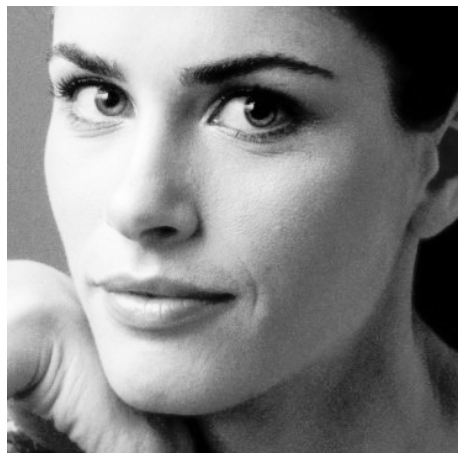
\includegraphics[width=\textwidth]{resources/Annotation_Correction/Fig_Intro/intro_0_0}
    \hfill
    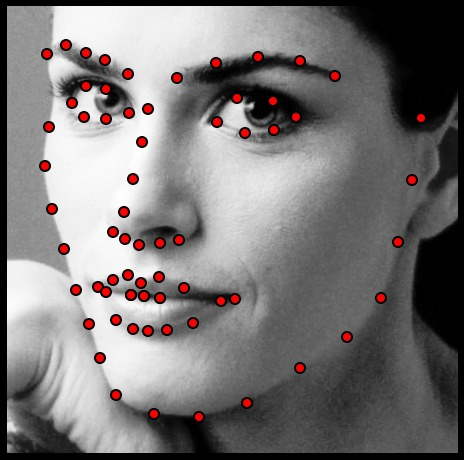
\includegraphics[width=\textwidth]{resources/Annotation_Correction/Fig_Intro/intro_0_1}
    \hfill
    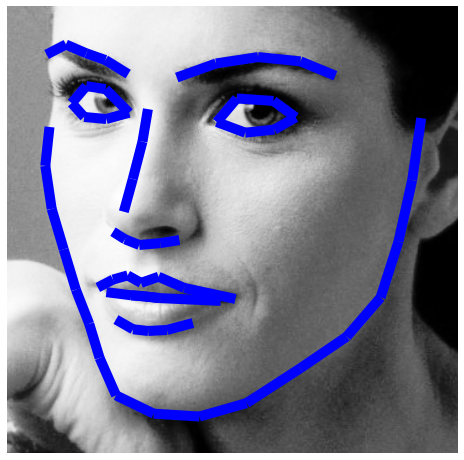
\includegraphics[width=\textwidth]{resources/Annotation_Correction/Fig_Intro/intro_0_2}
    \\
    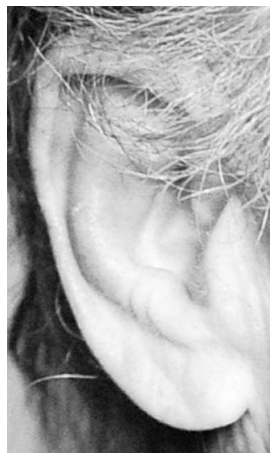
\includegraphics[width=\textwidth]{resources/Annotation_Correction/Fig_Intro/intro_1_0}
    \hfill
    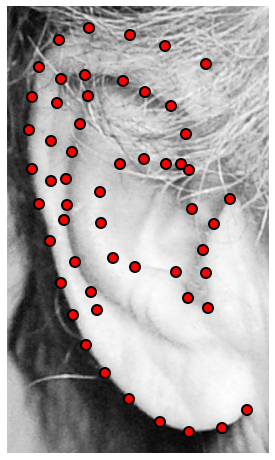
\includegraphics[width=\textwidth]{resources/Annotation_Correction/Fig_Intro/intro_1_1}
    \hfill
    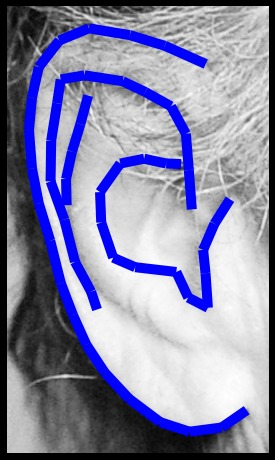
\includegraphics[width=\textwidth]{resources/Annotation_Correction/Fig_Intro/intro_1_2}
    \hfill
    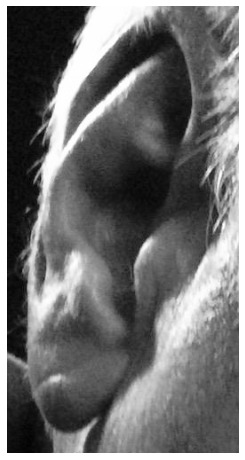
\includegraphics[width=\textwidth]{resources/Annotation_Correction/Fig_Intro/intro_1_3}
    \hfill
    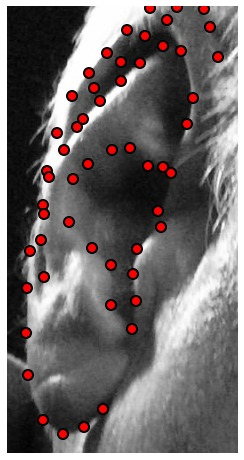
\includegraphics[width=\textwidth]{resources/Annotation_Correction/Fig_Intro/intro_1_4}
    \hfill
    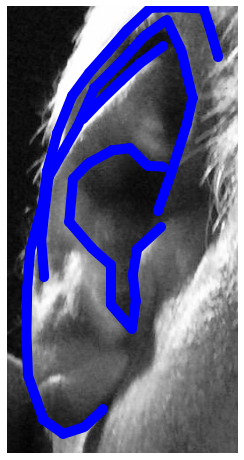
\includegraphics[width=\textwidth]{resources/Annotation_Correction/Fig_Intro/intro_1_5}
    \\
    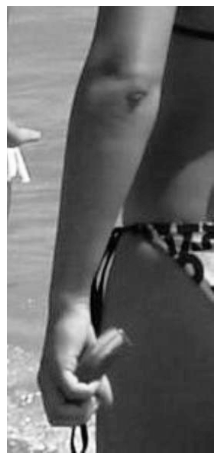
\includegraphics[width=\textwidth]{resources/Annotation_Correction/Fig_Intro/intro_2_0}
    \hfill
    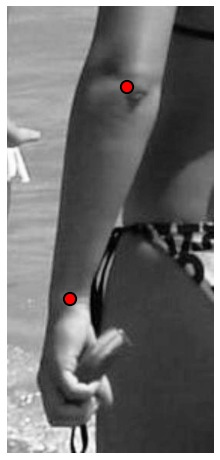
\includegraphics[width=\textwidth]{resources/Annotation_Correction/Fig_Intro/intro_2_1}
    \hfill
    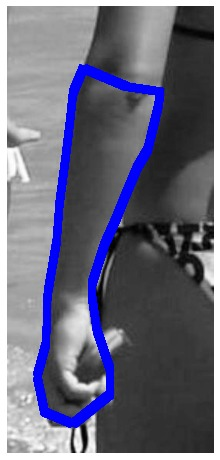
\includegraphics[width=\textwidth]{resources/Annotation_Correction/Fig_Intro/intro_2_2}
    \hfill
    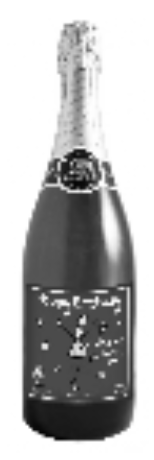
\includegraphics[width=\textwidth]{resources/Annotation_Correction/Fig_Intro/intro_2_3}
    \hfill
    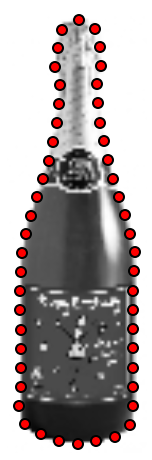
\includegraphics[width=\textwidth]{resources/Annotation_Correction/Fig_Intro/intro_2_4}
    \hfill
    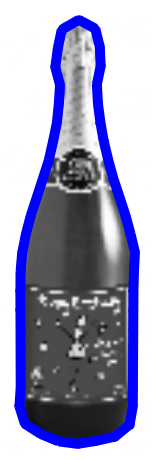
\includegraphics[width=\textwidth]{resources/Annotation_Correction/Fig_Intro/intro_2_5}
    \\
    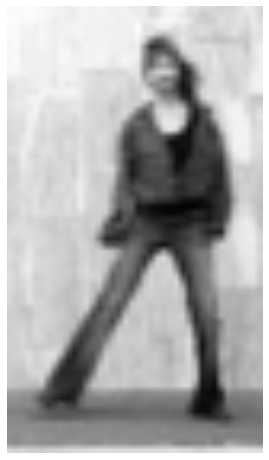
\includegraphics[width=\textwidth]{resources/Annotation_Correction/Fig_Intro/intro_3_0}
    \hfill
    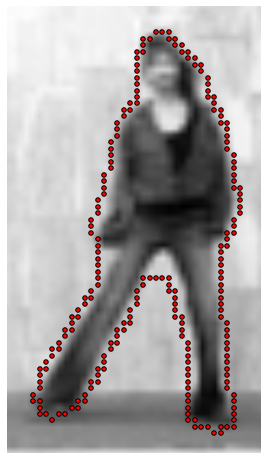
\includegraphics[width=\textwidth]{resources/Annotation_Correction/Fig_Intro/intro_3_1}
    \hfill
    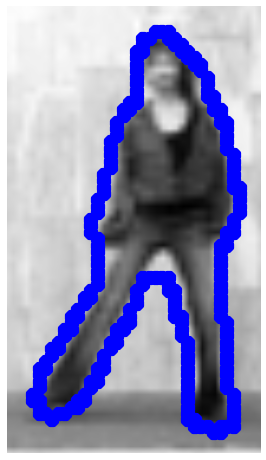
\includegraphics[width=\textwidth]{resources/Annotation_Correction/Fig_Intro/intro_3_2}
    \hfill
    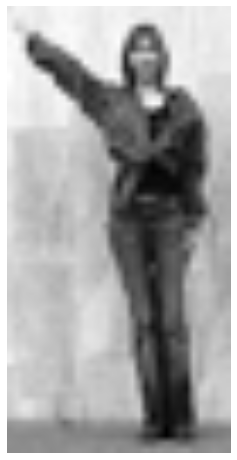
\includegraphics[width=\textwidth]{resources/Annotation_Correction/Fig_Intro/intro_3_3}
    \hfill
    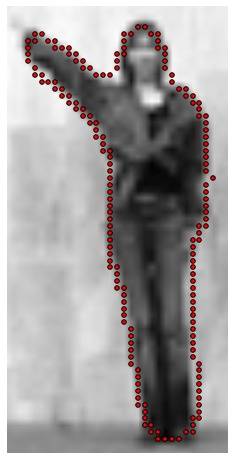
\includegraphics[width=\textwidth]{resources/Annotation_Correction/Fig_Intro/intro_3_4}
    \hfill
    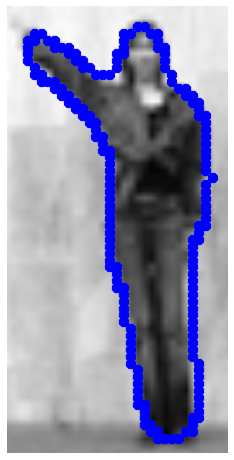
\includegraphics[width=\textwidth]{resources/Annotation_Correction/Fig_Intro/intro_3_5}
    \caption{Demonstration of classical landmark annotation and curve annotation of faces, ears, bottles and human actions.}
    \label{fig:intro}
\end{figure}

Building and fitting statistical deformable models (SDMs) of objects is a well-studied and popular area in the intersection of computer vision and machine learning~\cite{Cootes1995, Cootes2001, Matthews2004, Saragih2011, Belhumeur2011, Zhu2012, Xiong2013}, where SDMs have been widely applied on object detection, part localisation, model reconstruction, fitting, recognition and tracking using manual annotated data. In recent past, We have witnessed tremendous developments in building and fitting models of human face and body using images captured in unconstrained recording conditions, usually referred to as "in-the-wild"~\cite{Belhumeur2011, Cao2012, Zhu2012, Xiong2013, Asthana2013, Tzimiropoulos2014, Asthana2014}. This is attributed to: 
\begin{itemize}

\item The abundance of complex visual data, spread mostly through the internet via web services such as Youtube, Flickr and Google Images. The latter has led to the development of large databases of "in-the-wild" images of human faces and bodies~\cite{Belhumeur2011, Le2012, Zhu2012, Burgos2013}. Equally important is the task of manual annotation of images with regards to face and body parts and that has been undertaken by several research teams~\cite{sagonas_iccv_300w_2013}.

\item The development of powerful visual features, able to describe objects and its parts in a robust manner (e.g., Scale Invariant Feature Transforms (SIFT)~\cite{lowe1999object}, Histogram of Oriented Gradients (HoGs)~\cite{Dalal2005} and recently Deep Convolutional Neural Networks~\cite{sermanet2013overfeat}), as well as generative and discriminative methodologies for learning deformable models. 

\end{itemize}

Nevertheless, there are two drawbacks on building deformable models that rely on landmarks: 
\begin{itemize}

\item Annotating with regards to consistent landmark annotation is extremely time consuming, tedious and labour intensive work~\cite{sagonas_iccv_300w_2013}, which usually can be performed by a trained person. Furthermore, for many objects it requires a highly skilled person to identify and annotate a set of images with regards to a consistent set of landmarks. For example human ears have very complicated inner structures (e.g. helix, crus antihelicis, scapha, tragus, lobe etc.) which differs remarkably between ears. Moreover, certain ear parts, such as  Fossa Triangularies and Crus Helicis, do not appear in all ears and  their visibility is highly sensitive to pose and illumination variation. Figure \ref{fig:formal_ear} demonstrated major feature components of a standard ear~\cite{Pflug2012}. 

\begin{figure}[ht]
    \centering
    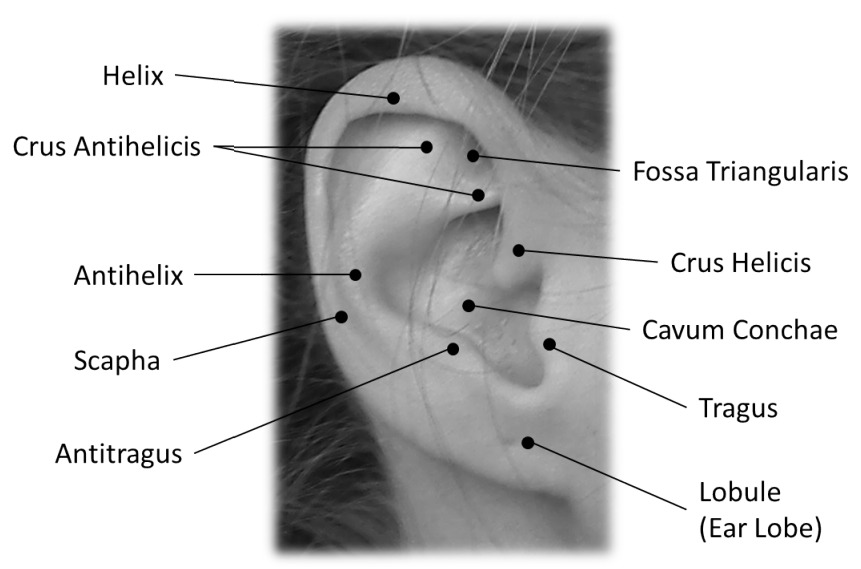
\includegraphics[width=0.5\textwidth]{resources/Background/formal_ear} 
    \caption{Ear with Clear Features}
    \label{fig:formal_ear}
\end{figure}

\begin{figure}[ht]
    \centering
    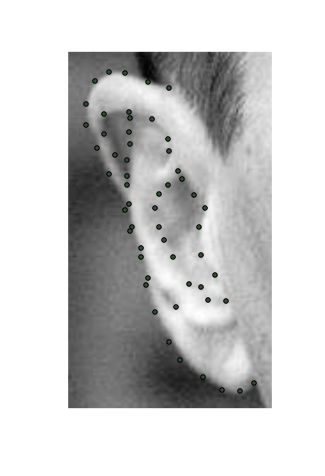
\includegraphics[width=0.22\textwidth]{resources/Background/hidden_feature_ear} 
    \hfill
    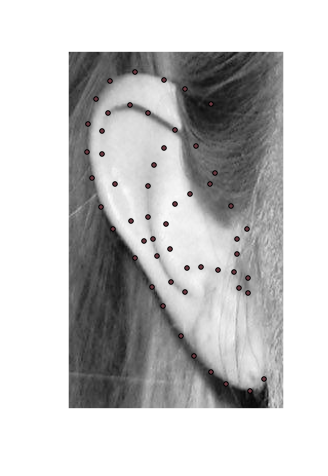
\includegraphics[width=0.22\textwidth]{resources/Background/hidden_feature_ear2} 
    \hfill
    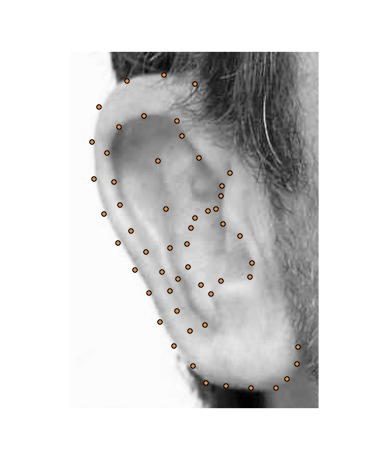
\includegraphics[width=0.22\textwidth]{resources/Background/hidden_feature_ear3} 
    \hfill
    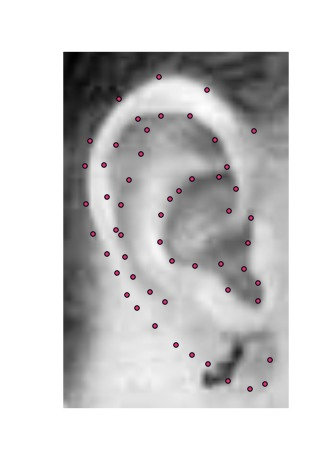
\includegraphics[width=0.22\textwidth]{resources/Background/hidden_feature_ear4} 
    \caption{Ears with Partial Features}
    \label{fig:hfe}
\end{figure}

But from Figure \ref{fig:hfe}, none of the shown ears has all features displayed clearly comparing to features of the standard ear. Some features are missing due to the pose variation or illumination (e.g. Figure \ref{fig:hfe1} has antihelix overlapped with helix) while some are because of the nature of ear, not all features exist on every ears (e.g. Figure \ref{fig:hfe2} has unclear crus antihelics, fossa triangularis and crus helicis are missing). The caption of each image in Figure \ref{fig:hfe} states the differences comparing to the standard ear.

\item The nature of many deformable objects does not allow them to be consistently annotated with regards to a set of landmarks (e.g. bottles, fruits etc.). Also the boundary/outline of objects, such as faces, ears, body can be very difficultly annotated consistently, Figure \ref{fig:intro}. That is why many state-of-the-art methods opt to leave the boundary out for comparison~\cite{Tzimiropoulos2014, Asthana2014}. The majority of the state-of-the-art methods for landmark-based deformable models~\cite{Cao2012, Zhu2012, Xiong2013, Tzimiropoulos2014, Asthana2014} are not applicable for objects with no consistent set of landmarks. 

\end{itemize}

To illustrate how time consuming careful annotation of ears is we lay down our own experience. A trained annotator needs an average of 4 minutes per image for the manual annotation of 55 landmarks. This means that the annotation of 1000 images requires a total of about 67 hours. 
Furthermore, training and fatigue largely influence the annotation accuracy. Hence, a second pass on the annotated data is, in many cases, necessary. Due to the fact that manual annotation is a rather costly and labour-intensive procedure, unsupervised learning of deformable models for the tasks of alignment has recently attracted some attention~\cite{kokkinos2007unsupervised,jojic2006escaping,jiang2009learning,liu2009simultaneous,baker2004automatic,cox2008least,cootes2004groupwise,frey2003learning}. Nevertheless, the method of~\cite{antonakos2014automatic} requires a consistent set of shapes annotated with landmarks to perform deformable face congealing. Finally, since the problem of fully unsupervised discovery of the deformations of arbitrary objects is a very difficult and ill-posed problems the limited number of methods that have been applied for the task cannot be applied for arbitrary collection of images collected "in-the-wild". 

% TODO: Diffeomorphic Registration
Researches~\cite{cootes2004groupwise,cootes2004diffeomorphic,cootes2010computing,rueckert2006diffeomorphic,rueckert1999nonrigid,koelstra2010dynamic} also introduced methods for diffeomorphic image/shape registration, which put shapes in dense correspondence. Transformations between pairwise/groupwise images are diffeomorphic. Diffeomorphic deformations are smooth and invertible that, to be more specific, every points in shape $A$ have one-to-one correspondence with points in shape $B$, and vise versa. However, researches have shown there is no gaurentee that diffeomorphic algorithms can outperform algorithms with no diffeomorphism\cite{crum2004framework}.

We provide a solution for annotating an object with regards to its deformations that requires considerable less effort and in the same time can be used to define statistical deformations for objects without consistent set of landmarks. That is, we argue that it is better to annotate an object with regards to a set of continues lines that describe the shape of the object. An example is provided in Figure \ref{fig:intro} where the shape of the facial parts is annotated with continuous lines instead of a number of discrete landmarks. Similarly, the shape annotations for the ear, a bottle and human body is shown in Figure \ref{fig:intro} Annotating facial images by following this procedure takes less than 30 secs per image. Furthermore, these shapes can be automatically produced by recent methods that perform discriminative segmentation of objects. 

Furthermore, we show that flow methods have mature enough so that it can be used to densely annotate the proposed shapes using simple, as well as more recent and robust shape representations methods~\cite{Garg2013,Nguyen2013}.  In particular, to build dense correspondence between independent shapes, we apply optical flow on shapes with low rank constrains, so we name it shape flow. Optical flow is originally applied to video sequences that several assumptions holds, illumination consistency and motion smoothness, while shapes having no motion smoothness completely as all training data are independent. Low rank constrain plays important role to simulate motion smoothness assumption. 

We show that this way dense correspondences between images can be established and dense Active Appearance Models (AAMs) can be build on top of that. We show that the proposed methodology even though not tailored to landmark localization can be applied for landmark localization achieving very good performance. Finally, we demonstrate the performance of the proposed methodology for describing objects that do not have consistent landmarks. To the best of our knowledge this is the first methodology which can create a dense statistical model for AAM which can operate in "in-the-wild".

Summarizing, the contributions proposed in this report are:
\begin{itemize}
  \item Constructing SDMs using training data with inconsistent annotation.
  \item Introduce highly effective curve annotation which tremendously reduces manual work overload but maintains same performance level against state-of-the-art SDMs.
  \item Building dense correspondent SDMs with shape flow
\end{itemize}


\section{Publications}
A list of publications are provided in this section. All publications were authored during the course of this Ph.D. thesis. There are two sections of publications: 1) publications that are directly related to the contents of this thesis (Section~\ref{label:related_pubs}) and 2) publications that are relatively relevant (Section~\ref{label:other_pubs}).

\subsection{Related Publications}
\label{label:related_pubs}

\begin{itemize}
  \item Ear Journal (TODO: To be complete)
  \item IJCV DenseReg and Pose Journal
  \item FG2018 Dense Pose
  \item FG2017 Ear Deformable Models
  \item CVPR2016: Annotation Correction
\end{itemize}

\subsection{Other Publications}
\label{label:other_pubs}

\begin{itemize}
  \item DeepMind & Brain Project: publication somewhere (could be NIPS)
  \item UVGAN
  \item Joint Multi-view Face Alignment in the Wild
  \item Marginal Loss for Deep Face Recognition
  \item Semi-autonomous Data Enrichment Based on Cross-task Labelling of Missing Targets for Holistic Speech Analysis
\end{itemize}

\subsection{Outline}



\chapter{Background Theory}
\label{ch:background}
\minitoc

This section briefly introduce fundamental technologies that current research based on. Section \ref{sec:bg_aam} explains the manner of constructing statistical deformable models using active appearance model. Section \ref{sec:bg_icp} briefly described the mechanical of Iterative Closest Points and the reason of using ICP for pre-processing. Section \ref{sec:bg_svs} introduces a shape discriminator which is infinitely differentiable. Section \ref{sec:bg_opticalflow} brings the technologies of registering video sequences. Our research takes the idea from optical flow in order to put shapes in dense correspondence. Section \ref{sec:SSD} presents the algorithm of steepest descend for minimising error function when fitting objects.

\section{Active Appearance Model (AAM)}
\label{sec:bg_aam}
An Active Appearance Model (AAM) is a combination of linear statistical shape and appearance model with corresponding fitting algorithms \cite{Matthews2004, Cootes2001}. AAM separate that model in two parts, shape model and appearance model. 

\subsection{Shape Model}
Shapes are defined as vertexes of a mesh. A shape model is a function that can express arbitrary shapes by using a base shape plus a linear combination of shape vectors. Mathematical definition of shape model shown below:
\begin{equation}
s=s_0+\sum^n_{i=1}p_i s_i
\end{equation}
where shape $s$ is expressed by base shape $s_0$ plus linear combination of shape vectors $s_i$, each having coefficient $p_i$. Note that $s_i$ need to be orthonormal. In general, shape model are generated by applying Principle Component Analysis (PCA). Therefore $s_0$ is the mean shape with $s_i$ are eigenvectors(principle components).

\subsection{Appearance Model}
\label{sec:appearance_model}
Appearances are defined as pixels lie inside base shape $s0$. Similar to shape models, appearance models are defined in same format, a base appearance plus linear combination of appearance vectors. Mathematical definition of appearance model is expressed below:
\begin{equation}
A(x)=A_0(x)+\sum^m_{i=1}\lambda_iA_i(x)
\end{equation}
where $x \in s0$, appearance $A(x)$ is expressed by base appearance $A_0(x)$ plus linear combination of appearance vectors $A_i(x)$, each having coefficient $\lambda_i$. Note that $A_i(x)$ need to be orthonormal. In general, appearance model are generated by applying Principle Component Analysis (PCA). Therefore $A_0(x)$ is the mean appearance with $A_i(x)$ are eigenvectors(principle components).

\subsection{AAM Instance}
Active Appearance Model combines shape model and appearance model to generate instances. Instance generating procedure is starting with compute warping from base shape $s_0$ to instance shape $s$, to be more specific, piecewise affine warp in general. The warp is required to map appearance instance $A(x)$ to shape instance $s$ since appearance instance is built on base shape $s_0$. The way piecewise affine works is finding corresponding triangles in both base shape and instance shape, then for each pixels within a triangle on $s_0$, finding position of the pixel of same triangle in $s$. The final model instance should satisfies  following expression:
\begin{equation}
M(W(x;p))=A(x)
\end{equation}
where $M$ is AAM instance and $W(x;p)$ represent piecewise affine warp.

\subsection{AAM Fitting}
In the case of fitting an AAM to an input image $I(x)$, aam instance $M(W(x;p))=A(x)$ should be similar as $I(x)$. For any pixel $x$ in base shape $s_0$, the corresponding pixel in the input image is $W(x;p)$. Appearance of pixel $x$ are defined as $A(x)=A_0(x)+\sum^m_{i=1}\lambda_iA_i(x)$ mentioned in section \ref{sec:appearance_model}. For pixel $W(x;p)$, appearance of input image is expressed as $I(W(x;p))$. A formal fitting algorithm can now be defined: the objective is to discover optimal AAM instance that fit given input image maximumly. In other words, we want to minimise following error function to minimise difference between $A(x)$ and $I(W(x;p))$:
\begin{equation} 
\label{eq:aamfittingbase}
E(x)=||A_0(x)+\sum^m_{i=1}\lambda_iA_i(x)-I(W(x;p))||^2
\end{equation}
where input image is denoted as $I$ and $||.||^2$ is the L2 norms. To be more specific, image $I$ is warped back onto base shape $s_0$ before computing difference against AAM instance appearance.

\subsection{Alternating Minimisation}
As the expression revealed, there are two variables contained ($p$ and $\lambda$) so it is of importance to minimise them simultaneously. As there is no dependency between AAM shape and appearance, solving $p$ and $\lambda$ alternatively is plausible. Considering creating a linear subspace, which is spanned by collection of appearance component vector $A_i$, denoted as $span(A_i)$ and $span(A_i)^\perp$ as orthogonal complement subspace. Therefore \ref{eq:aamfittingbase} can be rewrite as:
\begin{equation} 
\label{eq:aamfittingappearancevariance}
E(x)=||A_0(x)+\sum^m_{i=1}\lambda_iA_i(x)-I(W(x;p))||^2_{span(A_i)^\perp}+||A_0(x)+\sum^m_{i=1}\lambda_iA_i(x)-I(W(x;p))||^2_{span(A_i)}
\end{equation}
where $||.||^2_L$ is L2 norm of vector projected into linear subspace $L$. Because norm considers only orthogonal components of subspace $L$ so any components lies in $L$ can be dropped. So the above function can be optimised as:
\begin{equation} 
\label{eq:aamfittingappearancevariancesubspace}
E(x)=||A_0(x)-I(W(x;p))||^2_{span(A_i)^\perp}+||A_0(x)+\sum^m_{i=1}\lambda_iA_i(x)-I(W(x;p))||^2_{span(A_i)}
\end{equation}
The first section contains only variable $p$, therefore the optimal value of the equation can be found by first minimising $||A_0(x)-I(W(x;p))||^2_{span(A_i)^\perp}$ with respect to $p$ alone before substitute minimal $p$ value in $||A_0(x)+\sum^m_{i=1}\lambda_iA_i(x)-I(W(x;p))||^2_{span(A_i)}$ then minimise with respect to $\lambda$. Mathematical equations shown below:
\begin{equation}
\label{eq:minimisep}
\operatorname*{arg\,min}_p=||A_0(x)-I(W(x;p))||^2_{span(A_i)^\perp}
\end{equation}
Based on the assumption of basis vector $A_i$ are orthonormal, $\lambda$ can be computed with closed-form solution:
\begin{equation}
\label{eq:minimiselambda}
\lambda_i=\sum_{x\in s_0}A_i(x).[I(W(x;p))-A_0(x)]
\end{equation}

\subsection{Image Alignment}
Minimising equation \ref{eq:minimisep} also referenced as Image Alignment. The purpose of image alignment is finding constant template image in given input image \cite{Matthews2004}. 

\subsubsection{Lucas-Kanada Algorithm}
Using gradient descent method for image alignment was first introduced by Lucas Kanada by minimising square error between two images which having same form as equation \ref{eq:minimisep}. Solving $p$ is a nonlinear process as pixel value of an image generally unrelated to pixel coordinate. Lucas Kanada make the problem linear by solving the problem with an incremental parameter $\delta p$ with assumption that initial value of $p$ is known. Thus the problem can be solved iteratively for $\delta p$. Equation \ref{eq:minimisep} can now be solved with respect to $\delta p$ as:
\begin{equation}
\label{eq:minimisedp}
||A_0(x)-I(W(x;p+\delta p))||^2
\end{equation}
where $p$ gets updated at every iteration by $p=p+\delta p$. A Taylor expansion on above function gives:
\begin{equation}
\label{eq:minimisedptaylor}
||A_0(x)-I(W(x;p))-\nabla I\frac{\partial W}{\partial p} \delta p))||^2
\end{equation}
where $\frac{\partial W}{\partial p}$ is the Jacobian and $\nabla I$ is image gradient. $\delta p$ can be solved in closed form:
\begin{equation}
\label{eq:dp}
\delta p=\bm{H}^{-1}\sum_x[\nabla I\frac{\partial W}{\partial p}]^T[A_0(x)-I(W(x;p))]
\end{equation}
where $\bm{H}$ is the Hessian matrix:
\begin{equation}
\label{eq:hessian}
\bm{H}=\sum_x[\nabla I\frac{\partial W}{\partial p}]^T[\nabla I\frac{\partial W}{\partial p}]
\end{equation}
The new variable $p$ can now be updated by $p=p+\delta p$ before involving in next iteration of optimisation. Iterations ends when converged or specific criteria reached. 

However, Lucas-Kanada Gaussian-Newton descent is slow due to computational intensity on Hessian Matrix $\bm{H}$, which contains image gradient $\nabla I$ and warp Jacobian $\frac{\partial W}{\partial p}$ and both depends on $p$ but $p$ is varying at every iteration. Besides, computation of $\nabla I$ $\frac{\partial W}{\partial p}$ also slow.

\subsubsection{Forwards Compositional Algorithm}
\label{sec:fca}
Instead of updating $p$ from estimated $\delta p$ iteratively, \cite{Matthews2004} mentioned compositional algorithms of updating warp transformation. The cost function are:
\begin{equation}
\label{eq:forwardcomposition}
||A_0(x)-I(W(W(x;\delta p);p))||^2
\end{equation}
where $W(x;\delta p)$ denotes incremental warp. The update step of new warp $W(x;p)$ is:
\begin{equation}
W(x;p) = W(x;p)\circ W(x;\delta p)
\end{equation}
Applying Taylor expansion on equation \ref{eq:forwardcomposition} gives:
\begin{equation}
\label{eq:forwardcompositiontaylor}
||A_0(x)-I(W(W(x;0);p))-\nabla I(W(x;p))\frac{\partial W}{\partial p}\delta p||^2
\end{equation}
where $W(x;0)$ is the identical warp that $W(x;0) = x$. Comparing with equation \ref{eq:minimisedptaylor}, image gradient is now computed for $I(W(x;p))$. The key improvement is that update of warp is evaluation with respect to $p=0$ therefore Jacobian is now computed at $(x;0)$. Thus a constant Jacobian through all iterations so can be precomputed.

\subsubsection{Inverse Compositional Algorithm}
Inverse Compositional Algorithm are based on Forwards Compositional Algorithm that the purpose of template image $A_0(x)$ and input image $I$ are inversed to further improve performance by precomputing $\delta p$ and Hessian matrix \cite{Matthews2004}. Cost function for inverse compositional algorithm are:
\begin{equation}
\label{eq:inversecomposition}
||I(W(x;p))-A_0(W(x;\delta p))||^2
\end{equation}
where $W(x;\delta p)$ denotes incremental warp on template image. So the update step of new warp $W(x;p)$ is:
\begin{equation}
W(x;p) = W(x;p)\circ W(x;\delta p)^{-1}
\end{equation}
Applying Taylor expansion on equation \ref{eq:inversecomposition} gives:
\begin{equation}
\label{eq:inversecompositiontaylor}
||I(W(x;p))-A_0(W(x;\delta p))-\nabla A_0\frac{\partial W}{\partial p}\delta p||^2
\end{equation}
where $W(x;0)$ is the identical warp that $W(x;0) = x$. The closed form solution of $\delta p$ is:
\begin{equation}
\label{eq:dpic}
\delta p=\bm{H}^{-1}\sum_x[\nabla A_0\frac{\partial W}{\partial p}]^T[I(W(x;p))-A_0(x)]
\end{equation}
where $\bm{H}$ is the Hessian matrix:
\begin{equation}
\label{eq:hessianic}
\bm{H}=\sum_x[\nabla A_0\frac{\partial W}{\partial p}]^T[\nabla A_0\frac{\partial W}{\partial p}]
\end{equation}
As the equation states, image template $A_0$ is constant and $\frac{\partial W}{\partial p}$ is evaluated at $p=0$ same as the Jacobian part in forward compositional algorithm. Therefore both $\delta p$ and Hessian $\bm{H}$ can be precomputed before optimising cost function. 

\subsection{Pseudo Algorithms}

The pseudo code of AAM fitting using inverse compositional algorithm is shown in Algorithm \ref{alg:aam}\cite{Matthews2004}:

\begin{algorithm}[ht]
\caption{Fitting Active Appearance Model with Inverse Compositional Algorithm}
\label{alg:aam}
Compute gradient $\nabla A_0$ of image template $A_0(x)$\;
Compute Jacobian $\frac{\partial W}{\partial p}$ at $(x;0)$\;
Compute Hessian matrix $H$\;
\While{not converged or criteria not met}{
    Warp input image $I$ with transform $W(x;p)$\;
    Compute error image $I(W(x;p))-A_0(x)$\;
    Compute $\delta p$ by multiplying inverse Hessian matrix $H^{-1}$\;
    Update warp by $W(x;p) = W(x;p)\circ W(x;\delta p)^{-1}$\;
    Update $\lambda$ by $\lambda_i=\sum_{x\in s_0}A_i(x).[I(W(x;p))-A_0(x)]$\;
}  
\end{algorithm}


% AAM is trained using a set of images where each image contains clear annotated images using same number of landmarks. Shape model is trained using landmark coordinates before applying PCA on shapes to produce a mean shape with some eigenvectors to control the deformation of mean shape. For training appearance model, training images are warped to a reference frame, which contains landmarks of mean shape, so we have different objects with same shape but different texture. Then PCA is used again applying on the warped images to generate mean appearance with eigenvectors controlling variations of texture. Fitting an AAM model to a new image is using Lucas Kanade Alternating Inverse Composition algorithm which is clearly explained in references \cite{Matthews}.
\section{ICP \& NICP}
\label{sec:bg_icp}
\subsection{Iterative Closest Point}
Iterative Closest Point (ICP) is an algorithm for aligning two different point clouds\cite{Besl1992}. In the situation of aligning point cloud A to point cloud B (named source and target correspondingly), the algorithm finds the transformation matrix that best matches source to target. The procedure can be briefly summarised as following steps:
\begin{itemize}
  \item For each point in source, finding corresponding closest point in target.
  \item Calculating optimal rotation, translation and scaling transform to minimise difference (measured in point-to-point mean square error) between source and points generated in previous step.
  \item Transform source using translation calculated in previous step to obtain new source.
  \item Iterate until converge or special criteria satisfied.
\end{itemize}
\cite{Besl1992} shows ICP convergence can be proved that it will always converge to a local minimum.

\subsection{Non-rigid Iterative Closest Point}
Although ICP provided notable solution of aligning point clouds, it provides only rigid alignment that finding the best affine transform between source and target. For objects e.g. faces, ears, human poses, bottles and objects that are highly deformable, ICP is weak at model local changes and produces biased result due to non-rigid deformation.

Non-rigid Iterative Closest Point (NICP) are an extension of ICP having enabling source to deform to fit target without breaking the property of guaranteed convergence\cite{Amberg2007}. A new term stiffness is introduced in order to constrain the degree of deformation. The fundamental idea is to incrementally apply ICP with stiffness where stiffness are scaling from high to low value at each iteration. To be specific, at initial iteration, the algorithm turned to apply rigid ICP on source, but source are allowed to deform in later iteration with increasingly extent. After converging, each point of source have one-to-one correspondence of points on target.

In the situation of registering source $S$ to template $T$, $S$ are defined as mesh $(V,E)$ where $V$ are vertices and $E$ are edges with corresponding amount $n, m$. Template $T$ can have vertices only without defining edges. Registering $S$ to $T$ means computing a transformation matrix $X$ so that $V(X)$ is the projection of each points on target. Proper definition of $X$ are:
\begin{equation}
\label{eq:nicpX}
X=[X_1,X_2,\dotsc,X_n]^T
\end{equation}
where $X_i$ is affine $3\times 4$ transformation matrix so $X$ are $4n\time 3$ matrix. The comprehensive cost function of optimising $X$ are:
\begin{equation}
E(X)=E_d(X)+\alpha E_s(X)+\beta E_l(X)
\end{equation}
where $E_d(X)$ is distance penalty term, $E_s(X)$ is stiffness penalty term and $E_l(X)$ is landmark penalty term. Definitions of each term are detailedly introduced in following sections \ref{sec:nicpdt}, \ref{sec:nicpst} and \ref{sec:nicplt}.

\subsubsection{Distance Penalty Term}
\label{sec:nicpdt}

Distance between $S$ and $T$ are defined using Euclidean Distance. The distance penalty term and corresponding matrix form is defined as~\cite{Amberg2007}:

\begin{align}
\label{eq:nicpdt}
E_d(X) &= \sum_{i=1}^n{w_i || X_i v_i - u_i ||^2} 
\\ &=
\begin{Vmatrix}
    (W \otimes I_3) 
    \begin{pmatrix}
        \begin{bmatrix}
        X_1 &  &  \\  & \ddots &  \\ &  & X_n
        \end{bmatrix}
        \begin{bmatrix}
        v_1 \\ \vdots \\ v_n
        \end{bmatrix}
        -
        \begin{bmatrix}
        u_1 \\ \vdots \\ u_n
        \end{bmatrix}
    \end{pmatrix}
\end{Vmatrix}
^2
\end{align}

where $v_i \in V$ are assumed having format $[x,y,z,1]^T$, $u_i \in T$ is corresponding closest point with same format of $v_i$, Euclidean distance between $v_i$ and $u_i$ is weighted by $w_i$. For matrix form, $W$ has form $\text{trace}(w_1,...,w_n)$ and performs Kronecker tensor product with an identity matrix of shape $3 \times 3$. 

By defining $D = \text{trace}(v_1,\dotsc,v_n)$ and $U=[u_1,\dotsc,u_n]^T$, above equation can be further simplified as:
\begin{equation}
E_d(X) = ||W(DX-U)||^2_F
\end{equation}

\subsubsection{Stiffness Penalty Term}
\label{sec:nicpst}

Stiffness term is introduced to have constrain on deformation. In other word, stiffness maintains the neighbouring  correlation for each vertex. A significant deformation of one vertex can cause remarkable penalty on neighbouring vertices. Therefore source mesh cannot deform completely freely but with regularisation. The matrix form of stiffness penalty cost function defined as~\cite{Amberg2007}:
\begin{equation}
E_s(X)=||(M \otimes G)X||^2_F
\end{equation}
where $M$ expresses the connectivity of vertices with $m \times n$ that each row $r$ represent an edge, for edge connecting vertices $(i,j)$, $M_{ri}=-1$ and $M_{rj}=1$. $G=\text{trace}(1,1,1,\gamma)$, where $\gamma$ used to weight skew and rotation part of deformation.

\subsubsection{Landmark Penalty Term}
\label{sec:nicplt}

Landmark penalty term functioning similar as distance term. It can be assumed as a sparse version of distance term with exact landmark correspondence instead of looking up for closest points. Formal definition are~\cite{Amberg2007}:
\begin{equation}
E_l(X)=||D_LX-U_L||^2_F
\end{equation}
where $D_L$ are rows from matrix $D$ that related to landmark points and similarly $U_L$ are of format $[l_1,\dotsc,l_l]^T$ with $l_i$ as landmark points.

\cite{Amberg2007} shown landmarks term is optional. Although landmark term accelerated converge rate, NICP still produced desirable result without this term.

\subsubsection{Comprehensive Cost Function}
As each of penalty terms are defined in details above, the finalised cost function can be expressed:
\begin{align}
\label{eq:nicpfinal}
E(X) &= 
\begin{Vmatrix}
    \begin{bmatrix}
        \alpha M \otimes G \\ WD \\ \beta D_L
    \end{bmatrix}
    X- 
    \begin{bmatrix}
        0 \\ WU \\ U_L
    \end{bmatrix}
\end{Vmatrix}
^2_F \\
&= ||AX-B||^2_F,
\end{align}
where $X$ can be solved directly by setting the derivative of $E(X)$ to zero. So $X$ has a closed-form solution:
\begin{equation}
\label{eq:nicpx}
X=(A^TA)^{-1}A^TB
\end{equation}
which simply is the product of pseudo-inverse of matrix $A$ and matrix $B$. Therefore in each step, the deformation can be found directly for fixed $\alpha$ and $\beta$. Since landmark term is optional, the final algorithm considers only varying stiffness weighting. Pseudo code are shown below~\cite{Amberg2007}:
\begin{algorithm}[ht]
\caption{Non-rigid Iterative Closest Point Algorithm}
\label{alg:nicp}
Initialise $X^0$ as identical transformation\;
\For{$\alpha \in [\alpha^1,\dotsc,\alpha^p] \& \alpha_i > \alpha_{i+1}$}{
    \While{$||X^j-X^{j-1}||^2_F > \varepsilon$}{
        Calculate new source $S=(V(X^{j-1}),E)$\;
        Find optimal $X^j$ between $S$ and $T$ using equation \ref{eq:nicpx}\;
    }
}
Return $X$\;
\end{algorithm}

As Nonrigid ICP declared that it preserved convergence feature from ICP so the algorithm \ref{alg:nicp} also gauranteed termination. Detailed discussion convergence preservation can be found in~\cite{Amberg2007}.
\section{Support Vector Shape (SVS)}
\label{sec:bg_svs}
Support Vector Shape (SVS) introduces an implicit 2D or 3D shape discrimination based on Support Vector Machine (SVM) \cite{Nguyen2013}. Shapes are defined as decision function from training SVM with Radial Basis Function (RBF) kernel. SVS representation introduces several powerful advantages:
\begin{itemize}
  \item Expressing shapes against noise, fragmentation and artifacts.
  \item Presenting shapes with invariance of scale, rotation and translation.
  \item Producing shapes features reliably.
\end{itemize}

\subsection{Training Decision Function}
SVS shape descriptor involves SVM to learn decision function that will be able to distinguish points from whether they lies in given shape with a probability. To represent shapes with continuous function, SVM with RBF kernel gives an analytical solution. RBF kernel function can map data with arbitrary features to an infinite-dimension space where given shape can be linear separated from other points. The decision function of SVS is defined as \cite{Nguyen2013}:
\begin{equation}
\label{eq:svsdf}
f(x)=\sum^m_{i=1}\alpha_i[\Phi(x).\Phi(x^*_i)]
\end{equation}
where $x^*_i$ are support vectors with corresponding weight $\alpha_i$ and $\Phi$ is a mapping function in product space $H$ where the RBF kernel function replaces the dot product as:
\begin{equation}
\label{eq:svskernel}
k(x,x^*_i)=\Phi(x).\Phi(x^*_i)=exp(-\gamma||x-x^*_i||^2)
\end{equation}
Combining equation \ref{eq:svsdf} and \ref{eq:svskernel} gives a comprehensive expression:
\begin{equation}
\label{eq:svs}
f(x)=\sum^m_{i=1}\alpha_iexp(-\gamma||x-x^*_i||^2)
\end{equation}

For training SVS, arbitrary points lies in shapes are chosen as positive training samples, while random external points that close to shape contour are sampled as negative training set. Lastly, v-SVM \cite{scholkopf2001estimating} are employed to learn the decision function to separate positive and negative points.

\begin{figure}
    \centering
    \begin{subfigure}[b]{0.5\linewidth}
        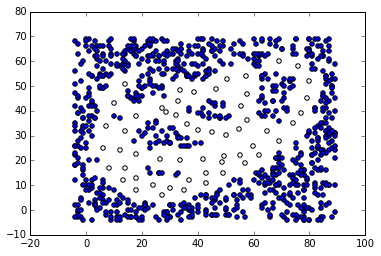
\includegraphics[width=\textwidth]{resources/Background/svs_samples} 
        \caption{Sampled Positive(white) and Negative(blue) Points}
        \label{fig:svs1}
    \end{subfigure}
    \hfill
    \begin{subfigure}[b]{0.4\linewidth}
        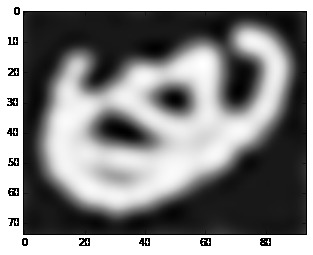
\includegraphics[width=\textwidth]{resources/Background/trained_svs} 
        \caption{Trained SVS Shape}
        \label{fig:svs2}
    \end{subfigure}
    \caption{SVS Training Points and Trained Shape}
\end{figure}

Figure \ref{fig:svs1} shows the training points where blue and white are marked as negative and positive respectively. Figure \ref{fig:svs2} revealed the final trained SVS plot, in which write colour means points are considered as part of shape with high possibility while black colour means the opposite.

\subsection{SVS Feature Points}
With SVS shape representation, reliable scale, rotation and translation invariant feature points can be retrieved based on decision function \ref{eq:svs}. Four types of feature points are produced by SVS representation: gradient based, support vector based, curvature based and entropy based feature points.

\subsubsection{Gradient Based Feature}
The gradient feature is reliable because gradient orientation is stable while gradient magnitude differs by constant factors. Gradient can be found by finding first derivative of $f(x)$ \cite{Nguyen2013}:
\begin{equation}
\label{eq:svsgrad}
\nabla f(x)=2\gamma\sum^m_{i=1}\alpha_iexp(-\gamma||x-x^*_i||^2)(x^*_i-x)
\end{equation}
where gradient orientation given by $\frac{\nabla f(X)}{||\nabla f(X)||}$. Experiments in \cite{Nguyen2013} shows gradient is stable for higher gradient magnitude points.

\subsubsection{Support Vector Based Feature}
Support vectors are claimed suitable to be feature points on it selves, due to their discriminative power of training decision function and gradient. But support vectors are sensitive to object shape. Shape deformation affects support vectors significantly.

\subsubsection{Curvature Based Feature}
Curvature based features tend to calculate points with sharp curves on decision function. Especially for 2D situation, eigenvalues of Hessian matrix is close related to curvature value:
\begin{equation}
\label{eq:svshessian}
H=
\begin{bmatrix}
    \frac{\partial^2f}{\partial x^2_1} & \frac{\partial^2f}{\partial x_1\partial x_2}\\
    \frac{\partial^2f}{\partial x_1\partial x_2} & \frac{\partial^2f}{\partial x^2_2}
\end{bmatrix}
=Q
\begin{bmatrix}
    \lambda_1 & 0\\
    0 & \lambda_2
\end{bmatrix}
Q^{-1}
\end{equation}
where points $(x_1,x_2)$ having large curvature associated with large eigenvalue in both dimension. Curvature features are highly discriminative but is not appropriate for shape matching.

\subsubsection{Entropy Based Feature}
Another similar measurement for selecting feature points is using entropy of local gradient orientation. The entropy is computed as \cite{Nguyen2013}:
\begin{equation}
\label{eq:svsentropy}
-\sum_{i=1}^np_i\log_2(p_i)
\end{equation}
where $p_i$ is the weight of bin $i$ and $n$ is number of bins in histogram. High entropy is proportional to gradient directional variation. The feature also provides highly reliable descriptor but are difficult to compute in higher dimension.
\section{Optical Flow}
\label{sec:bg_opticalflow}
Optical Flow is the motion of objects revealed in image sequences or videos \cite{fleet2006optical},\cite{Sun2010}. By estimating optical flow between frames in video sequences, motion, translation, deformation and many feature can be revealed. Optical flow is applicable under specific assumptions:
\begin{itemize}
  \item Motion of objects is smooth and gradually over time.
  \item Illumination is relatively consistent in given sequence. To be more specific, the pixel measurement in a small region remain the same despite of location changes.
\end{itemize}
A flow between two consecutive frames defines pixel movement from former frame to later frame. Defining former frame as \(I_n(i,j)\) where \(i,j\) represent pixel coordinate, the later frame is defined as \(I_{n+1}(i+u_{i,j},j+v_{i,j})\) where \(u_{i,j},v_{i,j}\) are horizontal and vertical translation of pixel (\(i,j\)). The fundamental algorithm of optimal optic flow is find a set of $u, v$ (flow directions) that minimised the objective error function:
\begin{equation}
E(p)=\sum^f_{n=1}\sum^{p}_{i,j\in p}[I_n(i,j)-I_{n+1}(i+u_{i,j},j+v_{i,j})]+regularisation
\end{equation}
where $f$ is number of frames in target sequence, $p$ is set of pixels in frame. Generally the error function contains a regularization term to prevent over fitting. Recent researches also suggest appending subspace constrains to error function \cite{Garg2013, Garg, Garg2013a}. 

\begin{figure}[h]
\centering
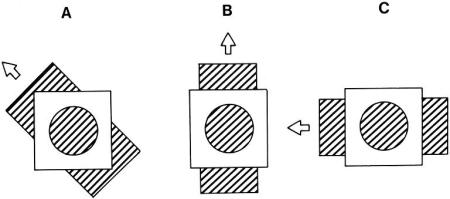
\includegraphics[width=0.9\textwidth]{resources/Background/aperture_problem}
\caption{Aperture Problem}
\label{fig:aperture_problem}
\end{figure}

\subsection{Aperture Problem}

Optical flow suffers from Aperture Problem. the aperture problem occur when determine global motion of objects from a small fraction of observation field. Figure \ref{fig:aperture_problem} demonstrate a situation when aperture problem occurs. Squares A, B and C all having different motion direction. But from only the circle observation field, objects are all classified as moving towards top left.

% Optical Flow is the motion of objects revealed in image sequences or videos \cite{fleet2006optical},\cite{Sun2010}. A flow between two consecutive frames is how pixels moves from former frame to later one. If we define former frame as \(I_1(i,j)\) where \(i,j\) represent pixel index, the later frame can defined as \(I_2(i+u_{i,j},j+v_{i,j})\) where \(u_{i,j},v_{i,j}\) are horizontal and vertical flow direction of pixel (\(i,j\)). An optimal optic flow is the set of $u, v$ (flow directions) that minimised the objective function \(\sum[I_1(i,j)-I_2(i+u_{i,j},j+v_{i,j})]\).

% In our situation, we use the idea of optical flow and apply on set of images so the flow direction should represent the correlation between objects in this case ears. Our Target is to build deformable models based on flows with an extension of deformation field where each deformed shapes are correlated. We build a flow between objects and try to minimising the following objective functions in terms of p and v.

% \begin{equation} ||I^t_p-I^{t-1}_p|| + ||U-Av||_f^2 + \sum[TV(Av)] + v.L.v^T\end{equation}

% Where \(p\) is an optimal parameter that miminise the difference between consecutive frames. \(U\) is the supervising data flow and A is eigenflow matrix with corresponding weight parameter v. The term \(\sum[TV(Av)]\) is the total variation and \(v.L.v(T)\) is used to smooth the changing between consecutive frames.
\section{Supervised Descent Methods (SDM)}
\label{sec:SSD}
As section \ref{sec:bg_aam} briefly discussed, Newton's descent method played an important role in optimising non-linear cost functions. It is widely used as the second order descent methods approach are considered robust, fast and reliable for nonlinear optimization~\cite{Xiong2013}. However few major disadvantages affect second order descent methods: (1) Function might not be analytical differentiable. (2) Hessian might be computational intensive to calculate. (3) Hessian might not be positive semidefinite, in other word the function might not be convex. (4) Functions required to be twice-differentiable.

Supervised Descent Method (SDM) are used to replace Gauss-Newton optimization. SDM proposed the idea that descent method directions can be supervisory trained, which leads to significantly reduce in computational cost since calculation of Jacobian, especially Hessian matrices is avoid. In training phase, supervised descent method learns a set of descent directions that minimise mean of nonlinear least square error functions at sampled points. In testing phase, the error function are optimised with pre-trained descent directions without computing Jacobian or Hessian.

% \begin{figure}[t]
% \centering
% \includegraphics[width=0.8\textwidth]{figures/SDM_Overview.png}
% \caption{Training procedure of SDM.}
% \label{fig:smd_training}
% \end{figure}

\subsection{SDM Algorithms}
\label{sec:SDMs}
For any given image $d \in R^{m}$ having $m$ pixels with corresponding $p$ landmarks $d(x) \in R^{p}$, feature extracted image at lanmark points is defined as $h(d(x)) \in R^{128p}$. Features e.g. Histograms of Oriented Gradients (HoGs) and Scale Invariant Feature Transform (SIFT)~\cite{Dalal2005,SIFT} are chosen due to they are robust representations agains noise arnd artifacts. Generally, an image alignment algorithm are defined~\cite{Xiong2013}:
\begin{equation}
\label{eq:ssdnd}
f(x_{k+1})=||h(d(x_k+\delta x))-\Phi_*||^2_2
\end{equation}
where at initialisation $x_0$ represents initial representation of landmarks which generated by simple object detector, $x_*$ is ground truth manual annotated landmarks, $x_k$ will be updated at the end of each iteration by $x_k+1=x_k + \delta x$ and $\Phi_* = h(d(x_*))$ represent feature extracted training image. 

However, with Newton's descent methods, calculate $\delta x$ requires computation of Jacobian and Hessian. A Taylor expansion of equation \ref{eq:ssdnd} are:
\begin{equation}
\label{eq:ssdndtaylor}
f(x_{k+1})=f(x_k)+J_f(x_k)^T\delta x+\frac{1}{2}\delta x^TH(x_k)\delta x
\end{equation}
where Jacobian $J_f{x_k}$ and Hessian $H(x_k)$ matrix are of $f$ evaluated at $x_k$. $\delta x_k$ has closed-form solution:
\begin{align}
\label{eq:ssddx}
R_{k+1}=\delta x_{k+1} = -H^{-1}J_f = -2H_{-1}J^T_h(\delta \Phi_k) \\
x_{k+1}=x_k+\delta x_k = x_{k}-2H_{-1}J^T_h(\delta \Phi_k)
\end{align}
where $J_f$ can be shown equivalent as $J^T_h(\delta \Phi_k)$, $\Phi_k=\Phi_k-\Phi_*$, $\Phi_k=h(d(x_k))$ and $R_k$ is referred as descent direction. In the above solution, $\Phi$ needs to be twice-differentiable means feature extractor $h$ has to have $2^{nd}$ order derivative, which is normally achieved with numerical approximation that generally involves heavy computation.

Supervised Descent Method introduces methods to train descent directions $R_k$ to avoid evaluating Jacobian and Hessian thus improves performance and removes criteria of functions are twice-differentiable. With SDM, equation \ref{eq:ssddx} is rewritten as:
\begin{align}
\label{eq:ssdrx}
R_{k+1}=\delta x_{k+1} = R_k\Phi_k + b_k \\
x_{k+1}=x_k+\delta x_k = x_{k}+R_k\Phi_k + b_k
\end{align}
where SDM learns a sequence of $[R_0,\dotsc,R_k,\dotsc]$ and $[b_0,\dotsc,b_k,\dotsc]$ so the iterative computation of $x_k$ converges to $x_*$.

\subsection{SDM Training}
Suppose training images and corresponding ground-truth landmarks are defined as $[d^1,\dotsc,d^i,\dotsc]$ and $[x^1_*,\dotsc,x^i_*,\dotsc]$ correspondingly. For each training image $d^i$, initial estimation of landmarks $x^i_0$ are predicted based on optimal landmark positions and related $R_0$ and $b_0$ can be obtain from optimising cost function from multiple $x^i_0$ and $x^i_*$. The sub-sequential $R_k$ and $b_k$ can be calculated as linear regression problem:
\begin{equation}
\operatorname*{arg\,min}_{R_k,b_k}\sum_{d^i}\sum_{x^i_k}||\delta x^{ki}_*-R_k\Phi^i_k-b_k||^2
\end{equation}
where $\delta x^{ki}_*=x^i_*-x^i_k$ that is used to update $x^{^i_k}$ and $\Phi^i_k$ for next iteration. Thus the program generates sequence of $[d^1,\dotsc,d^i,\dotsc]$ and $[x^1_*,\dotsc,x^i_*,\dotsc]$ for fitting without considering Jacobian and Hessian.

% body of thesis comes here
\chapter{Dense Annotation and Deformable Models without landmarks}

% Building and training deformable models of objects (e.g. faces, ears, bodies, bottles, vehicles etc.) has recently been widely researched for object detection, part localisation, fitting, recognition and tracking using manual annotated data. Shapes and appearances of majority of objects vary significantly from object instance. To illustrate, ears have complicated inner structures (e.g. helix, crus antihelicis, scapha, tragus, lobe etc.) which differs remarkably between ears and highly sensitive to intensity changes. Recently, we have witnessed a great progress in object detection, alignment and recognition.

% To train deformable models with satisfiable generalisation, large amount of careful manual annotation is required. However, landmark annotation is extremely time consuming, work intensive and, most importantly, number of landmarks have to stay consistent for all training data while it is challenging to maintain the consistency or to avoid bias when annotating objects that having reach features. In ears, for example, large amount of landmarks required as the inner structure of ears are complex. To annotate an ear with clear contour, helix and cavum conchae, more than 50 landmarks are required. The inconsistency of ear features enhanced the difficulty of accurate annotation (e.g. Fossa Triangularies and Crus Helicis are optional feature of an ear also their visibility is highly sensitive to pose and illumination variation).
% To illustrate how much time consuming careful ear annotation is, according to our experience, a trained annotator may need an average of (TODO: experiment) minutes per image for the manual annotation of 55 landmarks. This means that the annotation of 1000 images requires a total of about (TODO: experiment). Furthermore, personal issue, prior knowledge and circumstances can heavily bias the annotation accuracy thus second round correction might desired.

% We propose a framework to (1) construct SDMs using training data with inconsistent annotation, (2) introduce highly effective curve annotation which tremendously reduces manual work overload but maintains same performance level against state-of-the-art SDMs and (3) build dense correspondent SDMs with shape flow.

% %(1)
% Annotated data of same objects can have various number of landmarks, \cite{?} shown faces have landmarks different in range 10+ to 70+. Building SDMs (e.g. Active Appearance Models), however, require training data are annotated consistently, for example, all faces have 68 landmarks, 6 landmarks for an eye and 9 for a nose \cite{?}. Such property of SDMs largely limited their application area like combining different dataset as one. We propose the pipeline with non-rigid alignment and support vector shape to blend landmarks into relatively consistent shape discriminator before building models.

% %(2)
% Due to the fact that manual annotation is a rather costly and labour-intensive procedure, unsupervised and semi supervised learning of models for the tasks of alignment, landmark localisation, tracking and recognition has attracted considerable attention \cite{?}. As our proposed framework are available to handle landmarks with inconsistency, it leads to a more efficient, convenient, unbiased and simple annotation methods - curve annotation.

% %(3)
% To build dense correspondence between independent shapes, we apply optical flow on shapes with low rank constrains, so we name it shape flow. Optical flow is originally applied to video sequences that several assumptions holds, illumination consistency and motion smoothness, while shapes having no motion smoothness completely as all training data are independent. Low rank constrain plays important role to simulate motion smoothness assumption.


% % Back Ground, uses Nondas' paper "Automatic Construction of Deformable Models In-The-Wild" as place holder
% The two most closely related works to the proposed
% method are the automatic construction of Active Appearance
% Models (AAMs) in \cite{?} and the so-called RASL
% methodology in \cite{?} for person-specific face alignment.
% There are two main differences between our framework
% and \cite{?}. (1) We use a predefined statistical shape model
% instead of trying to find both the shape and appearance models.
% We believe that with the current available optimization
% techniques, it is extremely difficult to simultaneously optimize
% for both the texture and shape parameters. (2) We
% employ the robust component analysis of \cite{?} for the appearance
% which deals with outliers. Thus, even though
% our method is similar in concept to \cite{?}, these two differences
% make the problem feasible to solve. In particular, the
% methodology in \cite{?} fails to create a generic model even in
% controlled recording conditions, due to extremely high dimensionality
% of the parameters to be found and to the sensitivity
% of the subspace method to outliers. This was probably
% one of the reasons why the authors demonstrate very
% limited and only person-specific experiments. Furthermore,
% our methodology bypasses some of the limitations of \cite{?},
% which requires the presence of only one low-rank subspace,
% hence it has been shown to work only for the case of congealing
% images of a single person. Finally, we argue that
% in order for an automatically constructed AAM methodology
% to be robust to both within-class and out-of-class outliers4,
% which cannot be avoided in totally unsupervised setting
% statistical component analysis techniques should be
% employed \cite{?}.

% We summarize our contributions as follows:
% \begin{itemize}
%   \item Constructing SDMs using training data with inconsistent annotation.
%   \item Introduce highly effective curve annotation which tremendously reduces manual work overload but maintains same performance level against state-of-the-art SDMs.
%   \item Building dense correspondent SDMs with shape flow
% \end{itemize}

% In our experiment, we show that building robust dense models trained with inconsistent annotation and trained with curve annotation improves performance of discriminative models trained on carefully annotated data including ears, faces, bottles, (cars ?) and bodies. Evaluation methods and choices are described in details.


% \clearpage

\section{Introduction}



\setlength{\tabcolsep}{1pt}
\begin{figure}[t!]
        \begin{tabular}{ccc}
        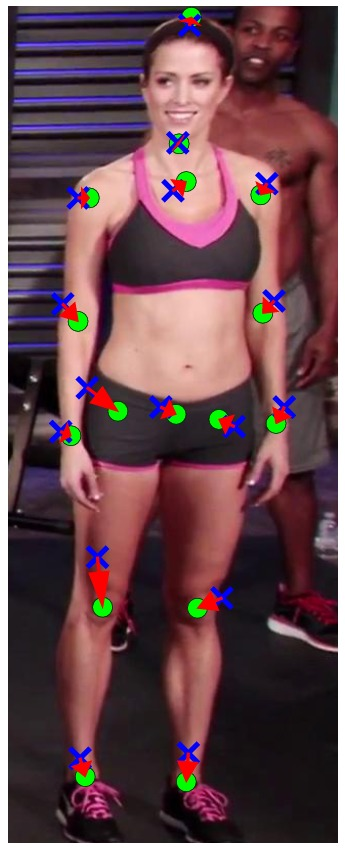
\includegraphics[height=.65\columnwidth]{resources/Annotation_Correction/MotivativeAnnotation/MPII}
        &
        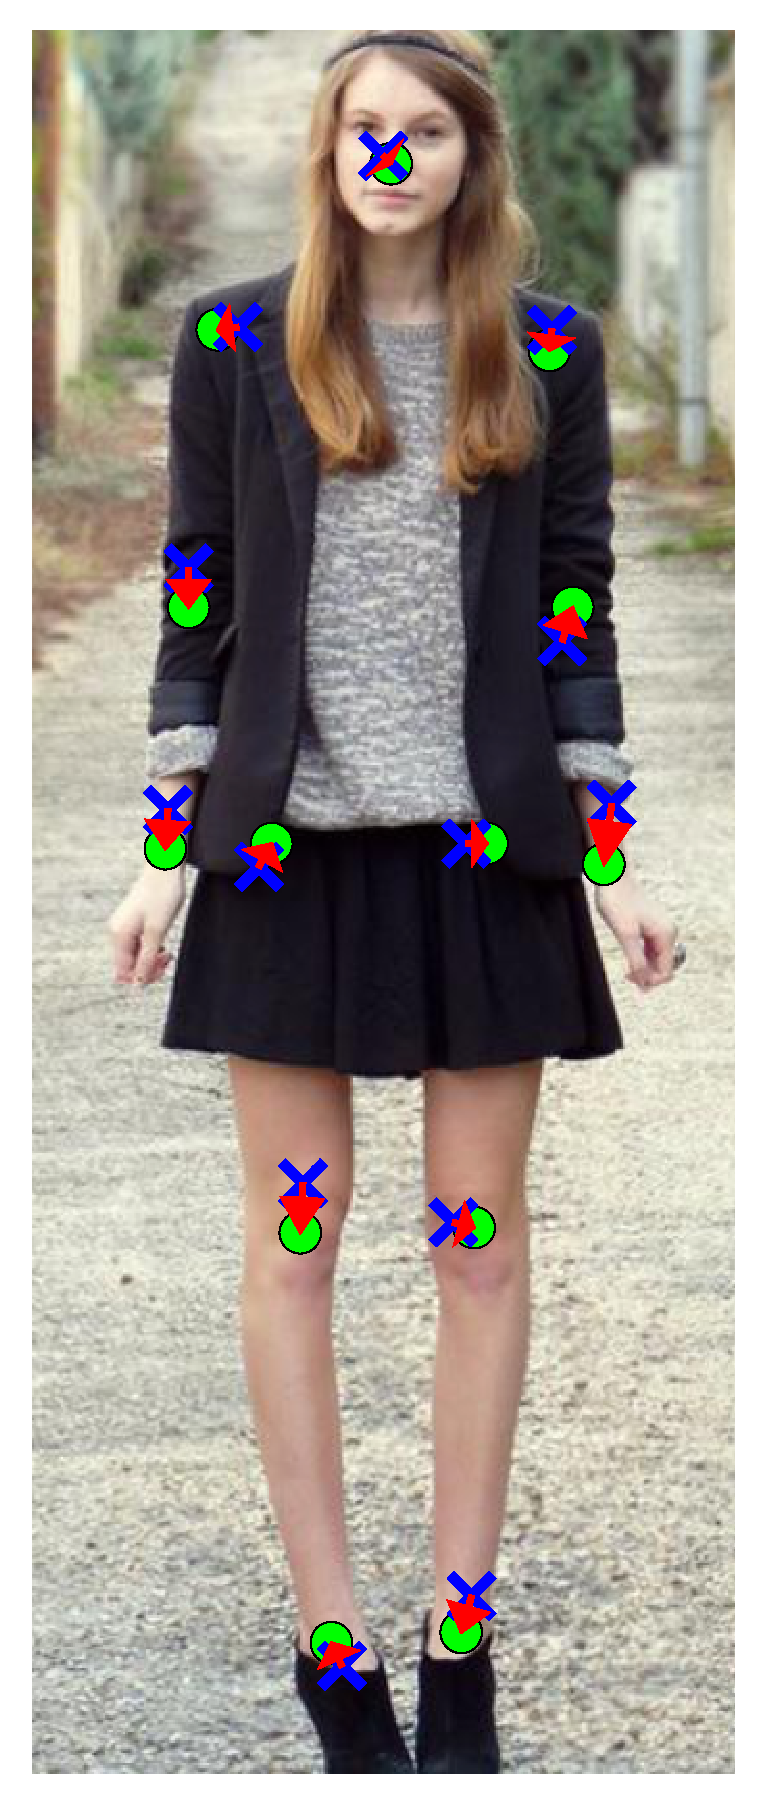
\includegraphics[height=.65\columnwidth]{resources/Annotation_Correction/MotivativeAnnotation/FashionPose}
        &
        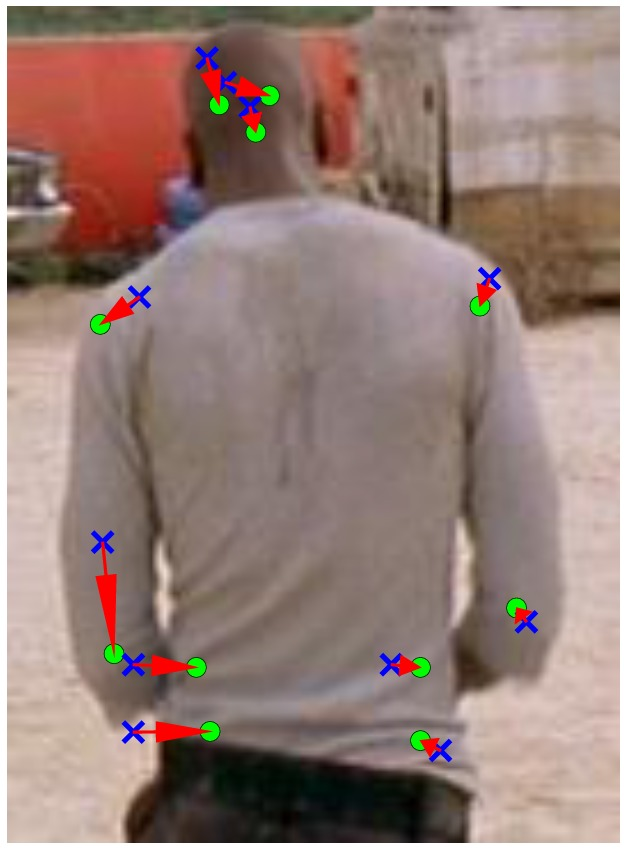
\includegraphics[trim=50 0 50 0,clip,height=.65\columnwidth]{resources/Annotation_Correction/MotivativeAnnotation/FLIC}
        \\
        (a) MPII
        &
        (b) Fashion
        &
        (c) F
        \end{tabular}
    \caption{Examples of inconsistent annotations of human pose among different datasets. \emph{Blue} markers denote the original annotations. The arrows and \emph{green} markers show the correct location at which the points should be annotated.}
    \label{fig:wrong_anno}
\end{figure} 
\begin{figure}[t!]
    \centering
    \begin{subfigure}{0.065\textwidth}
            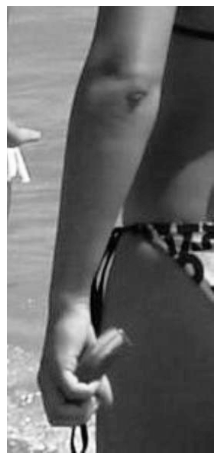
\includegraphics[height=2.55cm]{resources/Annotation_Correction/Fig_Intro/intro_2_0}
    \end{subfigure}
    \hfill
    \begin{subfigure}{0.065\textwidth}
            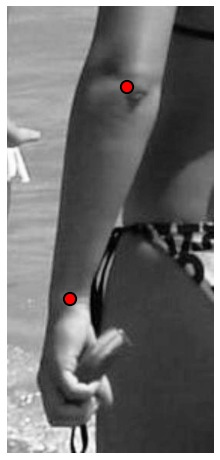
\includegraphics[height=2.55cm]{resources/Annotation_Correction/Fig_Intro/intro_2_1}
    \end{subfigure}
    \hfill
    \begin{subfigure}{0.065\textwidth}
            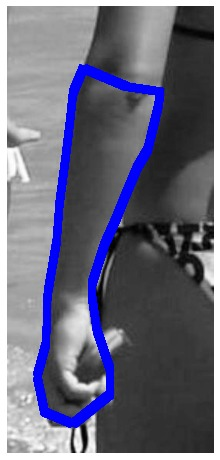
\includegraphics[height=2.55cm]{resources/Annotation_Correction/Fig_Intro/intro_2_2}
    \end{subfigure}
    \hfill
    \begin{subfigure}{0.085\textwidth}
            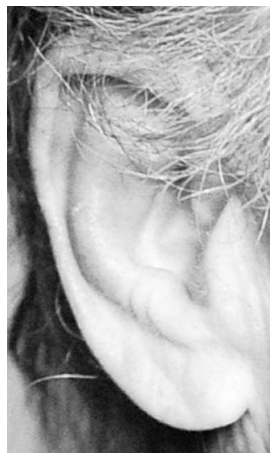
\includegraphics[height=2.55cm]{resources/Annotation_Correction/Fig_Intro/intro_1_0}
    \end{subfigure}
    \hfill
    \begin{subfigure}{0.085\textwidth}
            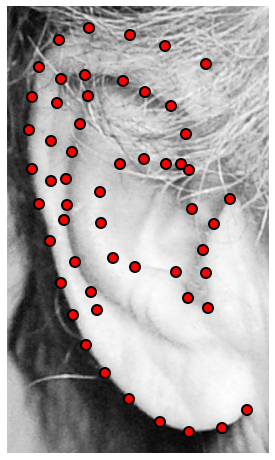
\includegraphics[height=2.55cm]{resources/Annotation_Correction/Fig_Intro/intro_1_1}
    \end{subfigure}
    \hfill
    \begin{subfigure}{0.085\textwidth}
            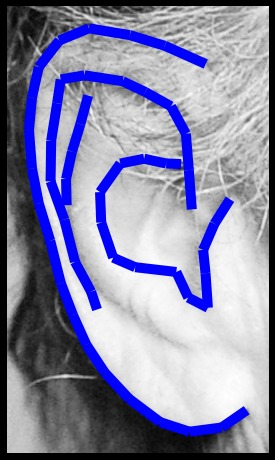
\includegraphics[height=2.55cm]{resources/Annotation_Correction/Fig_Intro/intro_1_2}
    \end{subfigure}
    \\
    \begin{subfigure}{0.156\textwidth}
            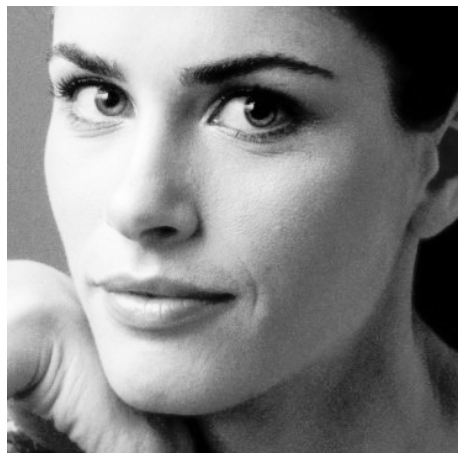
\includegraphics[height=2.8cm]{resources/Annotation_Correction/Fig_Intro/intro_0_0}
    \end{subfigure}
    \hfill
    \begin{subfigure}{0.156\textwidth}
            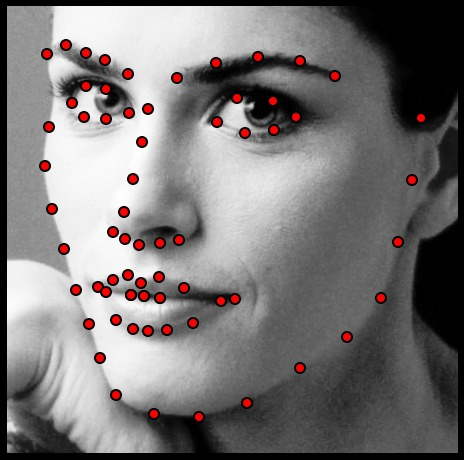
\includegraphics[height=2.8cm]{resources/Annotation_Correction/Fig_Intro/intro_0_1}
    \end{subfigure}
  	\hfill
    \begin{subfigure}{0.156\textwidth}
            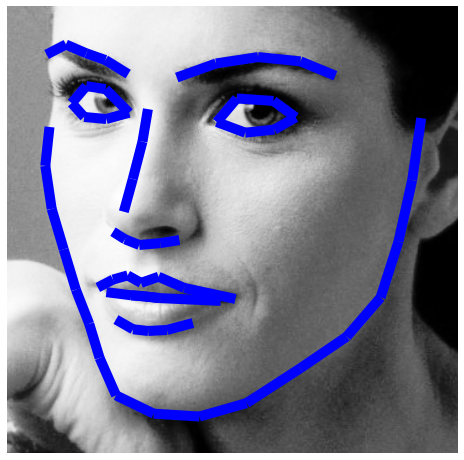
\includegraphics[height=2.8cm]{resources/Annotation_Correction/Fig_Intro/intro_0_2}
    \end{subfigure}
    \caption{Comparison of the standard landmark annotation (\emph{red} dots) with the curve annotation (\emph{blue} lines) on arms, ears and faces. It is evident that the curve annotations surpass the inevitable inconsistency of sparse annotations.}
    \label{fig:intro_annotation_correction}
\end{figure}


Statistical Deformable Models (SDMs) of various objects is a well-studied and popular area in the intersection of computer vision and machine learning \cite{Cootes1995, Cootes2001, Matthews2004, Saragih2011, Belhumeur2011, Zhu2012, Xiong2013}. Recently, we have witnessed tremendous developments on SDMs of human faces and bodies trained with images that are captured under unconstrained conditions, usually referred to as ``in-the-wild" \cite{Belhumeur2011, Cao2012, Zhu2012, Xiong2013, Asthana2013, Tzimiropoulos2014, Asthana2014, kazemi2014one, Alabort2014, zhu2015face, antonakos2015feature, antonakos2015active, Joan_cvpr2015, tzimiropoulos2015project}. This is attributed to:
\begin{itemize}
\item The abundance of complex visual data, spread through web services (e.g. Youtube, Flickr, Google Images), which has led to the development of ``in-the-wild" databases of human faces and bodies \cite{Belhumeur2011, Le2012, Zhu2012, Burgos2013}.

\item The manual annotation of such databases that has been undertaken by several research teams \cite{sagonas2016faces,charles2013domain,dantone2014body,andriluka14cvpr}.

\item The development of powerful visual features that are able to describe objects and their parts in a robust manner (e.g., SIFT \cite{lowe1999object}, HoGs \cite{Dalal2005}
%and Deep Convolutional Neural Networks \cite{sermanet2013overfeat}
), as well as generative and discriminative methodologies for learning SDMs.
\end{itemize}

However, there are two main drawbacks when building SDMs directly on manually annotated landmarks:
\begin{itemize}

\item Annotating with regards to consistent landmarks is an extremely time-consuming, tedious and labour intensive work \cite{sagonas_iccv_300w_2013}, which is usually performed by a trained person. Furthermore, for various object classes, it requires a highly skilled person in order to identify and annotate landmarks in a consistent manner. For example, the human ear has very complicated inner structures (helix, crus antihelicis, scapha, tragus, lobe etc.) which remarkably differ between different ears. Moreover, certain ear parts, such as fossa triangularies and crus helicis, do not appear in all ears and their visibility is highly sensitive to the head pose and illumination variation. Another such example is the human body, which is generally annotated with regards to a number of landmarks that intuitively correspond to a set of body joints. For most body pose databases, the annotation task was undertaken by a crowd-sourcing Internet marketplace, so-called Amazon Mechanical Turk (AMT). Unfortunately, this resulted in acquiring inconsistent and inaccurate annotations, in many cases\footnote{In the case of faces, the quality of annotations produced from AMT are extremely inaccurate and cannot, by any means, be compared with the ones provided by the recent 300W competition \cite{sagonas_iccv_300w_2013,sagonas2016faces}.} (please see Figure \ref{fig:wrong_anno}). As it was also recently pointed out \cite{tompson2015efficient}, the inconsistencies in body joint annotations may also render the comparison between different human pose estimation methodologies irrelevant.

\item The nature of many deformable objects does not allow them to be annotated with regards to a consistent set of landmarks (e.g., bottles, fruits etc.). Additionally, it is very difficult to consistently annotate the outline of certain objects such as faces, ears, body, since these landmarks do not have any semantic meaning. That is why many state-of-the-art methods opt to leave the boundary out when reporting results \cite{Tzimiropoulos2014, Asthana2014}. The majority of the state-of-the-art methods for model-based landmark localisation \cite{Cao2012, Zhu2012, Xiong2013, Tzimiropoulos2014, Asthana2014} are not applicable to objects with inconsistent sets of landmarks.

\end{itemize}

To illustrate how time-consuming careful annotation of a complex deformable object is, we lay down our own experience based on the human ear. A trained annotator needs an average of 4 minutes per image for the manual annotation of 55 landmarks. This means that the annotation of 1000 images requires a total of about 67 hours. Furthermore, the quality of training as well as fatigue greatly influence the annotation accuracy. Hence, a second pass on the annotated data is, in many cases, necessary. Due to the fact that manual annotation is a costly and labour-intensive procedure, unsupervised learning of deformable models for the task of object alignment has recently attracted some attention \cite{frey2003learning, baker2004automatic, cootes2004groupwise, jojic2006escaping, Huang2006, kokkinos2007unsupervised, jiang2009learning, liu2009simultaneous, Zhang2012}. However, because the problem of fully unsupervised discovery of the deformations of arbitrary objects is difficult and ill-posed, the limited number of methods that have been proposed for the task cannot be directly applied to arbitrary collections of ``in-the-wild" images. On the other hand, the method of \cite{antonakos2014automatic}, which can deal with ``in-the-wild" images, requires a set of consistently annotated sparse shapes to perform deformable face congealing.


\section{Contributions}

In this paper, we propose a solution for annotating an object with regards to its deformations that requires considerably less effort compared to manual annotation and, at the same time, can be used to define statistical deformations for objects without a consistent set of landmarks. We employ the proposed method in order to construct SDMs based on the outline of human body parts (i.e., arms and legs). The proposed SDM can also be used to provide accurate and consistent annotations for several of the body joints (such as wrist, elbow etc.).
To this end, we argue and empirically demonstrate that it is better to annotate an object with regards to a set of continuous lines that describe its shape. An example is provided in Figure \ref{fig:intro_annotation_correction}, which compares the standard landmark annotations that are employed in the current literature with the proposed curve annotations for arms, ears and faces. It becomes evident that the curve annotations avoid the inherent ambiguity of placing sparse landmarks and offer a richer description of the object's shape.
%
Furthermore, these curves can be automatically generated by recently proposed methods that perform discriminative segmentation of objects \cite{luo2013pedestrian,liu2015matching}.
%
Note that the work in~\cite{zuffi2012pictorial} is the only one that shows that training SDMs based on the outline contours of the human body parts has considerable advantages compared to using the sparse skeleton joints, as done by the majority of existing SDMs for human pose.

Furthermore, we capitalise on recent advances on multiframe optical flow estimation \cite{Garg:2013hu,tomasi2012dense,snape15faceflow} and show that the relevant methodologies have matured enough to densely annotate the proposed shapes using either simplistic or even more sophisticated and robust shape representation methods \cite{Nguyen2013}.
In particular, in order to build dense correspondences between different shape instances of the same object class, we jointly estimate the optical flow among all the instances by imposing low-rank constrains, an approach that we call \emph{Shape Flow}. Multiframe optical flow has originally been applied on video sequences, relying on the assumptions of colour consistency and motion smoothness \cite{Garg:2013hu}. However, these assumptions do not hold in our case, where we have a collection of shapes. Therefore, we introduce appropriate modifications based on the consistency of image-based shape representation, as well as low-rank priors.


Additionally, we show that the proposed methodology can be applied on landmark localisation, even though it is not tailored for that task, achieving particularly good performance. Specifically, we explain how to build powerful dense SDMs that are suitable for objects that have rich interior texture but lack landmarks consistency. Furthermore, we show how to build a powerful patch-based SDM on the sparse outline landmarks of objects that do not have semantically meaningful interior textures. Using the resulting outline patch-based SDM, we report state-of-the-art performance on the task of human body parts localisation on challenging databases. Finally, we show that the proposed patch-based SDM can be used to provide consistent annotations for different body parts.




In summary, the contributions of this paper are:
\begin{itemize}

  \item We propose one of the first, to the best of our knowledge, methodologies that constructs accurate SDMs from a set of training data with inconsistent annotations. We show that the proposed methodology tremendously reduces the manual workload thanks to the highly effective curve annotations.

  \item We illustrate the ability of the proposed method to generate consistent sparse landmark annotations for object classes which, by nature, make it impossible to be manually annotated in a consistent way.

  \item We show that it is more advantageous to model the human body parts (e.g. arms) with a set of sparse landmarks on their outline, rather than on their skeleton joints. This is because the outline landmarks, which can be acquired by our method in a straightforward way, exhibit better consistency compared to the inevitable inconsistency of the joint landmarks.

  \item We report state-of-the-art quantitative and qualitative results on human body parts localisation by employing a patch-based SDM trained on the outline landmarks that are sampled by the dense correspondences. Our proposed model outperforms all current state-of-the-art techniques that are trained on skeleton joints.

  \item We show that the employed patch-based SDM corrects the annotations that are currently provided for most major human body pose databases \footnote{\label{foot:annotations}The corrected annotations are publicly available in \url{http://www.ibug.doc.ic.ac.uk/resources/bodypose-anno-correction}.}.

\end{itemize}



%In our experiment, we show that building robust dense models trained with inconsistent annotation and %trained with curve annotation improves performance of discriminative models trained on carefully %annotated data including ears, faces, bottles, (cars ?) and bodies. Evaluation methods and choices are %described in details.




%We propose a framework to (1) construct SDMs using training data with inconsistent annotation, (2) %introduce highly effective curve annotation which tremendously reduces manual work overload but %maintains same performance level against state-of-the-art SDMs and (3) build dense correspondent SDMs %with shape flow.

%(1)
%Annotated data of same objects can have various number of landmarks, \cite{?} shown faces have %landmarks different in range 10+ to 70+. Building SDMs (e.g. Active Appearance Models), however, %%require training data are annotated consistently, for example, all faces have 68 landmarks, 6 landmarks %for an eye and 9 for a nose \cite{?}. Such property of SDMs largely limited their application area like %combining different dataset as one. We propose the pipeline with non-rigid alignment and support vector %shape to blend landmarks into relatively consistent shape discriminator before building models.

%(2)



%(3)


% Back Ground, uses Nondas' paper "Automatic Construction of Deformable Models In-The-Wild" as place holder
%The two most closely related works to the proposed
%method are the automatic construction of Active Appearance
%Models (AAMs) in \cite{?} and the so-called RASL
%methodology in \cite{?} for person-specific face alignment.
%There are two main differences between our framework
%and \cite{?}. (1) We use a predefined statistical shape model
%instead of trying to find both the shape and appearance models.
%We believe that with the current available optimization
%techniques, it is extremely difficult to simultaneously optimize
%for both the texture and shape parameters. (2) We
%employ the robust component analysis of \cite{?} for the appearance
%which deals with outliers. Thus, even though
%our method is similar in concept to \cite{?}, these two differences
%make the problem feasible to solve. In particular, the
%methodology in \cite{?} fails to create a generic model even in
%controlled recording conditions, due to extremely high dimensionality
%of the parameters to be found and to the sensitivity
%of the subspace method to outliers. This was probably
%one of the reasons why the authors demonstrate very
%limited and only person-specific experiments. Furthermore,
%our methodology bypasses some of the limitations of \cite{?},
%which requires the presence of only one low-rank subspace,
%hence it has been shown to work only for the case of congealing
%images of a single person. Finally, we argue that
%in order for an automatically constructed AAM methodology
%to be robust to both within-class and out-of-class outliers4,
%which cannot be avoided in totally unsupervised setting
%statistical component analysis techniques should be
%employed \cite{?}.


\begin{figure}[t!]
    \centering
        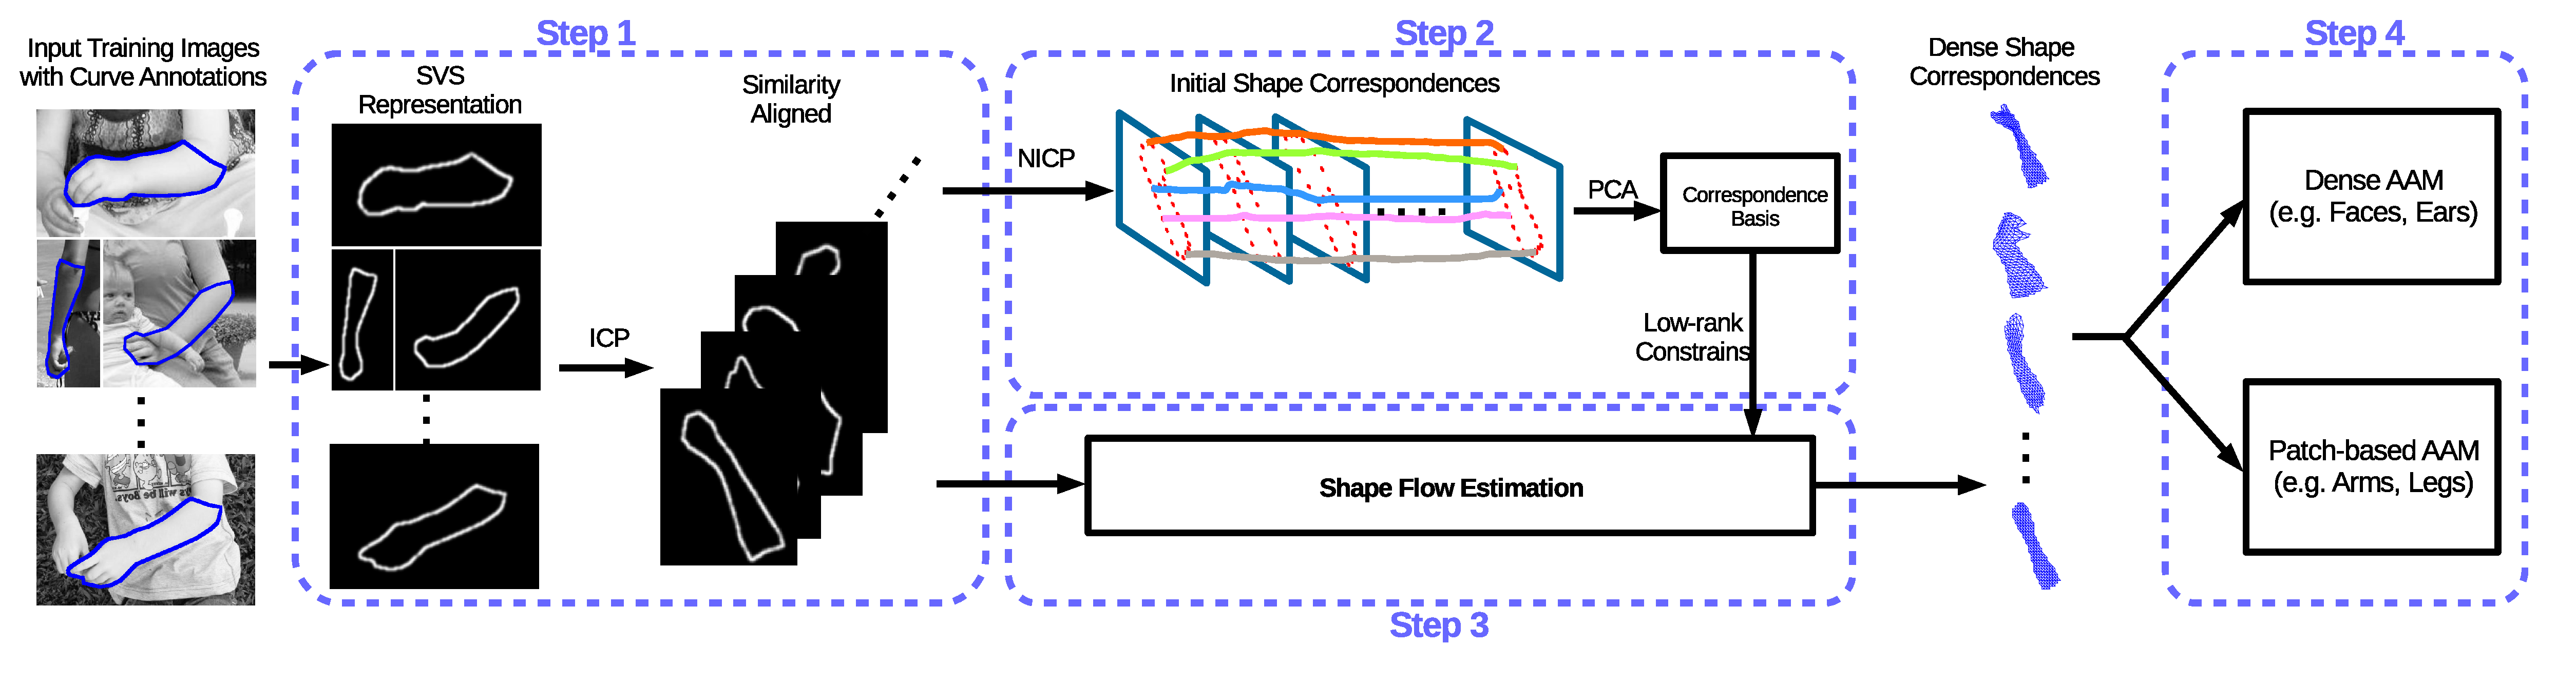
\includegraphics[width=\textwidth]{resources/Annotation_Correction/architecture3}
    \caption{Schematic description of the proposed pipeline. Figure best viewed by zooming in.}
    \label{fig:archi}
\end{figure}

\section{Constructing Deformable Models with Shape Flow}

% Deformable models are widely used for object detection, localization, recognition and tracking while training a deformable model with good generalisation requires tremendous amount of carefully annotated data, which is extremely time consuming. Even more, annotated data of a specific object category typically requires same numbers of landmarks for every training sample, making the annotation procedure significantly complex where corrext menual annotation of landmarks is impossible in various object classes e.g. ears.

% Despite the fact that that vast majority of existing methods are based on a sparse shape representation, dense shape representation reveals more nuanced structure in terms of [todo: explain].


This section presents the proposed method for establishing dense correspondences among training shapes
by only using curve annotations.
%
%We propose a novel framework for building deformable models that does not require any consistent set of annotated landmarks and is based on a dense shape representation. Our method only requires a set of point or curve line annotations that does not need to be consistent over different training samples.
%
%It combines the techniques of Non-rigid Iterative Closest Point (NICP) \cite{Amber2007}, multichannel Support Vector Shape (SVS) \cite{Nguyen2013} representation and multiimage subspace flow \cite{Garg:2013hu} in an effective framework that has significant descriptive power.
%
It takes as input a set of training images of a particular object class, along with the corresponding curve annotations. The steps of our pipeline, which are also depicted in Figure~\ref{fig:archi}, are the following:

\noindent\textbf{Step 1:} Represent the curve annotations in a consistent way using a multichannel extension of the Support Vector Shape (SVS) representation \cite{Nguyen2013}. Apply the Iterative Closest Point (ICP) algorithm \cite{Besl1992} to achieve an initial alignment of the SVS images.

\noindent\textbf{Step 2:} Construct a correspondence basis for the training SVS images. This is acquired by applying the Non-rigid ICP (NICP) algorithm of \cite{Amber2007} on the densely sampled annotated curves, followed by Principal Component Analysis (PCA).

\noindent\textbf{Step 3:} Establish dense correspondences between all the shapes in the training set by feeding the multichannel similarity-aligned SVS images into a multi-image subspace flow estimation.

\noindent\textbf{Step 4:} Utilise the dense correspondences acquired by the optical flow in order to automatically generate either dense or sparse (on the outline) landmark annotations, depending on the object class type. Then, build either a dense \cite{ramnath2008increasing, Amberg2009, anderson2014using} or a patch-based \cite{Tzimiropoulos2014} AAM, respectively.

The upcoming sections discuss each of the aforementioned steps in further detail.

%two major modules. The first module handles inconsistent annotation set by converting to landmark independent shape discriminator. While the other module produces shape flow on object discriminators to generate dense flow transformations in shape space following by robust PCA\cite{?} to generate deformable model. In this section, we present the entire architectures, design decision and algorithms.
\newcounter{steps}
{\refstepcounter{steps}\label{sec:step1}\subsection*{Step 1: Shape Representation Based on Support Vector Shapes}}
% \subsection{Shape Representation Based on Support Vector Shapes}
% \label{sec:step1}
%Ordinarily, construction of deformable model requires training data set having consistent number of landmarks. But unavoidable changes has to be made before applying same algorithm on diverse annotated data set.

In order to fully capture the variability among most deformable objects' shapes annotations, we use a representation based on SVS \cite{Nguyen2013}. An SVS is a decision function trained on shapes using Support Vector Machines (SVMs) with Radial Basis Function (RBF) kernels. In this way, a shape is represented as a classifier function, which has several advantages: (a)~the representation is completely generic, e.g. it can be applied to sparse landmark points, curves lines or a combination of the two, and~(b) it fuses inconsistent landmarks into consistent and directly comparable decision functions. Furthermore, this representation is also robust against noise, missing data and outliers \cite{Nguyen2013}.

%In practice, we assume that all the training images correspond to the same object category and contain a set of inconsistent points and curve line annotations.
The curve annotations for all training images are densely sampled to yield a set of landmarks per image, with this set being different for every training image. To train the SVM, these landmarks are assigned as belonging to the `positive' class, whereas randomly sampled points around them are assigned as belonging to the `negative' class. Since the positive class has far less points than the negative class, landmarks are assigned considerably larger weights so that $N_p \times W_p=N_n \times W_n$ where $N_p, N_n$ are number of points of the positive and negative class respectively and $W_p, W_n$ are their corresponding weights.

SVMs with RBF kernel functions map any number of data points onto an infinite-dimensional space where positive and negative points are linearly separable, hence the classification boundary on the 2D space represents the actual shape of the object.
%Note that the decision function for SVMs can be mathematically expressed as:
%\begin{equation} \label{eq:decisionfunc}
%    d(\bm{x})=\sum_i\alpha_i \, k(\bm{x}_i^*,\bm{x})
%\end{equation}
%where $\bm{x}_i^*$ are the so-called support vectors and \mbox{$k(\bm{x}, \bm{y}) = \exp(-{\|\bm{x} -\bm{y}\|^2}/{2 \sigma^2})$} is the RBF kernel.
Let $d(\bm{x})$ be the decision function for SVMs. In our formulation, $d(\bm{x})$ can be defined for every pixel $\bm{x}$ of the corresponding object image, therefore we interpret it as an image and we call it \emph{SVS image}.

%Figure~\ref{fig:archi} includes some exemplar SVS representations of arm shapes (Step 1 box)

%Figure \ref{fig:build_svs} shows an exemplar shape representation of the human ear using SVS. As it can be observed, the final result does not drastically depend on the original number of annotated landmarks.


% \begin{figure}[b!]
%     \centering
%     \begin{subfigure}[b]{0.2\textwidth}
%             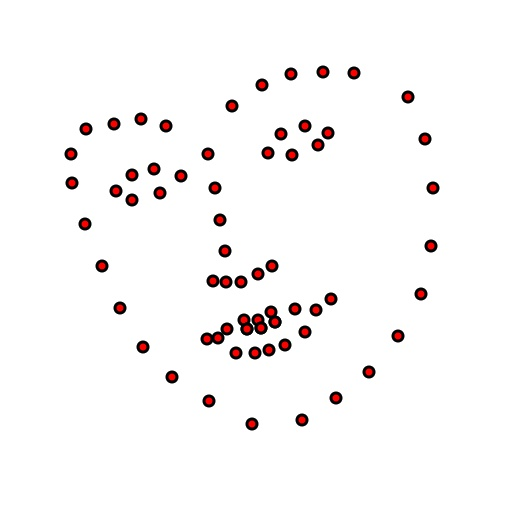
\includegraphics[width=\textwidth]{resources/Annotation_Correction/landmark}
%         \caption{Spare landmarks}
%     \end{subfigure}
%     \qquad
%     \begin{subfigure}[b]{0.2\textwidth}
%             
\includegraphics[width=\textwidth]{resources/Annotation_Correction/svs}
%         \caption{Decision function}
%         \label{fig:svs}
%     \end{subfigure}
%     \caption{Exemplar SVS shape representation. The decision function is trained on the set of sparse landmarks. In (b), brighter colour represents higher probability of a pixels belonging to the original shape.}
%     \label{fig:build_svs}
% \end{figure}

% \begin{figure}[b!]
%     \centering
%     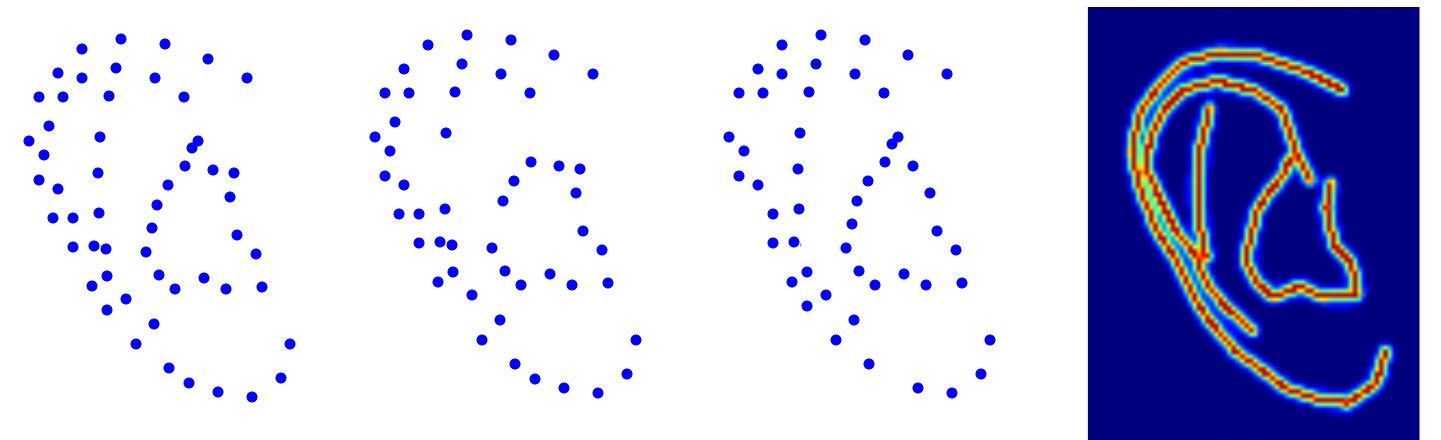
\includegraphics[width=0.4\textwidth]{resources/Annotation_Correction/svs2}
%     \caption{Exemplar SVS shape representation. A similar SVS image is obtained from different annotations of the same shape.}
%     \label{fig:build_svs}
% \end{figure}

We extend the SVS representation to support also the case where multiple curves with different labels are annotated. This is useful when annotating different structures of the same object, such as the left and right eyebrows on faces. Even though not absolutely necessary in our framework, it can provide further guidance on the estimation of dense shape correspondences for various object classes. In more detail, we create a multichannel SVS image $\bm{d}(\bm{x})=[d_1(\bm{x}) \cdots d_i(\bm{x}) \cdots d_{N_c}(\bm{x})]$, where $d_i(\bm{x})$ is the SVS image that corresponds to the curve annotation of the $i$-th structure and $N_c$ is the total number of structures (a single curve annotation is the special case where $N_c=1$). Note that we do not necessarily require that all structures are annotated in all the object images: in the case that a structure is not annotated, the corresponding channel of the SVS image simply takes a zero value for all pixels. The shape flow estimation can deal with such missing information thanks to the spatial regularization and the low-rank constraint that it adopts, c.f.~Step~\ref{sec:step3}.

After constructing the SVS representation for all images, the next step is to apply a simple similarity alignment over them. This is done because the goal here is to build a model capable of effectively representing non-rigid local shape deformations rather than global rotation, translation and scaling. The alignment is performed by using the ICP algorithm \cite{Besl1992} on the annotated landmarks point cloud of the training images.


%\subsection{Correspondence Basis for Shape Flow Estimation}
{\refstepcounter{steps}\label{sec:step2}\subsection*{Step 2: Correspondence Basis for Shape Flow Estimation}}

We define the problem of shape flow as the joint estimation of optical flow fields between a reference SVS image and every SVS image of the training dataset, which yields dense correspondences across SVS images. This also defines for every training SVS image a warping function that registers it with the reference SVS image. To establish the dense correspondences robustly, we are inspired by the idea of subspace constraints in the estimation of multiframe optical flow \cite{Garg:2013hu,tomasi2012dense,snape15faceflow}.

Instead of the \emph{motion} basis used in multiframe optical flow formulation of \cite{Garg:2013hu}, we build a \emph{correspondence} basis that introduces constraints on how points of different shapes are matched to each other. Every pixel of the reference SVS image is matched to its corresponding position at every training SVS image and in this way defines a \emph{correspondence vector}. This vector consists of the 2D locations of the specific point in all SVS images. To form this vector, the training images are arranged in an arbitrary order. Similarly to the order of the training samples when PCA is applied, this order does not affect the result of our method and any re-ordering would produce exactly the same results.


Formally, let $N_t$ be the number of training SVS images and $n=1,\dots,N_t$ be the training image index. Also, let $\bm{q}_1(n),\dots,\bm{q}_R(n):\{ 1,\dots,N_t \} \rightarrow R^2$ be the $R$ orthonormal elements of the correspondence basis, where $\bm{q}_i(n)$ is the displacement vector that matches the points of the reference SVS image with the points of the $n$-th training SVS image, according to the variation described from the $i$-th correspondence basis element. Note that the basis elements $\bm{q}_i(n)$ are independent from the point location. Note also that the number of basis elements is typically much smaller than the full dimensionality ($2 N_t$) of correspondence vectors, therefore this basis plays a role of dimensionality reduction. 

In addition, let $\Omega \subset R^2$ be the image domain of the SVS images and $\bx$ denote the point location. We denote the shape flow result as $\bm{u}_n(\bx):\Omega\times \{1,\dots,N_t\} \rightarrow R^2$,  where $\bm{u}_n(\bx)$ is the displacement vector that matches the point $\bx$ of the reference SVS image with its corresponding location at the $n$-th training SVS image.

Using the constructed correspondence basis, the shape flow can be approximated as:
\begin{equation}\label{eq:LinTrajModel}
    \bm{u}_n(\bx) \approx
    \textstyle \, \sum_{i=1}^R \, \bm{q}_i(n)v_i(\bx) \,\, ,
\end{equation}
where $v_i(\bx)$ is the weight that needs to be applied on the $i$-th correspondence basis element, in order to get the correspondence vector for the point location $\bm{x}$. In other words, the shape flow for every point $\bm{x}$ is described as a linear combination of basis elements that is controlled by the coefficients $v_i(\bm{x})$.
The values of the $i$-th coefficient for all the points $v_i(\bm{x})$ can be interpreted as an image defined on $\Omega$. Using the correspondence basis, the determination of the shape flow boils down to the determination of the set of coefficients $v_i(\bm{x})$. The above representation of shape flow, constrains the correspondence vectors to lie on a subspace and, therefore, acts as a low-rank prior that enforces coherency of the shape registration result over the whole training dataset of shapes.


To effectively build the correspondence basis, we first transform the original annotations to sparse point clouds. Then, we apply the NICP algorithm of \cite{Amber2007} between the point cloud of annotations in the reference shape and the one of every shape of the training set. NICP iteratively deforms the cloud of points of every shape to match the points of the reference shape. This yields an initial estimation of the correspondence vectors on the sparse locations of annotated landmarks on the reference shape. Finally, the correspondence basis is found by applying PCA on these correspondence vectors and keeping only the first $R$ principal components.



% For all dense transformations $\bm{u}_n(\bm{x}), n \in \{1,...,F\}$, where $F$ is number of data and $\bm{x}$ is vector of pixels, Principle Component Analysis (PCA) is performed on trajectory to obtain low rank trajectory basis:
% \begin{equation}
%     \begin{bmatrix}
%         \bm{u_1}(\bm{x}) \\
%         \vdots \\
%         \bm{u_F}(\bm{x})
%     \end{bmatrix}
%     =
%     \begin{bmatrix}
%         \bm{q_1}(1) & \cdots & \bm{q_R}(1) \\
%         \vdots      & \ddots & \vdots  \\
%         \bm{q_1}(F) & \cdots & \bm{q_R}(F)
%     \end{bmatrix}
%     \times
%     \begin{bmatrix}
%         \bm{v_1}(x) \\
%         \vdots \\
%         \bm{v_R}(x)
%     \end{bmatrix}
% \end{equation}
% where $\bm{q_i}(n)$ are low rank components with $R \ll 2F$ and $\bm{v_i}(x)$ weighted each component with dependencies on $x$. Simpler expression shown below:
% \begin{equation}
%     \bm{u}_n(\bm{x})=\sum_{i=1}^R\bm{q_i}(n)\bm{v_i}(x)+\bm{\varepsilon_n}(\bm{x})
% \end{equation}

\begin{figure}[t!]
    \centering
    \newcommand{\flowh}{0.25\columnwidth}
    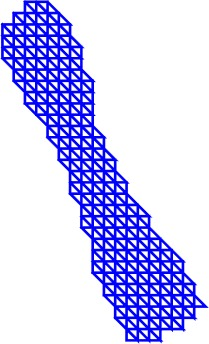
\includegraphics[height=\flowh]{resources/Annotation_Correction/Fig_Flows/1}
    \includegraphics[height=\flowh]{resources/Annotation_Correction/Fig_Flows/2}
    \includegraphics[height=\flowh]{resources/Annotation_Correction/Fig_Flows/3}
    \includegraphics[height=\flowh]{resources/Annotation_Correction/Fig_Flows/4}
    \includegraphics[height=\flowh]{resources/Annotation_Correction/Fig_Flows/5}
    \includegraphics[height=\flowh]{resources/Annotation_Correction/Fig_Flows/6}
    \caption{Exemplar deformation fields for the left arm, obtained using the proposed pipeline. Figure best viewed by zooming in.}
    \label{fig:deformationfield}
\end{figure}

\begin{figure}[b!]
    \centering
    \includegraphics[width=0.9\columnwidth]{resources/Annotation_Correction/models}
    \caption{Dense shape models build for faces and ears. Dense shapes are presented as grid for better visualization.}
    \label{fig:dense_models}
\end{figure}




% ---------------------------------------------------------------------------------------------------------------------------------------------------
{\refstepcounter{steps}\label{sec:step3}\subsection*{Step 3: Shape Flow Estimation}}
% \subsection{Shape Flow Estimation}
% \label{sec:step3}


%Using the SVS functions built from training data, one of the main steps of our pipeline is to estimate dense correspondences between all these functions. We propose to perform this estimation simultaneously for all training data, by using the correspondence basis.

As already mentioned, our shape flow estimation builds upon robust methods for multiframe optical flow estimation \cite{Garg:2013hu}. However, optical flow estimation typically works based on the assumptions of brightness or colour constancy and motion smoothness, whereas in our setting the input training data correspond to shapes. For this reason, we propose to modify the formulation of \cite{Garg:2013hu} by using the correspondence basis that we introduced in conjunction with the SVS representation of shapes.


%
%In order to learn the such a subspace, we first transform the original annotation to point clouds. Then, we use NICP to align the previous point clouds with respect to a reference point cloud template. NICP iteratively deforms each point cloud until its points match the ones on the shape template and correspondences are established. However, because optical flow is a pixel-wise frame registration technique, we need to establish correspondences for all pixels on the reference frame rather than for sparse point clouds. To achieve this, we apply Thin Plate Spline (TPS) \cite{Bookstein1989} to find correspondences for all pixels in the reference frame given the point cloud correspondences provided by the previous NICP stage. Once dense correspondences have been established among all pixels, the so-called correspondence subspace is obtained by performing PCA the trajectory of all pixels. Note that incorporating the previous subspace as a low rank constrained in optical flow is consistent with its assumption of smooth motion.


Let $\bm{d}(\bx\;n)$, $\bm{d}(\bx\;0):\Omega\rightarrow R^{N_c}$ be the $n$-th training SVS image and the reference SVS image respectively. Following \cite{Garg:2013hu}, we propose to estimate the shape flow over all training images by minimizing the following energy:
\begin{align}
E_{sf} & =\alpha
\int_{\Omega}\sum_{n=1}^{N_t} \|\bm{d}(\bx+\bm{u}_n(x);n)-\bm{d}(x;0)\| \ud \bx \label{eq:costfunc}\\
    &+ \beta \int_{\Omega}\sum_{n=1}^{N_t}\|\bm{u}_n(\bx)-\sum_{i=1}^R\bm{q}_i(n)v_i(\bx)\|^2 \ud \bx \label{eq:lowrank}\\
    &+
\int_\Omega  \sum_{i=1}^R \,\, \left \|    \nabla v_i(\bx)    \right \|  \,\ud \bx \label{eq:TVterm}
\end{align}
This energy consists of two sets of unknown shape flows that are relatively close to each other: (i) $\bm{u}_n(x)$ which tries to explain the data from the input SVS images, and (ii) the shape flow determined by the correspondence basis coefficients $v_i(\bx)$ that are spatially regularised and enforce a low-rank prior.
%We minimize this energy jointly with respect to $\bm{u}_n(\bx)$ and $v_i(\bx)$.
%The positive parameters $\alpha$ and $\beta$ weigh the balance between the terms of the energy.


The \textbf{first term} of the above energy \eqref{eq:costfunc} is a data attachment term
that uses the robust $\Lone$-norm.  It is based on the assumption that the values of the reference SVS image $\bm{d}_0(\bx)$ at every pixel $\bx$ are preserved at its corresponding locations on all training SVS images $\bm{d}_n(\bx)$. The use of an $\Lone$-norm improves the robustness of the method since it allows deviations from this assumption, which might occur in practice.
The \textbf{second term} of the energy \eqref{eq:lowrank} penalizes the difference between the two sets  of shape flows and acts as a coupling term between them.
The \textbf{third term} of the energy \eqref{eq:TVterm} corresponds to the spatial Total Variation regularization \cite{rudin92} of
the correspondence basis coefficients $v_i(\bx)$.
This term penalizes spatial oscillations of each coefficient caused by distortions of the SVS images but not strong discontinuities that are desirable in the borders of different object regions. In addition, this term allows to fill in information into regions where the shape information in the SVS images is missing, due to e.g.~regions with no annotations.

We implement the minimization of the energy $E_{sf}$ by using the optimization algorithm described in \cite{Garg:2013hu}. For more details, please refer to the Supplementary Material.
%We slightly modify this algorithm so that, instead of initialising the coarse-to-fine and warping iterations with a zero flow, we use Thin Plate %Splines (TPS) \cite{Bookstein1989} interpolation of the initial correspondence vectors described in Step~\ref{sec:step2}.
%This yields a significantly better initial location of the highly-nonconvex objective function and improves the computational efficiency, since much less coarse-to-fine pyramids are needed.
%
Figure~\ref{fig:deformationfield} shows some examples of deformation fields derived from the estimated shape flow computed by the aforementioned method. These results correspond to exemplar training shapes in the case of an arm dataset. We observe that the shape flow estimation captures the shape and deformations of the human arm in a plausible way.

%In every coarse-to-fine and warping iteration, we use an initialization that comes from the previous iteration and for the very beginning, we initialize with a Thin Plate Splines (TPS) \cite{Bookstein1989} interpolation of the initial correspondence vectors described in Sec.~\ref{sec:step2}. We approximate the data term \eqref{eq:costfunc} by linearizing the SVS images around the initialization. After that, the energy becomes convex and we optimize it using alternating optimization w.r.t.~$v_i(\bx)$ and $\bm{u}_n(\bx)$. The minimization w.r.t.~
%$v_i(\bx)$ is decoupled for every coefficient $i$ and corresponds to Rudin-Osher-Fatemi Total Variation denoising \cite{rudin92}, which we solve efficiently by applying the first order primal-dual algorithm of \cite{Chambolle:Pock:JMIV2011}. The minimization w.r.t.~
%$\bm{u}_n(x)$ is decoupled for every pixel $\bx$ and every shape index $i$. This minimization is also implemented by applying the efficient primal-dual algorithm of \cite{Chambolle:Pock:JMIV2011}.






%
%
%To register all decision functions to temp`late shape, decision function $d_i(\bm{x}), i \in {1,...,F}$ are grouped into one sequence before applying flow algorithm. The objective cost function we would like to minimise is:
%\begin{align}
%    \operatorname*{arg\,min}_{\bm{u}_n(\bm{x}), \bm{v}}&=\alpha \int_{\Omega}\sum_{n=1}^F|\bm{d_n}(x+\bm{u}_n(x))-\bm{d_0}(x)\| dx  \label{eq:costfunc}\\
%    &+ \beta \int_{\Omega}\sum_{n=1}^F\|\bm{u}_n(x)-\sum_{i=1}^R\bm{q_i}(n)\bm{v_i}(x)\|^2 dx \label{eq:lowrank}\\
%    &+ \sum[\bm{TV}(Qv)]
%\end{align}
%where $d_n(x)$ is the decision function from~\eqref{eq:decisionfunc}, which returns possibilities of given coordinate classified as shape component where coordinates are from set $\Omega \in \Re^2$. $TV(Qv)$ is total variation as regularization on low rank subspace, $Q$ is trajectory basis and $v^T.L.v$ is low rank spacial constrains.
%
%Term~\eqref{eq:costfunc} state the shape constancy where points having similar classification probability are from same object.
%Part~\eqref{eq:lowrank} applies constrain on low rank trajectory basis states in section~\ref{sec:trabasis}.
%The objective cost function has two free parameters $u$ and $v$, so we perform alternating minimisation. The equation can be solved using a thresholding scheme after linearisation of image functions. The minimisation can be speed up by paralleling the minimisation for every spatial-temporal point $(x;n), x \in \Omega, n \in \{1,...F\}$ independently.
%
%
%
%
%
%
%After solving the equation, $\bm{u}_n(\bm{x}), x \in \Omega$ gives a group of deformation fields that registering every decision functions in the shape sequence to reference frame e.g. $\bm{u_1}(\bm{x})$ registers decision function $\bm{d_1}(\bm{x})$ to the reference frame. Figure~\ref{fig:deformationfield} demonstrates deformation fields that warps from reference frame where there is no deformation.

% \begin{figure}[ht]
%     \centering
%         \includegraphics[width=0.5\textwidth]{resources/Annotation_Correction/df}
%     \caption{Deformation field built}
%     \label{fig:deformationfield}
% \end{figure}



% Applying PCA on deformations trains dense deformable shape model:
% \begin{equation*}
%     \bm{s_p}=\bm{\bar{s}} + \bm{U}_s\bm{p}
% \end{equation*}
% where $\bm{s_p}$ is deformed shape instance. $\bm{\bar{s}}$ is mean shape and $\bm{U}_s\bm{p}$ are eigenvectors with corresponding parameters $p$. Figure~\ref{fig:models} shows an instance of deformed shape and appearance model.
% \begin{figure}[ht]
%     \centering
%     \begin{subfigure}[b]{0.22\textwidth}
%             \includegraphics[width=\textwidth]{resources/Annotation_Correction/Fig_dAAM/of_shape}
%     \end{subfigure}
%   	\hfill
%     \begin{subfigure}[b]{0.22\textwidth}
%             \includegraphics[width=\textwidth]{resources/Annotation_Correction/Fig_dAAM/of_app}
%     \end{subfigure}
%     \caption{Dense Deformable Model}
%     \label{fig:models}
% \end{figure}

% \begin{figure}[ht]
%     \centering
%     \begin{subfigure}[b]{0.22\textwidth}
%             \includegraphics[width=\textwidth]{resources/Annotation_Correction/Fig_dAAM/of_shape}
%     \end{subfigure}
%   	\hfill
%     \begin{subfigure}[b]{0.22\textwidth}
%             \includegraphics[width=\textwidth]{resources/Annotation_Correction/Fig_dAAM/of_app}
%     \end{subfigure}
%     \caption{Dense Deformable Model}
%     \label{fig:models}
% \end{figure}

{\refstepcounter{steps}\label{sec:step4}\subsection*{Step 4: Dense and Patch-Based Deformable Models}}
% \subsection{Dense and Patch-Based Active Appearance Models}





The deformation fields obtained from Step~\ref{sec:step3} can be used to naturally build two different kinds of effective Active Appearance Models (AAMs) \cite{Cootes2001, Matthews2004}: \emph{dense} \cite{ramnath2008increasing, Amberg2009, anderson2014using} and \emph{patch-based} \cite{Tzimiropoulos2014}. The only difference between these two AAM formulations is on the way that the shape is represented and, thus, the manner in which the texture is sampled. Each one of them is suitable for object classes with specific properties. The dense AAM provides an exceptionally effective modeling and fitting for non-articulated objects, such as ears and faces, whose appearance has characteristic structures that spread all over their region (even if these structures cannot be consistently annotated). On the other hand, there exist other challenging object classes, such as arms and legs, that not only cannot be consistently annotated with landmarks, but their appearance is distinctive only on the object's outline and not in its interior region. Especially in the case of human body parts, they are almost always covered by clothes, which makes it impossible to construct robust texture models.

\paragraph{Dense Active Appearance Model} Since all the deformation fields acquired by Step~\ref{sec:step3} are defined for the pixels of the reference SVS image, the spatial positions $\bm{x}_i=(x_i, y_i)$ of these pixels can be treated as point landmarks and the deformation fields as dense annotations of the object's shape. Consequently, building a dense shape model reduces to normalising these dense annotations with respect to a global similarity transform (typically using Procrustes Analysis) and applying PCA. A shape instance can be generated by the resulting shape model as:
\begin{equation}
    \bm{s}(\bm{p}) = \bm{\bar{s}} + \bm{S} \bm{p}
    \label{eq:shape_model}
\end{equation}
where $\bm{\bar{s}}$ is mean shape, and $\bm{S}$ and $\bm{p}$ are the shape bases and shape parameters, respectively.

By making explicit use of the one-to-one correspondence between pixels on the reference frame and on the deformation fields, the motion model of sparse holistic AAMs \cite{Cootes2001, Matthews2004} (piece-wise affine, thin-plates splines \cite{Bookstein1989}) is replaced by sampling all pixel values onto the reference frame. Let us define this sampling function, given a shape instance $\bm{s}(\bm{p})$, as $\mathcal{W}(\bm{s}(\bm{p}))$. Once the images have been warped, the texture model is obtained by applying PCA on them. A texture instance can be generated as:
\begin{equation}
    \bm{t}(\bm{c}) = \bm{\bar{t}} + \bm{T} \bm{c}
	\label{eq:tex_model}
\end{equation}
where $\bm{t}$ is the mean texture, and $\bm{T}$ and $\bm{c}$ are the texture bases and texture parameters, respectively.

Given a test image $\mathbf{I}$, the fitting process involves the minimization of the following cost function:
\begin{equation}
    \arg\min_{\bm{p}, \bm{c}}\|\bm{I}(\mathcal{W}(\bm{s}(\bm{p}))) - \bm{t}(\bm{c})\|_2^2
	\label{eq:aam_cost}
\end{equation}
This optimization problem is typically solved using the inverse-compositional Gauss-Newton algorithm, for which different variations have been proposed \cite{Matthews2004, Papandreou2008, Amberg2009, Tzimiropoulos2013, Alabort2014}. Note that the existence of the sampling function $\mathcal{W}()$ instead of a non-linear warping function has the advantage that all existing efficient gradient descent algorithms become exact.

\paragraph{Outline Patch-Based Active Appearance Model (PAAM)} The object classes for which the interior appearance does not have specific structure are modeled using patch-based AAMs \cite{Tzimiropoulos2014} trained on a set of sparse landmarks. Especially for human body parts (arms, legs), we strongly believe that the points located to the outline of the object are more suitable compared to the internal ones that correspond to the skeleton joints, which are commonly used by current literature \cite{buehler2011upper,charles2013domain,pfister2015flowing,yang2013articulated}.

The main differences between the patch-based and dense AAMs are that (a)~the densified shape instances are sub-sampled to include only the outline points, and (b)~the texture representation involves the sampling a neighbourhood around each point instead of a single pixel. Specifically, in order to build the outline sparse shape model, we simply select the outline points on the SVS reference frame. Then, by taking advantage of the dense correspondences obtained by Step \ref{sec:step3}, the shape model is trained in a similar way as in the dense case. Moreover, similar to the dense case, the texture model is built by sampling the image values from the sparse shape locations, i.e. $\mathcal{W}(\bm{s}(\bm{p}))$. However, contrary to dense AAMs, we sample a patch that is centred around each landmark point. These patches are then vectorised and concatenated in a single texture vector. Note that the optimization process remains exactly the same.


\section{Experimental Evaluation}

We evaluate the performance of the proposed methodology for the task of human body pose correspondence estimation, as well as non-rigid alignment ``in-the-wild''. For further experimental results, please refer to the supplementary material. Note that all steps of the proposed pipeline were implemented using the Menpo Project~\cite{menpo14}.

%Results of quantitative and qualitative evaluations are reported.

\begin{figure}[t!]
    \centering
    \includegraphics[width=\columnwidth]{resources/Annotation_Correction/Fig_Variance/final}
    \caption{Example of human pose annotation for left arm among 4 annotators. The large variance highlights the difficulty of obtaining consistent landmarks.}
    \label{fig:variance}
\end{figure}

\begin{figure}[!t]
    \newcommand{\fh}{0.24\columnwidth}
    \centering
    \includegraphics[height=\fh]{resources/Annotation_Correction/Fixing/fix_1}
    \hfill
    \includegraphics[height=\fh]{resources/Annotation_Correction/Fixing/fix_2}
    \hfill
    \includegraphics[height=\fh]{resources/Annotation_Correction/Fixing/fix_3}
    \hfill
    \includegraphics[height=\fh]{resources/Annotation_Correction/Fixing/fix_5}
    \hfill
    \includegraphics[height=\fh]{resources/Annotation_Correction/Fixing/fix_6}
    \hfill
    \includegraphics[height=\fh]{resources/Annotation_Correction/Fixing/fix_7}
    \hfill
    \includegraphics[height=\fh]{resources/Annotation_Correction/Fixing/fix_8}
    \hfill
    \includegraphics[height=\fh]{resources/Annotation_Correction/Fixing/fix_9}
    \hfill
    \includegraphics[height=\fh]{resources/Annotation_Correction/Fixing/fix_10}
    \hfill
    \includegraphics[height=\fh]{resources/Annotation_Correction/Fixing/fix_20}
    \hfill
    \includegraphics[height=\fh]{resources/Annotation_Correction/Fixing/fix_12}
    \hfill
    \includegraphics[height=\fh]{resources/Annotation_Correction/Fixing/fix_13}
    \hfill
    \includegraphics[height=\fh]{resources/Annotation_Correction/Fixing/fix_14}
    \hfill
    \includegraphics[height=\fh]{resources/Annotation_Correction/Fixing/fix_15}
    \hfill
    \includegraphics[height=\fh]{resources/Annotation_Correction/Fixing/fix_17}
    \hfill
    \includegraphics[height=\fh]{resources/Annotation_Correction/Fixing/fix_18}
    \caption{Demonstration of annotation correction using our method for the experiment of Section \ref{exp:qualitative}. \emph{Red} dots refer to officially provided landmarks, and \emph{green} dots are corrected position.}
    \label{fig:qualitative_anno}
\end{figure}

\begin{figure}[!t]
    \newcommand{\ofh}{0.24\columnwidth}
    \centering
    \includegraphics[height=\ofh]{resources/Annotation_Correction/Fittings/20.eps}
    \hfill
    \includegraphics[height=\ofh]{resources/Annotation_Correction/Fittings/3.eps}
    \hfill
    \includegraphics[height=\ofh]{resources/Annotation_Correction/Fittings/19.eps}
    \hfill
    \includegraphics[height=\ofh]{resources/Annotation_Correction/Fittings/4.eps}
    \hfill
    \includegraphics[height=\ofh]{resources/Annotation_Correction/Fittings/6.eps}
    \hfill
    \includegraphics[height=\ofh]{resources/Annotation_Correction/Fittings/15.eps}
    \hfill
    \includegraphics[height=\ofh]{resources/Annotation_Correction/Fittings/7.eps}
    \hfill
    \includegraphics[height=\ofh]{resources/Annotation_Correction/Fittings/8.eps}
    \hfill
    \includegraphics[height=\ofh]{resources/Annotation_Correction/Fittings/13.eps}
    \hfill
    \includegraphics[height=\ofh]{resources/Annotation_Correction/Fittings/17.eps}
    \\
    \includegraphics[height=\ofh]{resources/Annotation_Correction/Fittings/21.eps}
    \hfill
    \includegraphics[height=\ofh]{resources/Annotation_Correction/Fittings/23.eps}
    \hfill
    \includegraphics[height=\ofh]{resources/Annotation_Correction/Fittings/25.eps}
    \hfill
    \includegraphics[height=\ofh]{resources/Annotation_Correction/Fittings/27.eps}
    \hfill
    \includegraphics[height=\ofh]{resources/Annotation_Correction/Fittings/29.eps}
    \hfill
    \includegraphics[height=\ofh]{resources/Annotation_Correction/Fittings/31.eps}
    \hfill
    \includegraphics[height=\ofh]{resources/Annotation_Correction/Fittings/33.eps}
    \hfill
    \includegraphics[height=\ofh]{resources/Annotation_Correction/Fittings/35.eps}
    \hfill
    \includegraphics[height=\ofh]{resources/Annotation_Correction/Fittings/36.eps}
    \hfill
    \includegraphics[height=\ofh]{resources/Annotation_Correction/Fittings/37.eps}
    \hfill
    \includegraphics[height=\ofh]{resources/Annotation_Correction/Fittings/38.eps}
    \hfill
    \includegraphics[height=\ofh]{resources/Annotation_Correction/Fittings/39.eps}
    \caption{Demonstration of outline fitting of patch-based AAM on arms.}
    \label{fig:outline_fitting}
\end{figure}




\subsection{Non-rigid Object Alignment In-the-Wild}
\label{exp:daam_benchmark}
Herein, we compare the fitting accuracy of the dAAMs that are trained with our proposed framework with holistic sparse AAMs~\cite{Cootes2001,Matthews2004,antonakos2015feature}. We consider two object classes that demonstrate rich texture: face and ear.

\noindent\textbf{Databases \& Error Metrics} In the case of face, we trained both models using the 811 training images of the Labelled Faces Parts in-the-Wild (LFPW)~\cite{belhumeur2013localizing}. Sparse AAMs were built from the 68 points annotations provided by~\cite{sagonas_iccv_300w_2013,sagonas2016faces}. Our dAAMs were built as described in Step~\ref{sec:step4}. In both cases, the appearance is represented using pixel intensities. The results are reported on the 224 images of the LFPW testset. The fitting error is evaluated as the point-to-point distance normalised by the face's size, as proposed in~\cite{Zhu2012}.

In the case of human ear, given the lack of publicly available annotated databases, we collected 605 high resolution images captured under unconstrained conditions from online search engines. The images were manually annotated with respect to 55 sparse landmarks, as well as the curve annotations proposed in this paper. Examples of these two types of annotations are shown in Figure~\ref{fig:intro_annotation_correction}. We randomly split the database into two disjoint sets of training (500) and testing (105) images. The training and evaluation of the two models is done in the same way as in the case of face.

\begin{figure}[b!]
    \centering
    \includegraphics[width=0.6\columnwidth]{resources/Annotation_Correction/DAAMBenchmark/legend}
    \\
    \includegraphics[width=0.48\columnwidth]{resources/Annotation_Correction/DAAMBenchmark/face}
    \includegraphics[width=0.48\columnwidth]{resources/Annotation_Correction/DAAMBenchmark/ear}
    \caption{CEDs of faces and ears fitting performance for the experiment of Section \ref{exp:daam_benchmark}.}
    \label{fig:daam_benchmark}
\end{figure}

\noindent\textbf{Results} We report the results in Figure~\ref{fig:daam_benchmark} using Cumulative Error Distribution (CED) curves. By visual inspection of the results, we determined that the fitting is adequately accurate for errors less than 0.1 and 0.06 for the ear and face, respectively. The results indicate that dAAMs marginally outperform sparse AAMs. Therefore, the proposed pipeline is capable of dealing with the complex structure of non-rigid shapes and train dAAMs from simple curve line annotations which can compete and even outperform the commonly-used sparse AAMs trained on carefully annotated images.


\subsection{Arm Pose Estimation}
\label{exp:benchmark}
In this experiment, we aim to compare the effect of training a deformable model of human arm using: (i)~our proposed outline sparse landmarks, and (ii)~the standard skeleton joints annotations that are commonly employed in literature. For this purpose, we employ the patch-based AAM as described in Step~\ref{sec:step4}. Additionally, we compare our methodology with the current state-of-the-art.


\begin{figure}[b!]
    \centering
    \includegraphics[width=\columnwidth]{resources/Annotation_Correction/HandBenchmark/legend}
    \\
    \includegraphics[width=0.48\columnwidth]{resources/Annotation_Correction/HandBenchmark/wrist}
    \includegraphics[width=0.48\columnwidth]{resources/Annotation_Correction/HandBenchmark/elbow}
    \caption{CEDs over skeleton landmarks on BBC Pose database for the experiment of Section  \ref{exp:benchmark}.}
    \label{fig:hand_benchmark}
\end{figure}


\noindent\textbf{Dataset \& Error Metric} We opted to report quantitative results on the BBC Pose database~\cite{pfister2015flowing}, which provides the most consistent and accurate joints annotations compared to the rest of existing databases. The training of the outline patch-based AAM was performed after obtaining 29 outline landmarks using our proposed framework. We used 891 training images from a combination of datasets, including H3D~\cite{PoseletsICCV09}, Microsoft COCO~\cite{lin2014microsoft}, MPII~\cite{andriluka14cvpr}, Fashion Pose~\cite{dantone2013human}, FLIC~\cite{sapp2013modec} and BBC Pose~\cite{pfister2015flowing}. SIFT features~\cite{PoseletsICCV09} are adopted for the image representation in our model. The fitting procedure on the BBC Pose database is initialised using a simplistic in-house deep convolutional neural network.

In order to compare with current state-of-the-art on BBC Pose, we used the same error metric as the one in~\cite{pfister2015flowing}, which normalises testing images in order to have a height of 256 pixels. Once again, the performance is visualised using CED curves. The results for this experiment are reported on 1000 testing images from BBC Pose, which utilises 7 skeleton landmarks to annotate the human upper-body pose. Note that in the case of our model, the final joints locations required for evaluation are retrieved from the dense correspondence acquired with our proposed method. On the contrary, the rest of the methods are trained on this 7-points mark-up, thus directly return their estimated locations.

\noindent\textbf{Results} Figure~\ref{fig:hand_benchmark} reports the results of our model trained on the outline landmarks (Outline PAAM), as well as the current state-of-the-art techniques which include: Buehler~\cite{buehler2011upper}, Charles14~\cite{charles2014upper}, Charles13~\cite{charles2013domain}, Pfister14~\cite{pfister2015deep}, Ramanan~\cite{yang2013articulated} and Pfister15~\cite{pfister2015flowing}. As can be seen, our outline part-based AAM model outperforms the state-of-the-art for this task, even though it is not trained directly on the wrist and elbow points, thus it is not tailored for locating them. In particular, our model outperforms the currently best method~\cite{pfister2015flowing} by a notable amount (9\% with error less than 6pt) on wrist, as well as marginal improvement on elbow estimation. Figure~\ref{fig:outline_fitting} shows some indicative qualitative fitting results.

In the same experiment we prove that it is more advantageous to train a deformable model using the outline landmarks rather than the skeleton points. This is done by building a patch-based AAM on the same training data and with identical settings using both annotation schemes. As it can be seen from the  CED curves of Figure~\ref{fig:hand_benchmark}, our model trained on outline landmarks (Outline PAAM) notable outperforms the skeleton-based model for both wrist and elbow. We believe that this is a remarkable result, which indicates that out proposed outline mark-up can lead to a significant improvement of current state-of-the-art techniques.


% \begin{figure}[!t]
%     \newcommand{\fh}{0.24\columnwidth}
%     \centering
%     \includegraphics[height=\fh]{resources/Annotation_Correction/Fixing/fix_1}
%     \includegraphics[height=\fh]{resources/Annotation_Correction/Fixing/fix_2}
%     \includegraphics[height=\fh]{resources/Annotation_Correction/Fixing/fix_3}
%     \includegraphics[height=\fh]{resources/Annotation_Correction/Fixing/fix_5}
%     \includegraphics[height=\fh]{resources/Annotation_Correction/Fixing/fix_6}
%     \includegraphics[height=\fh]{resources/Annotation_Correction/Fixing/fix_7}
%     \includegraphics[height=\fh]{resources/Annotation_Correction/Fixing/fix_8}
%     \includegraphics[height=\fh]{resources/Annotation_Correction/Fixing/fix_9}
%     \includegraphics[height=\fh]{resources/Annotation_Correction/Fixing/fix_10}
%     \includegraphics[height=\fh]{resources/Annotation_Correction/Fixing/fix_20}
%     \includegraphics[height=\fh]{resources/Annotation_Correction/Fixing/fix_12}
%     \includegraphics[height=\fh]{resources/Annotation_Correction/Fixing/fix_13}
%     \includegraphics[height=\fh]{resources/Annotation_Correction/Fixing/fix_14}
%     \includegraphics[height=\fh]{resources/Annotation_Correction/Fixing/fix_15}
%     \includegraphics[height=\fh]{resources/Annotation_Correction/Fixing/fix_17}
%     \includegraphics[height=\fh]{resources/Annotation_Correction/Fixing/fix_18}
%     \caption{Demonstration of annotation correction using our method for experiment \ref{exp:qualitative}. \emph{Red} dots refer to officially provided landmarks, and \emph{green} dots are corrected position.}
%     \label{fig:qualitative}
% \end{figure}

% \begin{figure}[!t]
%     \newcommand{\ofh}{0.24\columnwidth}
%     \centering
%     \includegraphics[height=\ofh]{resources/Annotation_Correction/Fittings/20.eps}
%     \includegraphics[height=\ofh]{resources/Annotation_Correction/Fittings/3.eps}
%     \includegraphics[height=\ofh]{resources/Annotation_Correction/Fittings/19.eps}
%     \includegraphics[height=\ofh]{resources/Annotation_Correction/Fittings/4.eps}
%     \includegraphics[height=\ofh]{resources/Annotation_Correction/Fittings/6.eps}
%     \includegraphics[height=\ofh]{resources/Annotation_Correction/Fittings/15.eps}
%     \includegraphics[height=\ofh]{resources/Annotation_Correction/Fittings/7.eps}
%     \includegraphics[height=\ofh]{resources/Annotation_Correction/Fittings/8.eps}
%     \includegraphics[height=\ofh]{resources/Annotation_Correction/Fittings/13.eps}
%     \includegraphics[height=\ofh]{resources/Annotation_Correction/Fittings/17.eps}
%     \\
%     \includegraphics[height=\ofh]{resources/Annotation_Correction/Fittings/21.eps}
%     \includegraphics[height=\ofh]{resources/Annotation_Correction/Fittings/23.eps}
%     \includegraphics[height=\ofh]{resources/Annotation_Correction/Fittings/25.eps}
%     \includegraphics[height=\ofh]{resources/Annotation_Correction/Fittings/27.eps}
%     \includegraphics[height=\ofh]{resources/Annotation_Correction/Fittings/29.eps}
%     \includegraphics[height=\ofh]{resources/Annotation_Correction/Fittings/31.eps}
%     \includegraphics[height=\ofh]{resources/Annotation_Correction/Fittings/33.eps}
%     \includegraphics[height=\ofh]{resources/Annotation_Correction/Fittings/35.eps}
%     \includegraphics[height=\ofh]{resources/Annotation_Correction/Fittings/36.eps}
%     \includegraphics[height=\ofh]{resources/Annotation_Correction/Fittings/37.eps}
%     \includegraphics[height=\ofh]{resources/Annotation_Correction/Fittings/38.eps}
%     \includegraphics[height=\ofh]{resources/Annotation_Correction/Fittings/39.eps}
%     \caption{Demonstration of outline fitting of patch-based AAM on arms.}
%     \label{fig:outline_fitting}
% \end{figure}

\subsection{Annotation Correction}
\label{exp:qualitative}
The final experiment demonstrates that it is feasible to use the proposed arm model in order to correct the annotations provided by current datasets. As mentioned above there are inconsistencies in the annotations of MPII~\cite{andriluka14cvpr}, Fashion Pose~\cite{dantone2013human} and FLIC~\cite{sapp2013modec}. Due to the large variance in arm pose, it is difficult even for trained annotators to obtain consistent annotations between them. As proof of concept, Figure~\ref{fig:variance} reports the standard deviation observed between the annotations of 4 trained humans that were requested to annotate 120 images of left arms from Fashion Pose~\cite{dantone2013human} with respect to the shoulder, elbow and wrist.

By applying our outline patch-based AAM on the aforementioned databases, we managed to greatly correct the currently available annotations of the arm. Figure~\ref{fig:qualitative_anno} shows indicative examples of the corrected landmarks. There is no doubt that points after correction demonstrate more consistency among images. We make the corrected annotations publicly available\textsuperscript{\ref{foot:annotations}}.


















% \begin{table}[b!]
%     \small
%     \centering
%     \begin{tabular}{|l|c|c|c||c|c|c|}
%         \hline
%                             & \multicolumn{3}{c||}{Wrist} & \multicolumn{3}{c|}{Elbow}\\
%         \hline
%         \emph{Method}       & \emph{mean} & \emph{std} & $\leq 6pt$ & \emph{mean} & \emph{std} & $\leq 6pt$\\
%         \hline\hline
%         Buehler             & 12.08    & 19.94        & 44.5\%       & 12.94    & 14.65        & 34.4\%\\
%         Charles14           & 11.81    & 20.89        & 54.2\%       &  8.30    & 11.00        & \textbf{55.2\%}\\
%         Charles13           & 13.78    & 22.39        & 43.3\%       & 13.17    & 18.74        & 46.3\%\\
%         Pfister14           & 14.69    & 17.89        & 29.7\%       & 14.60    & 10.59        & 14.0\%\\
%         Ramanan             & 15.59    & 19.04        & 22.6\%       & 15.53    & 10.82        & 15.8\%\\
%         Pfister15           & 7.62     & 11.04        & 54.1\%       &  8.84    & 11.44        & 54.9\%\\
%         \hline\hline
%         Ours                & \textbf{6.71}& \textbf{10.90}   & \textbf{63.1\%}       & \textbf{8.20}     &  \textbf{10.54}        & 52.1\%\\
%         \hline
%     \end{tabular}
%     \caption{Fitting statistics on BBC Pose database for experiment \ref{exp:benchmark}}
%     \label{tab:hand_benchmark}



\section{Conclusion}
Learning and fitting statistical deformable models (SDMs) is one of the most important areas in computer vision. Generally, in order to train a SDM, a set of predefined correspondences are required. In some objects, such as human face, semantically meaningful correspondences can be found, but require laborious manual annotations; on other objects it is very difficult, or even impossible. In this paper, we propose one of the first comprehensive procedures for establishing correspondences (that do not necessarily correspond to semantically meaningful object landmarks) in arbitrary objects with minimal amount of human annotation. We apply the proposed approach for the construction of the first, to the best of our knowledge, highly-descriptive SDM for the human arm. 

\section{Supplementary}
\begin{figure}[!b]
\centering
\includegraphics[width=\textwidth]{resources/Annotation_Correction/Suplementory_Meterial/Models/models}
\caption{Principal components of dAAMs built on ears (top) and faces (bottom). The mean (middle columns) as well as the first five principal components are visualised for both shape (left) and appearance (right). $\pm 3$ times the variance of the corresponding component is used in each case.}
\label{fig:pcamodel}
\end{figure}


%%%%%%%%% Supplementory
\section{Introduction}
In this supplementary material, we provide additional algorithmic details for our shape flow estimation, as well as additional visualisations and evaluations for the dense and patch-based AAMs that were constructed using the proposed framework.

\section{Implementation of Shape Flow Estimation}
\label{sec:cost_function}


As mentioned in the main paper (Section 3, Step 3), we propose to estimate the shape flow by minimising the following energy:
\begin{align}
E_{sf} & =\alpha
\int_{\Omega}\sum_{n=1}^{N_t} \|\bm{d}(\bx+\bm{u}_n(x);n)-\bm{d}(x;0)\| \ud \bx \\
    &+ \beta \int_{\Omega}\sum_{n=1}^{N_t}\|\bm{u}_n(\bx)-\sum_{i=1}^R\bm{q}_i(n)\bm{v}_i(\bx)\|^2 \ud \bx \\
    &+
\int_\Omega  \sum_{i=1}^R \,\, \left \|    \nabla \bm{v}_i(\bx)    \right \|  \,\ud \bx
\end{align}
We minimise this energy jointly with respect to $\bm{u}_n(\bx)$ and $\bm{v}_i(\bx)$, which correspond to the
two sets of unknown shape flows.
We implement this minimisation based on the optimisation algorithm described in \cite{Garg:2013hu} and the relevant publicly available code \footnote{https://bitbucket.org/troussos/mfsf/downloads}.
However, we modify this algorithm so that, instead of initialising the coarse-to-fine and warping iterations with a zero flow, we use Thin Plate Splines (TPS) \cite{Bookstein1989} interpolation of the initial correspondence vectors described in Section 3, Step 2 of the main paper.
This yields a significantly better initial location of the highly-nonconvex objective function and improves the computational efficiency, since much less coarse-to-fine pyramids are needed.

Note that in every coarse-to-fine and warping iteration, we use an initialisation that comes from the previous iteration. We approximate the data term \eqref{eq:costfunc} by linearising the SVS images $\bm{d}(\bx;n)$ around the initialisation. After that, the energy becomes convex and we optimise it by employing alternating optimisation with respect to $\bm{v}_i(\bx)$ and $\bm{u}_n(\bx)$. The minimisation with respect to $\bm{v}_i(\bx)$ is decoupled for every coefficient $i$ and corresponds to Rudin-Osher-Fatemi Total Variation denoising~\cite{rudin92}, which we solve efficiently by applying the first order primal-dual algorithm of~\cite{Chambolle:Pock:JMIV2011}. The minimisation with respect to $\bm{u}_n(x)$ is decoupled for every pixel $\bx$ and every shape index $i$. This minimisation is also implemented by applying the efficient primal-dual algorithm of~\cite{Chambolle:Pock:JMIV2011}.

\section{Dense Active Appearance Models}
\label{sec:daam}

In this section, we report additional qualitative and quantitative evaluations for the Dense Active Appearance Models (dAAMs) of faces and ears that were constructed using the proposed framework.



\subsection{Principal Components and Compactness}



Figure~\ref{fig:pcamodel} visualises the first five shape and appearance principal components of ear and face dAAMs. We observe that in both ear and face cases, the variation of both shape and appearance captured by the model seem plausible.


Figure~\ref{fig:compact} plots the variance ration of the face dAAM, which provides an indication of the compactness of the model. The compactness is compared with the one of a standard sparse AAM built on the same data. Note that these are the two shape models that are compared in Figure 9-left of the main paper. We observe that our dAAM is significantly more compact than the sparse AAM, since for any given number of components, it manages to explain a larger portion of the corresponding total variance of the training set. 


\begin{figure}[!t]
    \centering
    \includegraphics[width=\columnwidth]{resources/Annotation_Correction/Suplementory_Meterial/Model_Analysis/cumu_var_ratio}
    \caption{Compactness plots of dAAM (blue) and sparse AAM (red) models for faces. Portion of the corresponding total variance explained as a function of the number of retained principal components.}
    \label{fig:compact}
\end{figure}

\subsection{Dense Shape Reconstruction Ability}

\begin{figure}[!t]
    \centering
    \begin{subfigure}[b]{\columnwidth}
            \includegraphics[width=\textwidth,trim={0 0 0 25pt},clip]{resources/Annotation_Correction/Suplementory_Meterial/Model_Analysis/sr_ear}
        %\caption{dAAMs dense shape reconstruction}
    \end{subfigure}
    \\
    \begin{subfigure}[b]{\columnwidth}
            \includegraphics[width=\textwidth,trim={0 0 0 25pt},clip]{resources/Annotation_Correction/Suplementory_Meterial/Model_Analysis/sr_face}
        %\caption{AAMs dense shape reconstruction}
    \end{subfigure}
    \caption{Dense shape reconstruction errors for ears (top) and faces (bottom), using AAMs (red) and dAAMs (blue). The average normalized dense point-to-point distance error is plotted as a function of the number of principal components of the model.}
    \label{fig:rc_face}
\end{figure}

Figure \ref{fig:rc_face} evaluates the dense shape reconstruction ability of the proposed dAAMs and compares it with that of standard sparse AAMs. Specifically, we use shapes with dense ground-truth annotations and reconstruct them with both AAMs and dAAMs, by projecting on the corresponding model subspace. In the case of AAMs, which only contain a sparse shape model, we densify it using a piecewise affine transformation, which is typically for texture warping of these models. We observe that dAAMs significantly outperform classic AAMs, in terms of dense shape reconstruction accuracy.



\begin{figure}[!t]
    \newcommand{\ofh}{0.24\columnwidth}
    \centering
    \includegraphics[height=\ofh]{resources/Annotation_Correction/Suplementory_Meterial/ExFit/0001.eps}
    \hfill
    \includegraphics[height=\ofh]{resources/Annotation_Correction/Suplementory_Meterial/ExFit/0002.eps}
    \hfill
    \includegraphics[height=\ofh]{resources/Annotation_Correction/Suplementory_Meterial/ExFit/0003.eps}
    \hfill
    \includegraphics[height=\ofh]{resources/Annotation_Correction/Suplementory_Meterial/ExFit/0004.eps}
    \hfill
    \includegraphics[height=\ofh]{resources/Annotation_Correction/Suplementory_Meterial/ExFit/0005.eps}
    \hfill
    \includegraphics[height=\ofh]{resources/Annotation_Correction/Suplementory_Meterial/ExFit/0006.eps}
    \hfill
    \includegraphics[height=\ofh]{resources/Annotation_Correction/Suplementory_Meterial/ExFit/0007.eps}
    \hfill
    \includegraphics[height=\ofh]{resources/Annotation_Correction/Suplementory_Meterial/ExFit/0008.eps}
    \hfill
    \includegraphics[height=\ofh]{resources/Annotation_Correction/Suplementory_Meterial/ExFit/0009.eps}
    \hfill
    \includegraphics[height=\ofh]{resources/Annotation_Correction/Suplementory_Meterial/ExFit/0010.eps}
    \hfill
    \includegraphics[height=\ofh]{resources/Annotation_Correction/Suplementory_Meterial/ExFit/0011.eps}
    \hfill
    \includegraphics[height=\ofh]{resources/Annotation_Correction/Suplementory_Meterial/ExFit/0012.eps}
    \hfill
    \includegraphics[height=\ofh]{resources/Annotation_Correction/Suplementory_Meterial/ExFit/0013.eps}
    \hfill
    \includegraphics[height=\ofh]{resources/Annotation_Correction/Suplementory_Meterial/ExFit/0014.eps}
    \hfill
    \includegraphics[height=\ofh]{resources/Annotation_Correction/Suplementory_Meterial/ExFit/0015.eps}
    \hfill
    \includegraphics[height=\ofh]{resources/Annotation_Correction/Suplementory_Meterial/ExFit/0017.eps}
    \hfill
    \includegraphics[height=\ofh]{resources/Annotation_Correction/Suplementory_Meterial/ExFit/0018.eps}
    \hfill
    \includegraphics[height=\ofh]{resources/Annotation_Correction/Suplementory_Meterial/ExFit/0019.eps}
    \hfill
    \includegraphics[height=\ofh]{resources/Annotation_Correction/Suplementory_Meterial/ExFit/0020.eps}
    \hfill
    \includegraphics[height=\ofh]{resources/Annotation_Correction/Suplementory_Meterial/ExFit/0021.eps}
    \hfill
    \includegraphics[height=\ofh]{resources/Annotation_Correction/Suplementory_Meterial/ExFit/0022.eps}
    \hfill
    \includegraphics[height=\ofh]{resources/Annotation_Correction/Suplementory_Meterial/ExFit/0023.eps}
    \hfill
    \includegraphics[height=\ofh]{resources/Annotation_Correction/Suplementory_Meterial/ExFit/0024.eps}
    \hfill
    \includegraphics[height=\ofh]{resources/Annotation_Correction/Suplementory_Meterial/ExFit/0025.eps}
    \hfill
    \includegraphics[height=\ofh]{resources/Annotation_Correction/Suplementory_Meterial/ExFit/0026.eps}
    \hfill
    \includegraphics[height=\ofh]{resources/Annotation_Correction/Suplementory_Meterial/ExFit/0027.eps}
    \hfill
    \includegraphics[height=\ofh]{resources/Annotation_Correction/Suplementory_Meterial/ExFit/0028.eps}
    \hfill
    \includegraphics[height=\ofh]{resources/Annotation_Correction/Suplementory_Meterial/ExFit/0029.eps}
    \hfill
    \includegraphics[height=\ofh]{resources/Annotation_Correction/Suplementory_Meterial/ExFit/0030.eps}
    \hfill
    \includegraphics[height=\ofh]{resources/Annotation_Correction/Suplementory_Meterial/ExFit/0031.eps}
    \hfill
    \includegraphics[height=\ofh]{resources/Annotation_Correction/Suplementory_Meterial/ExFit/0032.eps}
    \hfill
    \includegraphics[height=\ofh]{resources/Annotation_Correction/Suplementory_Meterial/ExFit/0033.eps}
    \hfill
    \includegraphics[height=\ofh]{resources/Annotation_Correction/Suplementory_Meterial/ExFit/0034.eps}
    \hfill
    \includegraphics[height=\ofh]{resources/Annotation_Correction/Suplementory_Meterial/ExFit/0035.eps}
    \hfill
    \includegraphics[height=\ofh]{resources/Annotation_Correction/Suplementory_Meterial/ExFit/0036.eps}
    \hfill
    \includegraphics[height=\ofh]{resources/Annotation_Correction/Suplementory_Meterial/ExFit/0037.eps}
    \hfill
    \includegraphics[height=\ofh]{resources/Annotation_Correction/Suplementory_Meterial/ExFit/0038.eps}
    \hfill
    \includegraphics[height=\ofh]{resources/Annotation_Correction/Suplementory_Meterial/ExFit/0039.eps}
    \hfill
    \includegraphics[height=\ofh]{resources/Annotation_Correction/Suplementory_Meterial/ExFit/0040.eps}
    \hfill
    \includegraphics[height=\ofh]{resources/Annotation_Correction/Suplementory_Meterial/ExFit/0041.eps}
    \hfill
    \includegraphics[height=\ofh]{resources/Annotation_Correction/Suplementory_Meterial/ExFit/0042.eps}
    \hfill
    \includegraphics[height=\ofh]{resources/Annotation_Correction/Suplementory_Meterial/ExFit/0043.eps}
    \hfill
    \includegraphics[height=\ofh]{resources/Annotation_Correction/Suplementory_Meterial/ExFit/0044.eps}
    \caption{Demonstration of outline fitting of patch-based AAM on arms. Images are cropped to arms only for better visualization.}
    \label{fig:paam_fittingresults}
\end{figure}


\subsection{Dense Fitting Visualizations}
\label{sec:daam_fittingresults}


In this section, we visualize some characteristic examples of fitting
dAAMs that were built using the proposed framework. These results are characteristic examples that come from the quantitative evaluations reported in Section 4.1 (``Non-rigid object alignment in-the-wild'') of the main paper. Figure \ref{fig:fr} shows dAAM fitting results using a grid visualisation, for both faces and ears. We observe that the proposed method successfully captures the shape deformations of these object classes and provides a detailed shape estimation for a variety of input images.


\begin{figure}[!t]
\centering
\includegraphics[width=0.5\textwidth]{resources/Annotation_Correction/Suplementory_Meterial/Fittings/fittings}
\caption{Examples of fitting
dAAMs that are constructed with the proposed pipeline. Results of dense fitting on images of
 ears (first two rows) and faces (last two rows). A grid visualisation is used.}
\label{fig:fr}
\end{figure}


\section{Patch-based Active Appearance Models}
\label{sec:paam}

In this section, we present additional visualisations and evaluations for the patch-based Active Appearance Model (PAAM) of arms that was constructed using the proposed framework.

\subsection{Subsampling of the Outline from Dense Correspondences}
\label{sec:sparsesample}

\begin{figure}[!t]
\centering
\newcommand{\ofh}{0.24\columnwidth}
    \includegraphics[height=\ofh]{resources/Annotation_Correction/Suplementory_Meterial/SparseSamples/mean.png}
    \hfill
    \includegraphics[height=\ofh]{resources/Annotation_Correction/Suplementory_Meterial/SparseSamples/mean-0.png}
    \hfill
    \includegraphics[height=\ofh]{resources/Annotation_Correction/Suplementory_Meterial/SparseSamples/mean-1.png}
    \hfill
    \includegraphics[height=\ofh]{resources/Annotation_Correction/Suplementory_Meterial/SparseSamples/mean-2.png}
    \hfill
    \includegraphics[height=\ofh]{resources/Annotation_Correction/Suplementory_Meterial/SparseSamples/mean-3.png}
    \hfill
    \includegraphics[height=\ofh]{resources/Annotation_Correction/Suplementory_Meterial/SparseSamples/mean-4.png}
\caption{Examples of sparse subsampling from dense shapes of arms. The dense correspondences (visualized via a deforming grid) are established using our shape flow estimation. The sparse landmarks (red dots) on the object outline are manually annotated only on the reference shape (left most image). In all other 5 example shapes, these landmarks have been automatically ``propagated'' using the established dense correspondences.}
\label{fig:sparsesample}
\end{figure}

\begin{table}[t!]
    \centering
    \begin{tabular}{|l|c|c|c||c|c|c|}
        \hline
                            & \multicolumn{3}{c||}{Wrist} & \multicolumn{3}{c|}{Elbow}\\
        \hline
        \emph{Method}       & \emph{mean} & \emph{std} & $\leq 6pt$ & \emph{mean} & \emph{std} & $\leq 6pt$\\
        \hline\hline
        Buehler             & 12.08    & 19.94        & 44.5\%       & 12.94    & 14.65        & 34.4\%\\
        Charles14           & 11.81    & 20.89        & 54.2\%       &  8.30    & 11.00        & \textbf{55.2\%}\\
        Charles13           & 13.78    & 22.39        & 43.3\%       & 13.17    & 18.74        & 46.3\%\\
        Pfister14           & 14.69    & 17.89        & 29.7\%       & 14.60    & 10.59        & 14.0\%\\
        Ramanan             & 15.59    & 19.04        & 22.6\%       & 15.53    & 10.82        & 15.8\%\\
        Pfister15           & 7.62     & 11.04        & 54.1\%       &  8.84    & 11.44        & 54.9\%\\
        \hline\hline
        Ours                & \textbf{6.71}& \textbf{10.90}   & \textbf{63.1\%}       & \textbf{8.20}     &  \textbf{10.54}        & 52.1\%\\
        \hline
    \end{tabular}
    \caption{Fitting statistics on BBC Pose database for experiment 4.2 in main paper.}
    \label{tab:hand_benchmark}
\end{table}

As mentioned in the main paper (Section 3 - Step 4), in order to train a PAAM, we subsample the densified training shapes to only consider points on the object's outline. Some examples of this procedure are depicted in Figure~\ref{fig:sparsesample}. We manually annotate sparse outline points only on the reference shape. Then all other training shapes are subsampled automatically exploiting the dense correspondences that are established with our shape flow estimation. We observe that the automatic subsampling seems plausible, which is attributed to the accurate estimations of dense correspondences.



\subsection{Principal Components}
\label{sec:paam_sm}



Figure~\ref{fig:paam_sm} shows the mean shape and the first four principal shape components of our PAAM for arms\footnote{Note that we do not visualise the appearance variation, since this is built using SIFT features and the corresponding 36-channel feature space cannot be visualized in an intuitive way.}. We observe that the shape variations captured by the model are plausible and seem to produce valid shapes of human arms.

\begin{figure}[!t]
\centering
\includegraphics[width=\columnwidth]{resources/Annotation_Correction/Suplementory_Meterial/HandSMPAAM/handsmpaam}
\caption{Principal components of our patch-based AAM for human arms.  The mean (left most column) as well as the first four principal components are visualised. $\pm 3$ times the variance of the corresponding component is used in each case.}
\label{fig:paam_sm}
\end{figure}




\subsection{Fitting Results}
\label{sec:paam_fittingresults}


Figure~\ref{fig:paam_fittingresults} demonstrates more fitting results produced by fitting patch-base AAM on arms using MPII~\cite{andriluka14cvpr}, Fashion Pose~\cite{dantone2013human}, FLIC~\cite{sapp2013modec} and BBC Pose~\cite{pfister2015flowing} databases. All fittings are initialised using the same method as mentioned in section 4.2 of the main paper.


In addition table~\ref{tab:hand_benchmark} reports statistical measures that provide additional information to section 4.2 of the main paper. Column $\leq 6pt$ reports the percentage of fittings that achieved a point-to-point normalised error less than 6 pixels (same measure used in \cite{pfister2015flowing}). This shows that we have notable improvement on estimating wrists and comparable results on estimating the elbow.



\chapter{Dense Deformable Models for Ears ``in-the-wild''}

\section{Datasets}

\section{Deformable Models for Ears}

\section{Recognition}

\section{Verification}

\section{3D Morphable Models for Ears}



    
%%%%%%%%%%%%%%%%%%%%%%%%%%%%%%%%%%%%%%%%%%%%%%%%%%%%%%%%%%%%%%%%%%%%%%%%%%%%%%%%
\section{INTRODUCTION}

Ears have been discovered to have  biometric importance for identifying people and/or verifying their identity. This is largely because of their complex inner shape structure, which is not only unique but also long-lasting regardless of ageing. In this paper, we make two important contributions relevant to analysis of ear in imagery captured in unconstrained conditions. That is, we present (a) the first, to the best of our knowledge, annotated database with ear landmarks and use it in order to build statistical deformable ear models in-the-wild and (b) a database of 2058 labelled unconstrained ear images with 231 subjects and use it for ear recognition/verification. We perform extensive comparisons for ear alignment using many state-of-the-art techniques and extensive experiments. Finally, we conducted extensive experiments for ear recognition using both handcrafted, as well as learned features (i.e., using deep learning). All annotated data and code will be publicly available. 

Given the increasing focus on automatic identity verification during the last decade, biometrics have attracted extended attention. Such applications seek of biometric characteristics that are special, common and quantifiable. One such biometric is human ear \cite{chang2003comparison,chen2007human}. The human outer ear consists of the following parts: outer helix, antihelix, lobe, tragus, antitragus, helicis, crus helicis and concha (see Figure~\ref{fig:db_example}). The inner structure of the human ear is formed with numerous rides and valleys which makes it very distinctive. Even though the human ear's structure is not completely random, it still brings significant differences between individuals. The influence of randomness on appearance can be observed even by comparing both ears of the same person. Ears of same person have similarities but still are not perfectly symmetric~\cite{pflug2012ear}.

The complex interior shape of ears has long been considered as a valuable identification metric. The first time it was utilised for human verification was hundreds years ago~\cite{bertillon1890photographie}. Several years later, researchers demonstrated that 500 ears can be distinguished using only four features~\cite{imhofer1906bedeutung}. The work of~\cite{iannarelli1989ear} also showed that 10k ears can be determined with 12 features. Furthermore, ear can be in many cases combined with face for improved person recognition and verification  \cite{chang2003comparison}.

As in many biometrics, such as face \cite{taigman2014deepface}, the first step towards  recognition/verification is, arguably, alignment. Since, ear is a deformable object a statistical deformable model should be learned. In order to learn the first statistical deformable model of the ear we collected and annotated, with regards to 55 landmarks, the first ``in-the-wild'' ear database. Furthermore, we conducted an extensive experimental comparison for ear landmark localisation using state-of-the-art generative and discriminative methodologies  for training and fitting statistical deformable models \cite{Cootes1995, Cootes2001, Matthews2004, Saragih2011, Belhumeur2011, Zhu2012,Cao2012, Asthana2013, Tzimiropoulos2014, Asthana2014, antonakos2015feature}. Figure \ref{fig:aam_model} visualises the mean and the first variations along the 5 principal components of the texture and the shape (as performed in Active Appearance Model \cite{Cootes2001, Matthews2004, Tzimiropoulos2014, antonakos2015feature}).  

\begin{figure}[t!]
    \includegraphics[width=\columnwidth]{resources/Ear_Deformable_Model/models/AAM_model}
    \caption{Exemplar statistical shape and appearance model of human ear. The figure visualises the first five principal components variation in both models. Appearance model is created with pixel intensity for better visualisation.}
    \label{fig:aam_model}
\end{figure}


%$\bullet$ The abundance of complex visual data, spread mostly through the Internet via web services such as %Youtube, Flickr and Google Images. The latter has led to the development of large databases of %``in-the-wild'' images of human faces and bodies \cite{Belhumeur2011, Le2012, Zhu2012, Burgos2013, %sagonas_iccv_300w_2013}.

%$\bullet$ The development of powerful visual features, able to describe objects in a robust manner (e.g. $Image Gradient Orientation (IGO) \cite{tzimiropoulos2012subspace}, Scale Invariant Feature Transforms $(SIFT) \cite{lowe1999object}, Histogram of Oriented Gradients (HOG) \cite{Dalal2005} and recently Deep $Convolutional Neural Networks (DCNN) \cite{sermanet2013overfeat}), as well as generative and discriminative $methodologies for learning deformable models. 


%In this paper, we extend the application of SDMs to human ears, for which we show that sensible and %powerful models can be constructed. Given the great properties demonstrated by the ear for human %identification, we study the feasibility of building statistical deformable models of ears that have robust %and accurate performance with images captured under unconstrained conditions (commonly referred to as %``in-the-wild"). We employ the widely-used state-of-the-art holistic and patch-based Active Appearance %Models (AAMs)~\cite{Cootes2001, Matthews2004, Tzimiropoulos2014, antonakos2015feature}. Meanwhile, dataset %consists of 605 in-the-wild images, with careful annotation, are collected for ear AAM modelling.

The other contribution of the paper is the collection of a new ``in-the-wild'' database suitable for ear
verification and recognition. The collected database consists of 231 subjects with 2058 ``in-the-wild'' images. We conduct extensive experimental comparisons in the newly collected database using various handcrafted features such as Image Gradient Orientation (IGO) \cite{tzimiropoulos2012subspace}, Scale Invariant Feature Transforms (SIFT) \cite{lowe1999object}, Histogram of Oriented Gradients (HOG) \cite{Dalal2005}, as well as learned deep convolutional features \cite{sermanet2013overfeat}. Finally, we compare the effect of alignment in ear recognition/verification.
Summarising, the contributions proposed in this paper are:
    \begin{itemize}
    \item We present the first annotated ``in-the-wild'' database of images of ears (605 images in total) with regards to 55 landmarks. We provide the database publicly available.
    \item We conduct an extensive comparison between various discriminant and generative methodologies for ear landmark localisation ``in-the-wild''.
    \item We collect a large database of ears ``in-the-wild'' for ear recognition/verification and we conduct an extensive experimental comparison. 
    \end{itemize}

% To the best of our knowledge this is the first methodology which can create a dense statistical model for AAM which can operate in ``in-the-wild''.





% -----------------------------------------------------------------------------------------------------------------------



\section{Existing Databases}

In the following we briefly review the available databases for ear recognition and argue for a collection of a new one ``in-the-wild'' database for ear alignment and one for ear recognition/verification ``in-the-wild''. 
The list of the most popular ear databases includes the following database UND-Collection E~\cite{UNDE}, EUBEAR~\cite{raposo2011ubear}, IIT~\cite{kumar2012automated}, WPUTEDB~\cite{frejlichowski2010west} and ScFace~\cite{grgic2011scface}), most of which have been captured under controlled laboratory conditions or lack of annotations. In particular, 

\noindent\textbf{UND Databases Collection E} includes 464 right profiled ear images from 114 identities, from which 3 to 9 images are taken for each person in days with various pose and illumination conditions.

\noindent\textbf{WPUTEDB} introduces 3348 images of 421 subjects each having 4 to 12 images taken under controlled environments~\cite{frejlichowski2010west}. Various indoor lighting conditions, occlusion by hair and accessories, and slightly angled positions are involved in this database to simulate ``in-the-wild'' condition but still very limited to specific scenario. 

\noindent\textbf{IIT Delhi} database contains 125 subjects where each has 3 to 6 images taken in grayscale. Images are taken in indoor condition with limited lighting variation. No or occasionally occlusion and pose variation occurred.

\noindent\textbf{UBEAR} dataset involved 126 subjects with an average 35 images corresponding to each subject. Lighting conditions, pose variations and occlusions are all applied to this database. But images are collected from indoor video therefore the with-in class variation is quite limited.

Note that all datasets above are collected under controlled environment and none, to the best of our knowledge, has been annotated with regards to landmarks. Furthermore, as we will show in the experimental result section, in WPUTEDB database the area around the ear contains very discriminative information. This is an indication that the data have been collected within small time intervals. In this paper, we make a significant step further and collect and annotate databases of ears ``in-the-wild''.  Furthermore, we made an effort so that the ear samples for each person have been taken with considerable time interval. 

To the best of our knowledge the only ear database that has been collected ``in-the-wild'' is the one presented in \cite{emervsivc2015ear}, which contains a very limited amount of subjects (only 16).

\section{``In-the-wild'' Ear database}
\label{label:ear_db}
We collected two sets of ear images ``in-the-wild''\footnote{\label{foot:annotations}Both Collection A and B are publicly available in http://www.ibug.doc.ic.ac.uk/resources/ibug-ears.}. The first was used for  statistical deformable model construction, while the latter was used for ear verification and recognition ``in-the-wild''.

\begin{figure}[!b]
    \centering
    \includegraphics[width=0.9\columnwidth]{resources/Ear_Deformable_Model/pinna} \\
    \newcommand{\flowh}{0.22\columnwidth}
    % \newcommand{\flowhh}{0.2\columnwidth}
    \newcommand{\flowhhh}{0.21\columnwidth}
    \includegraphics[height=\flowh]{resources/Ear_Deformable_Model/dbs/db_1}
    \hfill
    \includegraphics[height=\flowh]{resources/Ear_Deformable_Model/dbs/db_2}
    \hfill
    \includegraphics[height=\flowh]{resources/Ear_Deformable_Model/dbs/db_3}
    \hfill
    \includegraphics[height=\flowh]{resources/Ear_Deformable_Model/dbs/db_4} 
    \hfill
    \includegraphics[height=\flowh]{resources/Ear_Deformable_Model/dbs/db_5}
    \hfill
    \includegraphics[height=\flowh]{resources/Ear_Deformable_Model/dbs/db_6}
    \\
    \includegraphics[height=\flowhhh]{resources/Ear_Deformable_Model/dbs/db_7}
    \hfill
    \includegraphics[height=\flowhhh]{resources/Ear_Deformable_Model/dbs/db_8} 
    \hfill
    \includegraphics[height=\flowhhh]{resources/Ear_Deformable_Model/dbs/db_9}
    \hfill
    \includegraphics[height=\flowhhh]{resources/Ear_Deformable_Model/dbs/db_10}
    \hfill
    \includegraphics[height=\flowhhh]{resources/Ear_Deformable_Model/dbs/db_11}
    \hfill
    \includegraphics[height=\flowhhh]{resources/Ear_Deformable_Model/dbs/db_12}
    \caption{Example of the annotated 55 landmarks on ears. Ascending helix (0-3), descending helix (4-7), helix (8-13), ear lobe (14-19), ascending inner helix (20-24), descending inner helix (25-28), inner helix (29-34), tragus (35-38), canal (39), antitragus (40-42), concha (43-46), inferio crus (47-49) and supperio crus (50-54).}
    \label{fig:db_example}
\end{figure}


\textbf{Collection A} consists of 605 ear images ``in-the-wild'' collected from Google Images with no specific identity (by searching using the ear related tags). Each is manually annotated with 55 landmark points. Examples of such annotated images and the anatomy of pinna is shown in figure~\ref{fig:db_example}. The semantic meaning of the 55 landmarks are: ascending helix (0-3), descending helix (4-7), helix (8-13), ear lobe (14-19), ascending inner helix (20-24), descending inner helix (25-28), inner helix (29-34), tragus (35-38), canal (39), antitragus (40-42), concha (43-46), inferio crus (47-49) and supperio crus (50-54). We randomly split the images into two disjoint sets for training (500) and testing (105). The purpose of Collection A is to build statistical deformable models with unconstrained ear samples.

\textbf{Collection B} contains 2058 images contains 231 identity-labelled subjects collected from VGG database~\cite{Parkhi15}, which contains more than one million images of celebrities with only identity labels. As the purpose of VGG database was face recognition ``in-the-wild'', we had to manual select images were ears are visible (not fully occluded) and furthermore there bounding box could be 
generated by a simple HoG Support Vector Machine (SVM) \cite{Dalal2005}  ear detector (trained on collection A). Exemplar collected ear images are shown in Figure~\ref{fig:db_example} that images are under challenging environment such as heavily posed angle, significant lighting variations, notable occlusions, variant resolutions, and significant ageing. It is so far, to the best of our knowledge, the largest ear in-the-wild databases. The most related database is \cite{emervsivc2015ear}, which contains only 16 subjects. 
%Moreover, rather than cropping images to ears as general ear database did, we maintained the original in-the-wild images with ear bounding box provided. As mentioned in introduction, face verification accuracy drops significantly on profiled faces, while ears are relatively clear in this case. So we kept original images in our database where faces are all posed at 30-150 degrees from frontal. With fused information from ears, we can also boost face verification accuracy at posed senario.
\label{600EW}

Upon acceptance of the paper, both databases will be made available to the research community.

%%%%%%%%%%%%%%%%%%%%%%%%%%%%%%%%%%%%%%%%%%%%%%%%%%%%%%%%%%%%%%%%%%%%%%%%%%%%%%%%




\section{Holistic and Patch-based Statistical Deformable Models}

We have applied many state-of-the-art statistical deformable models for ear landmark localisation. The methodologies includes Constrained Local Models (CLMs) \cite{cristinacce2006feature}, Supervised Descent Method (SDM) \cite{xiong2013supervised} and various Active Appearance Model (AAM) methods \cite{Cootes2001, Matthews2004, Tzimiropoulos2014, antonakos2015feature}. In the following, we will focus on the general AAM architectures applied, since they were the top performing ones. The annotated ear dataset was used to  build two different kind of AAMs \cite{Cootes2001, Matthews2004}: \emph{holistic} \cite{ramnath2008increasing, Amberg2009, anderson2014using, antonakos2015feature} and \emph{patch-based} \cite{Tzimiropoulos2014}. The difference between these two models is on the way that the appearance is represented, as well as the deformation model.


\subsection{Holistic Active Appearance Model}
\label{sec:bg_aam}
AAM method consists of a linear statistical model of the shape and appearance of an object. During fitting, they aim to minimise the appearance reconstruction error with respect to the parameters of the shape and appearance models. Initially it was proposed to optimise their cost function using regression \cite{Cootes2001}. Later, it was also shown that they can achieve state-of-the-art performance by employing the Gauss-Newton optimisation \cite{Matthews2004,antonakos2015feature}.

\noindent\textbf{Shape Model}
A shape vector is defined by concatenating the coordinates of its landmarks. A shape model can be trained by applying Generalized Procrustes Analysis followed by Principal Component Analysis (PCA) on a set of training shapes. The shape model can then be used to generate shape instances with $N_L$ landmarks as
\begin{equation} 
\label{eq:shape_model}
\bm{s_p}=\bm{\bar{s}}+\bm{U_S}\bm{p}
\end{equation} 
where a shape is represented as $\bm{s}=[x_1,y_1,..,x_{N_L},y_{N_L}]^T$, and $\bm{\bar{s}}$ is the mean shape, $\bm{p}$ are the shape parameters and $\bm{U_s}$ are the principal components matrix of dimension $\bm{U_S} \in \Re^{2N_L\times N_p}$, where $N_p$ represent the number of eigenvectors.

\noindent\textbf{Appearance Model}
\label{sec:appearance_model}
A holistic appearance is defined as the values of the pixels that lie inside a shape $\bm{s}$. Similar to shape models, an appearance model is trained using PCA. Given the appearance eigenvectors $\bm{U_A}$, the mean appearance $\bm{\bar{a}}$ and a set of parameters $\bm{\lambda}$, a new appearance can be generated as 
\begin{equation} 
\label{eq:appearance_model}
\bm{a_\lambda}=\bm{\bar{a}}+\bm{U_A}\bm{\lambda}
\end{equation} 
where $\bm{a}$ denotes the vector of pixels that lie within a shape,  $\bm{\bar{a}}$ is the mean appearance, $\bm{\lambda}$ are the appearance parameters and $\bm{U_A}$ are the appearance principal components matrix of dimension $\bm{U_A} \in \Re^{N_A\times N_\lambda}$, where $N_\lambda$ represent the number of appearance eigenvectors and $N_A$ represented the length of eigenvector e.g. number of pixels within mean shape if single-channel appearance model considered. Note that the appearance can be represented by a handcrafted feature function (e.g. SIFT, HOG) or a learned feature (e.g. Dense CNN).

\noindent\textbf{Deformation Model} The deformation model of an AAM consists of a warp function $\mathcal{W}(\bm{p})$, which maps all the points $\bm{s_p}$ within a source shape defined by the shape parameters $p$ to their corresponding coordinates in a reference shape (commonly the mean shape $\bm{\bar{s}}$). This procedure is necessary in order to bring the appearance vectors of different images into correspondence. We employ the Piecewise Affine Warp, which performs the mapping based on the barycentric coordinates of the corresponding triangles between the two shapes that are extracted using Delaunay Triangulation.

\noindent\textbf{Fitting}
The aim of fitting is to minimise the $\ell_2^2$ norm between the warped appearance of an input image $\bm{T}(\mathcal{W}(\bm{p}))$ and the appearance model instance $\bm{a_\lambda}$ with respect to the shape and appearance parameters, i.e. 
\begin{equation} 
\label{eq:aamfittingbase}
    \argmin_{\bm{p}, \bm{\lambda}}||\bm{T}(\mathcal{W}(\bm{p}))-\bm{\bar{a}}-\bm{U_A}\bm{\lambda}||^2
\end{equation}



\noindent\textbf{Inverse Compositional (IC) Algorithm} is an efficient gradient descend method that, in general, introduced an incremental warp, which composing with the current warp at each iteration as
\begin{equation}
\label{eq:composition}
\mathcal{W}(\bm{p})\leftarrow\mathcal{W}(\bm{p})\circ\mathcal{W}(\bm{\Delta p})^{-1}
\end{equation}
Thereby the cost function for inverse compositional algorithm are:
\begin{equation}
\label{eq:inversecomposition}
\argmin_{\bm{\Delta p}, \bm{\lambda}}||\bm{T}(\mathcal{W}(\bm{p}))-\bm{\bar{a}}(\mathcal{W}(\bm{\Delta p}))-\bm{U_A}(\mathcal{W}(\bm{\Delta p}))\bm{\lambda}||^2
\end{equation}
where $\mathcal{W}(\bm{\Delta p})$ denotes incremental warp on template image. 
Applying first order Taylor expansion on equation~\ref{eq:inversecomposition} gives:
\begin{equation}
\label{eq:forwardcompositiontaylor}
\argmin_{\bm{\Delta p}, \bm{\lambda}}||\bm{T}(\mathcal{W}(\bm{p}))-\bm{\bar{a}}-\bm{U_A}\bm{\lambda}-\bm{J}|_{\bm{p}=\bm{0}}\bm{\Delta p}||^2
\end{equation}
where Jacobian term is defined as:
\begin{equation}
\label{eq:jacobian}
\bm{J}|_{\bm{p}=\bm{0}}=\nabla(\bm{\bar{a}}+\bm{U_A}\bm{\lambda})\frac{\partial \mathcal{W}}{\partial \bm{p}}|_{\bm{p}=\bm{0}}
\end{equation}




\begin{figure}[!t]
    \centering
    \newcommand{\flowh}{0.285\columnwidth}
    \includegraphics[height=\flowh]{resources/Ear_Deformable_Model/fittings/initial_0000}
    \includegraphics[height=\flowh]{resources/Ear_Deformable_Model/fittings/initial_0001}
    \includegraphics[height=\flowh]{resources/Ear_Deformable_Model/fittings/initial_0011}
    \includegraphics[height=\flowh]{resources/Ear_Deformable_Model/fittings/initial_0003}
    \includegraphics[height=\flowh]{resources/Ear_Deformable_Model/fittings/initial_0004}
    \includegraphics[height=\flowh]{resources/Ear_Deformable_Model/fittings/initial_0005}
    \includegraphics[height=\flowh]{resources/Ear_Deformable_Model/fittings/initial_0006}
    \includegraphics[height=\flowh]{resources/Ear_Deformable_Model/fittings/initial_0007}
    \includegraphics[height=\flowh]{resources/Ear_Deformable_Model/fittings/initial_0008}
    \includegraphics[height=\flowh]{resources/Ear_Deformable_Model/fittings/initial_0028}
    \\
    \includegraphics[height=\flowh]{resources/Ear_Deformable_Model/fittings/final_0000}
    \includegraphics[height=\flowh]{resources/Ear_Deformable_Model/fittings/final_0001}
    \includegraphics[height=\flowh]{resources/Ear_Deformable_Model/fittings/final_0011}
    \includegraphics[height=\flowh]{resources/Ear_Deformable_Model/fittings/final_0003}
    \includegraphics[height=\flowh]{resources/Ear_Deformable_Model/fittings/final_0004}
    \includegraphics[height=\flowh]{resources/Ear_Deformable_Model/fittings/final_0005}
    \includegraphics[height=\flowh]{resources/Ear_Deformable_Model/fittings/final_0006}
    \includegraphics[height=\flowh]{resources/Ear_Deformable_Model/fittings/final_0007}
    \includegraphics[height=\flowh]{resources/Ear_Deformable_Model/fittings/final_0008}
    \includegraphics[height=\flowh]{resources/Ear_Deformable_Model/fittings/final_0028}
    \\
    \newcommand{\flowhh}{0.265\columnwidth}
    \includegraphics[height=\flowhh]{resources/Ear_Deformable_Model/fittings/initial_0012}
    \includegraphics[height=\flowhh]{resources/Ear_Deformable_Model/fittings/initial_0022}
    \includegraphics[height=\flowhh]{resources/Ear_Deformable_Model/fittings/initial_0023}
    \includegraphics[height=\flowhh]{resources/Ear_Deformable_Model/fittings/initial_0015}
    \includegraphics[height=\flowhh]{resources/Ear_Deformable_Model/fittings/initial_0024}
    \includegraphics[height=\flowhh]{resources/Ear_Deformable_Model/fittings/initial_0025}
    \includegraphics[height=\flowhh]{resources/Ear_Deformable_Model/fittings/initial_0010}
    \includegraphics[height=\flowhh]{resources/Ear_Deformable_Model/fittings/initial_0027}
    \includegraphics[height=\flowhh]{resources/Ear_Deformable_Model/fittings/initial_0020}
    \includegraphics[height=\flowhh]{resources/Ear_Deformable_Model/fittings/initial_0026}
    \\
    \includegraphics[height=\flowhh]{resources/Ear_Deformable_Model/fittings/final_0012}
    \includegraphics[height=\flowhh]{resources/Ear_Deformable_Model/fittings/final_0022}
    \includegraphics[height=\flowhh]{resources/Ear_Deformable_Model/fittings/final_0023}
    \includegraphics[height=\flowhh]{resources/Ear_Deformable_Model/fittings/final_0015}
    \includegraphics[height=\flowhh]{resources/Ear_Deformable_Model/fittings/final_0024}
    \includegraphics[height=\flowhh]{resources/Ear_Deformable_Model/fittings/final_0025}
    \includegraphics[height=\flowhh]{resources/Ear_Deformable_Model/fittings/final_0010}
    \includegraphics[height=\flowhh]{resources/Ear_Deformable_Model/fittings/final_0027}
    \includegraphics[height=\flowhh]{resources/Ear_Deformable_Model/fittings/final_0020}
    \includegraphics[height=\flowhh]{resources/Ear_Deformable_Model/fittings/final_0026}
    
    \caption{Visualisation of Holistic AAM ear fitting results (cropped to ear only for better visualisation). First row demonstrates the bounding box generated from our in-house ear detector with corresponding initialisation. Second row presented the final fitting using Holistic AAM. Figure best viewed by zooming in.}
    \label{fig:fitting_visualise}
\end{figure}


\noindent\textbf{Alternating Minimisation}
As the expression revealed, there are two variables contained ($\bm{p}$ and $\bm{\lambda}$) so it is of importance to minimise them simultaneously. As there is no dependency between AAM shape and appearance, solving $\bm{p}$ and $\bm{\lambda}$ alternatively is used by IC Algorithm. Cost functions corresponding to $\bm{\Delta p}$ and $\bm{\Delta \lambda}$ are:
% Considering creating a linear subspace, which is spanned by collection of appearance component vector $A_i$, denoted as $span(A_i)$ and $span(A_i)^\perp$ as orthogonal complement subspace. Therefore \ref{eq:aamfittingbase} can be rewrite as:
\begin{align}
    \label{eq:aamfittingappearancevariance}
    & \argmin_{\bm{\Delta p}}||\bm{T}(\mathcal{W}(\bm{p}))-\bm{a_\lambda}\mathcal{W}(\bm{\Delta p})||^2_{\bm{\hat{U}_A}} \\
    & \argmin_{\bm{\Delta\lambda}}||\bm{T}(\mathcal{W}(\bm{p}))-\bm{a_{\lambda+\Delta \lambda}}\warp{\deltap})||^2
\end{align}

where $||.||^2_{\bm{\hat{U}_A}}$ denotes vector projected into subspace $\bm{\hat{U}_A}$, which is orthogonal complements of appearance $\bm{\hat{U}_A}=\bm{I}-\bm{U_A} \bm{U_A}^T$. Because norm considers only orthogonal components of subspace, so any other components lies in $\bm{\hat{U}_A}$ can be dropped. So the optimisation is accomplished by (1) fixing appearance parameter $\bm{\lambda}$ to compute $\bm{\Delta p}$ (2) then, similarly, fixing shape parameter $\bm{p}$ to compute $\bm{\Delta\lambda}$. By given estimation of $\bm{\lambda}$, we can solve $\Delta p$ in closed form as: 
\begin{equation}
    \label{eq:dpic}
    \bm{\Delta p}=\bm{H}^{-1}\bm{J}^T[\bm{T}(\mathcal{W}(\bm{p}))-\bm{\bar{a}}-\bm{U_A}\bm{\lambda}]
\end{equation}
where $\bm{H}$ is the Hessian matrix $\bm{H}=\bm{J}^T\bm{J}$. Given estimation of $\bm{p}$, appearance parameters can be solved as least-squares solution:
\begin{equation}
    \label{eq:lambdaic}
    \bm{\Delta \lambda}=\bm{U_A^T}[\bm{T}(\mathcal{W}(\bm{p}))-\bm{\bar{a}}(\mathcal{W}(\bm{\Delta p}))-\bm{U_A}(\mathcal{W}(\bm{\Delta p}))\bm{\lambda}]
\end{equation}
where appearance parameters are updated by $\bm{\lambda}\leftarrow\bm{\lambda}+\bm{\Delta \lambda}$. 

As the equation states, image template $\bm{\bar{a}}$ is constant and the gradient of warp $\frac{\partial \mathcal{W}}{\partial \bm{p}}$ is always evaluated at appearance template, which remains constant. Therefore Jacobian at initial iteration and Hessian Matrix $\bm{H}$ can be precomputed before optimising cost function.


\subsection{Patch-based Active Appearance Model} 
The difference between a holistic and a patch-based AAM \cite{Tzimiropoulos2014} is on the way that the appearance vectors are extracted, as well as the deformation model. As explained in the previous section, a holistic appearance is retrieved using the warp function in order to map the locations of all the pixels of a given shape into a common reference shape and transfer their values. However, under a patch-based formulation, this procedure is greatly simplified and an appearance vector is acquired by concatenating the features (e.g. SIFT) extracted from the patches centred at the landmarks of a provided shape instance. Thus, the affine warp function is replaced by a simple sampling function. In \cite{Tzimiropoulos2014} it is shown that due to this difference, the compositional update of the shape parameters becomes additional, i.e. $\mathbf{p}\leftarrow\mathbf{p} + \Delta\mathbf{p}$. The rest of the Gauss Newton optimisation remains the same.

Patch-based AAMs achieve more accurate performance compared to holistic AAMs on the task of face alignment \cite{Tzimiropoulos2014}. However, this is easily explained by the fact that the inner appearance information of a human face (i.e. cheeks eta.) does not have a distinctive structure. Experiment \ref{sec:ear_benchmark_fitting} further explains the advanced performance of holistic AAM on ears where inner appearance is complex and rich. In general, the selection of a holistic or patch-based appearance representation highly depends on the nature of the modelled object and its interior structure. 




%%%%%%%%%%%%%%%%%%%%%%%%%%%%%%%%%%%%%%%%%%%%%%%%%%%%%%%%%%%%%%%%%%%%%%%%%%%%%%%%


\section{Experimental Evaluation}

We have conducted two set of extensive experiments. The first set of experiments concerns ear landmark localisation using the Collection A. The second set of experiments revolves around ear recognition/verification using Collection B. In particular, the aim and motivation of ear recognition/verification experiments are the following. (a) To demonstrate the shortcomings of the current available databases, and particular WPUTEDB, (b) to demonstrate the challenges that emerge from our new database and (c) to demonstrate the effect of alignment in recognition/verification.  


% ----------------------------------------------------------------------------------------------------------------

\begin{figure}[!t]
\centering
\newcommand{\flowh}{0.29\columnwidth}
    \centering
    \includegraphics[height=\flowh]{resources/Ear_Deformable_Model/ear_02}
    \hfill
    \includegraphics[height=\flowh]{resources/Ear_Deformable_Model/ear_10}
    \hfill
    \includegraphics[height=\flowh]{resources/Ear_Deformable_Model/ear_14}
    \hfill
    \includegraphics[height=\flowh]{resources/Ear_Deformable_Model/ear_24}
\caption{Examplar visualisations showing different values of normalised point-to-point error measure for ears (0.06, 0.10, 0.14, 0.24 respectively). Figure best viewed by zooming in.}
\label{fig:ear_error}
\end{figure}


\subsection{Ear Fitting Evaluation}
\label{sec:ear_benchmark_fitting}

We evaluated the performance of many state-of-the-art methodologies including AAM, CLM and SDM using various kind of features. In particular, we employed pixel intensity (PI), dense SIFT (DSIFT) \cite{lowe1999object}, dense HOG \cite{Dalal2005}, IGO \cite{tzimiropoulos2012subspace} and DCNN \cite{sermanet2013overfeat} features for both holistic and patch-based AAMs. The models were trained on a 3-level Gaussian pyramid. We kept $[3, 6, 12]$ shape components for each level (low to high) and $90\%$ of the appearance variance for all levels. Also discriminative models like Supervised Descend Method (SDM) \cite{xiong2013supervised} and Constrained Local Model (CLM) \cite{cristinacce2006feature}  are involved using features DSIFT \cite{lowe1999object}. Figure~\ref{fig:aam_model} visualises the first five shape and appearance principal components of the holistic AAM and, as it can be observed, the variation of both shape and appearance is plausible. Appearance components are shown using pixel intensities for better visualisation. Note that any technologies involved in this paper was implemented using the Menpo Platform~\cite{alabort2014menpo}.

For all the tested methods we computed the Cumulative Error Distribution (CED) curves which is the standard way of visualising the performance of deformable models. The fitting error is computed using the point-to-point error normalised by the diagonal of the ear's bounding box that tightly bounded ground truth annotations, as proposed in \cite{Zhu2012}.


\begin{figure}[t!]
    \centering
    \includegraphics[width=\columnwidth]{resources/Ear_Deformable_Model/benchmark_ear_legend} \\
    \includegraphics[width=\columnwidth]{resources/Ear_Deformable_Model/benchmark_ear}
    \caption{Experimental results on our testing 121 dataset evaluated on 55 landmarks. Fitting accuracy reported for Holistic AAM, patch-based AAM, SDM and CLM.}
    \label{fig:fitting_results}
\end{figure}

\begin{table}[t!]
\small
\centering
\begin{tabular}{|l|c|c|c|}
\hline
\emph{Method}   & \emph{mean $\pm$ std} & \emph{median} & $\leq 0.10$\\
\hline\hline
DCNN+AAM & 0.0599 $\pm$ 0.0272  & 0.0542 & 93\%\\
SIFT+AAM & $\bm{0.0522}$ $\pm$ $\bm{0.0246}$  & $\bm{0.0453}$ & 94\%\\
HOG+AAM & 0.0539 $\pm$ 0.0248  & 0.0479 & $\bm{97\%}$ \\
IGO+AAM & 0.0786 $\pm$ 0.0295  & 0.0738 & 77\%\\
PI+AAM & 0.2124 $\pm$ 0.2674  & 0.1342 & 36\%\\
\hline
SIFT+PAAM & 0.0563 $\pm$ 0.0264  & 0.0493 & 93\%\\
HOG+PAAM & 0.0860 $\pm$ 0.0533  & 0.0700 & 73\%\\
IGO+PAAM & 0.0704 $\pm$ 0.0272  & 0.0709 & 86\%\\
PI+PAAM & 0.1049 $\pm$ 0.0733  & 0.0729 & 64\%\\
\hline
SDM & 0.0890 $\pm$ 0.0348  & 0.0862 & 65\%\\
CLM & 0.0862 $\pm$ 0.0296  & 0.0830 & 81\%\\
\hline
Initialisation & 0.1276 $\pm$ 0.0332  & 0.1283 & 23\%\\
\hline
\end{tabular}
\caption{Fitting statistics on ear database Collection A}
\label{tab:ear_stats}
\end{table}


Figure~\ref{fig:fitting_results} reports the CED curves of all the tested methods along with the initialisation curve. The fitting is initialised using our own in-house ear detector based on HoG SVMs that was trained with in-the-wild ear images of the training set of Collection A. Figure~\ref{fig:ear_error} shows some characteristic examples of different error values in order to give an intuition about the fitting quality of each error bin of the CED curves, which indicates that normalised point-to-point error less or equal than 0.10 is acceptable. The figure reveals that DSIFT tends to give most representative features for ears and holistic AAMs in general outperform patch-based AAM. This is attributed to the fact that holistic texture model can represent the complex inner structure of ears in a better fashion. The poor performance of SDM could be associated to the limited annotated data, as well as to the use of a part-based texture model. 


Table \ref{tab:ear_stats} complements Figure~\ref{fig:fitting_results} by reporting some statistical metrics, i.e. the mean, median and standard deviation of the errors. Finally, Figure~\ref{fig:fitting_visualise} shows some qualitative fitting results along with their initialisations.




% ----------------------------------------------------------------------------------------------------------------



\begin{figure}[!t]
    \centering
    \newcommand{\flowhh}{0.36\columnwidth}
    \newcommand{\flowh}{0.32\columnwidth}
    \includegraphics[height=\flowhh]{resources/Ear_Deformable_Model/verification/background_exp/ear_bg_0}
    \hfill
    \includegraphics[height=\flowhh]{resources/Ear_Deformable_Model/verification/background_exp/ear_bg_1}
    \hfill
    \includegraphics[height=\flowhh]{resources/Ear_Deformable_Model/verification/background_exp/ear_bg_2}
    \\
    \includegraphics[height=\flowh]{resources/Ear_Deformable_Model/verification/background_exp/ear_bg_3}
    \includegraphics[height=\flowh]{resources/Ear_Deformable_Model/verification/background_exp/ear_bg_4}
    \includegraphics[height=\flowh]{resources/Ear_Deformable_Model/verification/background_exp/ear_bg_5}
    \caption{Exemplar visualisation of background of the ear in both the WPUTEDB, as well as the proposed database. Top row: the background of ear images of WPUTEDB for one subject. Bottom row: images of the background from the proposed database for one subject. The black area covers the ear region.}
    \label{fig:bg_exp}
\end{figure}


\begin{table}[!t]
\centering
\begin{tabular}{|l|c|c|}
\hline
& WPUTEDB & Our Database\\
& \emph{mean $\pm$ std} & \emph{mean $\pm$ std} \\
\hline\hline
\multicolumn{3}{|l|}{Aligned}\\
\hline

LDA+PI              &  0.6581 $\pm$ 0.0030 &       0.2272 $\pm$ 0.0169 \\
LDA+HOG+PCA         &  0.8195 $\pm$ 0.0058 &       0.5123 $\pm$ 0.0162 \\
LDA+DSIFT+PCA       &  0.8082 $\pm$ 0.0098 &       0.5496 $\pm$ 0.0180\\
LDA+PPSIFT+PCA      &  $\bm{0.9076}$ $\pm$ $\bm{0.0038}$ &       $\bm{0.6684}$ $\pm$ $\bm{0.0195}$\\

\hline\hline
\multicolumn{3}{|l|}{Unaligned}\\
\hline

LDA+PI              &  0.5993 $\pm$ 0.0025 &       0.1429 $\pm$ 0.0123\\
LDA+HOG+PCA         &  $\bm{0.7784}$ $\pm$ $\bm{0.0074}$ &       0.3250 $\pm$ 0.0105\\
LDA+DSIFT+PCA       &  0.7621 $\pm$ 0.0082 &       $\bm{0.3348}$ $\pm$ $\bm{0.0138}$\\

\hline\hline
\multicolumn{3}{|l|}{Background Only}\\
\hline

LDA+DSIFT+PCA       &  0.5676 $\pm$ 0.0312 &       0.0827 $\pm$ 0.0173 \\
\hline
\end{tabular}
\caption{Ear Recognition experiments on WPUTEDB and the proposed database. Multiple features and classification algorithms are applied with/without alignment.}
\label{tab:ear_recognition}
\end{table}



\subsection{Ear Recognition Experiments}


%In general, ear recognition using training and testing images are normalised and contained within tight bounding boxes. Assume that their exist $x_1,x_2,...,x_m \in R^n$ images of size $n$. With general ear recognition algorithms, $n$ are defined as $n=width\times height \times n_{channels}$ where width and height are corresponding size of bounding boxes and are normalized to have exactly same size for each $x_m$. $n_{channels}$ are depends on images features, e.g. 1 channel for intensity, 3 channels for RGB images and more for SIFT and HOG. 

In order to conduct close ear recognition experiments we conducted a 10 fold cross validation experiment where 90$\%$ were used for training  and 10$\%$ testing in each fold. We report average accuracy and standard deviation. In order to compare how challenging each database is we applied the above protocol to both our database, as well as WPUTEDB, which contains largest amount of subjects and most significant appearance variance among existing ear databases but still collected under controlled environment. Furthermore, we wanted to investigate how the background of the ear images of WPUTEDB biases the results, since from Figure \ref{fig:bg_exp} it is evident that the background is very similar in the ear images of the same person of WPUTEDB.

Classification of ears was implemented by applying generic classification pipelines. In particular, the we applied the standard pipeline of feature extraction + dimensionality reduction + multi-class classification. For features we explored pixel intensities, HOG, SIFT and Pyramid Patch SIFT (PPSIFT) \footnote{To compute PPSIFT, we build image pyramid for given images by rescale it by 0.25, 0.5, 1.0 of original image including landmarks. Then we extract small patches around landmarks at each pyramid level and compute SIFT feature so each patch gives a vector of size 128. PPSIFT are constructed by concatenating all patches.}. For dimensionality reduction we used a Principal Component Analysis plus Linear Discriminant Analysis (PCA plus LDA) framework \cite{belhumeur1997eigenfaces}. For classification we using a multi-class SVM \cite{hsu2002comparison}.


Finally, we compared aligned versus non-aligned ears. For alignment we used the previously described SIFT+AAM framework to locate the landmarks. We applied the AAM deformation model warp function to map all the points to the reference shape. This procedure is necessary in order to bring the SIFT features appearance vectors of all fitted images into correspondence. We employ the Piecewise Affine Warp, which performs the mapping based on the barycentric coordinates of the corresponding triangles between the two shapes that are extracted using Delaunay Triangulation. For the non-aligned version of experiments we used the cropped ear images from the detected bounding box. In both cases the ear images were rescaled in a $200 \times 200$ bounding box before feature extractions. 

From the results reported in Table \ref{tab:ear_recognition} we can deduce the following (a) the collected database is far more challenging than the WPUTEDB, (b) the background around the ear does not play any role in the proposed database, while the background gives a 57$\%$ recognition rate in WPUTEDB \footnote{Since images from WPUTEDB for each subjects are all collected in short periods, even background (e.g. hair and earrings) provides significant support to classification which is not the case in our database.}, (c) the alignment largely improves performance (approximately 5\% average in WPUTEDB and 10\% to 20\% in our database) and (d) the best performance is achieved by PPSIFT features. 

% ----------------------------------------------------------------------------------------------------------------
\afterpage{
    \begin{figure}[t!]
    \centering
    % \newcommand{\floww}{0.49\columnwidth}
    \includegraphics[width=\columnwidth]{resources/Ear_Deformable_Model/verification/verification_bench_label}
    \\
    \includegraphics[width=\columnwidth]{resources/Ear_Deformable_Model/verification/verification_bench_aligned}
    \\\includegraphics[width=\columnwidth]{resources/Ear_Deformable_Model/verification/verification_bench_unaligned}
    \caption{ROC curves averaged over 5 folds on the proposed database (top: using aligned images, bottom: using unaligned images).}
    \label{fig:ear_benchmark}
    \end{figure}
    
    \begin{table}[h!]
    \centering
    \scriptsize
    \begin{tabular}{|l|c|c|}
    \hline
    
                            &   Aligned             &   Unaligned  \\
    \emph{Method}    & \emph{mean $\pm$ std} & \emph{mean $\pm$ std} \\
    \hline\hline
    PI+LDA           & 0.5659 $\pm$ 0.017    & 0.5405 $\pm$ 0.023 \\
    DSIFT+PCA+LDA    & 0.6222 $\pm$ 0.012    & 0.6178 $\pm$ 0.025 \\
    JBC+EigenPEP+PCA & 0.6297 $\pm$ 0.013    & 0.6189 $\pm$ 0.023 \\
    DCNN+LDA         & $\bm{0.6859}$ $\pm$ $\bm{0.024}$    & 0.6492 $\pm$ 0.032 \\
    \hline
    \end{tabular}
    \caption{Ear verification benchmark on Collection B. Mean and variance of verification accuracy are reported for a set of methods applying on both aligned and unaligned data.}
    \label{tab:ear_verification_benchmark}
    \end{table}
}


\subsection{Ear Verification Experiments}

In this section we have designed and executed an ear verification experiment reminiscent of the experimental protocol of Labelled Faces in-the-wild (LFW) \cite{huang2007labeled}.  That is, evaluation is performed by determining whether a pair of images come from the same person or not. In the case of ear verification, 185 positive and 185 negative matching pairs are generated for each fold and total five folds are generated, from which we perform a leave-one-out cross validation.

We used similar features as in the recognition experiments. In particular, we applied pixel intensities (PI), DSIFT and Deep Convolutional Neural Networks (DCNN) \cite{simonyan2014very} (for DCNN we used the pre-trained VGG-16 architecture). High dimensional features, such as DSIFT, were combined with PCA for dimensionality reduction. For each pair of the training images and for each feature we computed the squared distance and formed a vector which was fed to a two class LDA or SVM which separate match versus not-match pairs. We apply the above methods to both aligned and non-aligned ear samples. Finally, we also applied the methodology that was proposed in \cite{li2014eigen} (so-called Eigen-Pep).


Overall performance over five folds is reported using mean accuracy (as in LFW). Experiments are performed under the image-restricted setting, where only binary positive or negative labels are given, for pairs of images. So the identity information of each image is not available under this setting and results are reported with both no outside training data and label-free outside data for alignment. Table \ref{tab:ear_verification_benchmark} summarises the results. The top performance is around 68$\%$ using DCNN features and aligned images. As in the recognition experiments alignment always improves performance. Finally, Figure  \ref{fig:ear_benchmark} plots the ROC curves for the tested methods.


%\subsubsection{Inter and Intra database experiments}

%We conducted a final set of experiments in order to measure the discriminant information of the proposed database over WPUTEDB. 
%In particular, we conducted a series of inter and intra database experiments. First we applied a 5-fold split of WPUTEDB. Then, we used the training set of WPUTEDB to train the classifier of match and non-match and tested on the proposed database and vice-versa. 


%\begin{figure}[!t]
%\centering
%% \newcommand{\floww}{0.49\columnwidth}
%\includegraphics[width=\columnwidth]{resources/Ear_Deformable_Model/verification/verification-comp-label}
%\\
%\includegraphics[width=\columnwidth]{resources/Ear_Deformable_Model/verification/verification-comp-align}
%\\
%\includegraphics[width=\columnwidth]{resources/Ear_Deformable_Model/verification/verification-comp-unalign}


%\caption{ROC curves averaged over 5 folds of between database experiments (top: aligned, bottom unaligned).}
%\label{fig:ear_compare}
%\end{figure}

%\begin{table}[!t]
%\centering
%\scriptsize
%\begin{tabular}{|l|c|c|c|c|c|c|}
%\hline
%Method             &  $W_{r}$ & $W_{a}$ &  $P_{r}$ & $P_{a}$  &$W_r-W_a$&  $P_r-P_a$  \\
%\hline\hline
%\multicolumn{7}{|l|}{aligned}\\
%\hline
%LDA+PI              & 0.6768 & 0.5773 & 0.5605 & 0.6562 &  0.0957 &  0.0995 \\
%SVM+PI              & 0.6573 & 0.5724 & 0.5568 & 0.6476 &  0.0908 &  0.0849 \\
%LDA+DSIFT           & 0.6541 & 0.5886 & 0.6222 & 0.6389 &  0.0168 &  0.0654 \\
%SVM+DSIFT           & 0.6389 & 0.5638 & 0.6032 & 0.5811 & -0.0222 &  0.0751 \\
%\hline\hline
%\multicolumn{7}{|l|}{unaligned}\\
%\hline
%LDA+PI              & 0.6465 & 0.5492 & 0.5659 & 0.5708 &  0.0049 &  0.0973 \\
%SVM+PI              & 0.6270 & 0.5486 & 0.5270 & 0.6000 &  0.0730 &  0.0784 \\
%LDA+DSIFT           & 0.6454 & 0.5865 & 0.6189 & 0.6373 &  0.0184 &  0.0589 \\
%SVM+DSIFT           & 0.6238 & 0.5546 & 0.6092 & 0.5876 & -0.0216 &  0.0692 \\
%\hline
%\end{tabular}


%\caption{Ear verification on WPUTEDB (W) and the proposed database (P). Verification accuracy reported for both databases under %inter-database verifications and cross-database verification.}
%\label{tab:ear_verification}
%\end{table}

%\noindent\textbf{Results}
%Table~\ref{tab:ear_verification} presented ear verification accuracy between WPUTEDB(W) and our database(P), where $A_d$ and $B_d$ represent "direct" verification that training and testing are performed within same dataset s, while $A_c$ and $B_c$ means "cross" verification that training and testing happened between different datasets. Corresponding ROC plots can be found in figure~\ref{fig:ear_compare}.

%As for "direct" verification (taking $A_d$ and $B_d$ into account), WPUTEDB reported higher verification accuracy in all methods as expected. Also images with AAM alignment improves accuracy for notable amount. The highest verification achieved are 68\% and 62\% respectively. 

%In the case of between database verification, for each validation fold, test set are swapped so algorithm are trained on training set from one database but tested on the test set of the other. Here we focus on the performance difference for the same method trained on one training set but tested on different test sets, which refers to $A_d-A_c$ and $B_c-B_d$ on both database. As the results shown, models trained on $A$ are not general enough to cope with the test set from $B$ according to high $A_d-A_c$ value, which is around 8\% difference. In contrast, the same model trained on B is more robust against testing data from A and, in most case, reported verification accuracy improvement subjects to $B_c-B_d$ value and marginal performance reduction in worst cases. 

%Table~\ref{tab:ear_verification_benchmark} and figure~\ref{fig:ear_benchmark} reported baseline of ear verification on our database. In general, ear verification with AAM frontalisation gives better performance. The methods reported highest verification accuracy (around 69\%) are LDA trained on DCNN feature with $\ell_2^2$ norm.



%%%%%%%%%%%%%%%%%%%%%%%%%%%%%%%%%%%%%%%%%%%%%%%%%%%%%%%%%%%%%%%%%%%%%%%%%%%%%%%%
\section{Conclusion}
In this paper, we collected two sets of challenging in-the-wild ear databases for the purpose of ear deformable model constructions and ear recognition/verification. The experimental evaluation and comparison revealed that holistic and patch-based AAMs can align images of ears captured ``in-the-wild''. We conducted extensive recognition and verification experiments. The experiments convincingly  demonstrate that (a) the proposed database is very challenging and (b) alignment consistently improves performance.
\chapter{Dense Pose Estimation and Generation ``in-the-wild''}
\minitoc

\section{Datasets}

\section{Human Poses Estimation}

\section{Part-base Deformable Models}

\section{3D Morphable Models for Poses}

\section{Privileged Shape Representation for Human Pose Estimation}

\section{Introduction}

In this work we explore the use of shape-based representations as an auxiliary source of supervision for pose estimation and action recognition. We show that shape-based representations  can act as a source of `privileged information' that complements and extends the pure landmark-level annotations. We explore 2D shape-based supervision signals, such as Support Vector Shape. Our experiments show that shape-based supervision signals substantially improve pose alignment accuracy in the form of a cascade architecture. We outperform state-of-the-art methods on the MPII and LSP datasets, while using substantially shallower networks. For action localization in untrimmed videos, our method introduces additional classification signals based on the structured segment networks (SSN) and further improved the performance. To be specific, dense human pose and landmarks localization signals are involved in detection progress. We applied out network to all frames of videos alongside with output from SSN to further improve detection accuracy, especially for pose related and sparsely annotated videos. The method in general achieves state-of-the-art performance on Activity Detection Task for ActivityNet Challenge2017 test set and witnesses remarkable improvement on pose related and sparsely annotated categories e.g. sports.

Activity Detection and temporal action localization~\cite{zhao2017temporal,xu2017r,shou2017cdc,simonyan2014two,jiang2014thumos,caba2015activitynet,shou2016temporal} has drawn increasing attention to the research community in past few years. Human activity understanding in untrimmed and long videos, especially, are crucial part of real-word applications including video recommendation, video surveillance, human-machine interaction and many others. It is of importance for algorithms to determining not only actions contained in videos but also temporal boundaries (activity starting/ending frames).

However, many methods are trained on short video clips where actions are tightly cropped, while, in practical, videos tend to be long and untrimmed. Also, spatial attentions for human poses are often neglected. The current methods of choice for human pose estimation are Deep Convolutional Neural Network (DCNNs). The general architecture applied for the task involves finding the parameters of a DCNN, which maps the image pixels to the locations of the body-parts. Recently, in order to incorporate contextual information in a better manner, cascade structures are proposed. In these cascade structures instead of regressing directly to part locations, fully convolutional networks are trained that output part detection heatmaps by representing each part using a circle/disc of a particular radius. Then, regression is performed on these heatmaps. The circle/disc representation could be sub-optimal for describing the parts, as well as the human body shape.

\begin{figure}[t!]
\begin{center}
   \includegraphics[width=1\linewidth ]{resources/Human_Poses/timeline}
\end{center}
   \caption{ Frames in target video are extracted and applied human detector to generate human proposals before applying dense pose estimation to generate heat maps of landmarks and densely correspondent features. These additional signals are combined with the pyramid of action frame proposals from SSN to further improve the performance of determine starting/ending frames. Regarding timelines, \textbf{TOP} (blue) shows grondtruth action frame; \textbf{BOT} (green) shows predicted action frame. Figure best viewed by zooming in.}
\label{fig:FrontPage}
\end{figure}

Driven by ActivityNet~\cite{caba2015activitynet}, a large-scale video benchmark for human activity understanding is released to the research community and consist of 200 activity categories, in which each contains 100 videos collected ``in-the-wild''. This dataset brought notable challenges to existing state-of-the-art approaches. In this paper, we integrated spacial attentions from human detection and dense human poses to further improve accuracy of both pose alignment and action localization. The contributions can be summarize as following: 
\begin{itemize}
\item  We propose a better way to use the contextual, as well as the body shape information by learning heatmaps that correspond to the support vector description of human body shape. We demonstrate that by using the proposed representation we train DCNNs that not only achieve state-of-the-art performance for body-part detection but also can recover the shape of the body as a whole.

\item  We migrated additional classification signals from the dense human poses above with spacial attentions alongside with the usage of structured segment networks (SSN)~\cite{zhao2017temporal} as shown in Figure~\ref{fig:FrontPage}. Specifically, human body detection, semantic human body segmentation and pose landmarks localization signals are involved in activity detection progress. We apply the additional signals to all frames of videos to generate dense human pose features and combined with results from SSN to further improve accuracy, especially for pose related and sparsely annotated videos as described in Fig \ref{fig:seg}. The method in general achieves state-of-the-art performance on test set and observed remarkable improvement on pose related and sparsely annotated categories. 

\end{itemize}

\section{Dense Body Pose Estimation Networks}
Our work in dense body pose estimation networks are inspired by learning with `Privileged Information'~\cite{VapnikV09,david16,ChenJFY17,zhou2016estimating}, where it is argued that one can simplify training through the use of an `Intelligent Teacher' that in a way explains the supervision signal, rather than simply penalizing misclassifications. This technique was recently used in deep learning for the task of image classification~\cite{ChenJFY17}. It shows that shape-based representations provide an excellent source of privileged information for human pose estimation. This additional information is only available during training, only serves as a means of simplifying the training problem, and only requires landmark-level annotations, as all current methods do. Another way of stating this is that we use shape-based representations to construct a set of auxiliary tasks that accelerate and improve the training of pose estimation networks. Additional dense supervision signals used in action detection task are Support Vector Shape (SVS)~\cite{van2013support}.

\subsection{Support Vector Shapes (SVS)}
\label{sec:svs}
\label{sec:signals}

\begin{figure}[b!]
\begin{center}
   \includegraphics[width=0.18\linewidth]{resources/Human_Poses/svs-orig}
   \includegraphics[width=0.18\linewidth]{resources/Human_Poses/svs-0}
   \includegraphics[width=0.18\linewidth]{resources/Human_Poses/svs-1}
   \includegraphics[width=0.18\linewidth]{resources/Human_Poses/svs-2}
   \includegraphics[width=0.18\linewidth]{resources/Human_Poses/svs-3}
\end{center}
\caption{Multichannel Support Vector Shape representations using different granularity. From left to right we show the SVS for $C=[3, 6, 12, 24]$ respectively, where $C$ is the scaling of the underlying SVM data term.}
\label{fig:svs}
\end{figure}

A Support Vector Shape (SVS) is a decision function trained on binary shapes using Support Vector Machines (SVMs) with Radial Basis Function (RBF) kernels~\cite{Nguyen2013} - a shape is represented in terms of the classifier's response on the plane. This representation can be applied to both sparse landmark points and curves,  fuses inconsistent landmarks into consistent and directly comparable decision functions, and is  robust against noise, missing data, self-occlusions and outliers.

The annotations for all training images are densely sampled to yield a set of landmarks per image.  SVM training proceeds by assigning landmarks  to the `positive' class and randomly sampled points around them are assigned as belonging to the `negative' class. SVMs with RBF kernel functions can map any number of data points onto an infinite-dimensional space where positive and negative points are linearly separable, hence the classification boundary on the 2D space represents the actual shape of the object. As in~\cite{Nguyen2013} we use class-specific losses to accommodate the positive/negative class imbalance problem. 
We extend the SVS representation to support also the case where multiple parts are annotated. It can provide further guidance on the estimation of dense shape correspondences for various object classes. In the case of human poses, a coarse to fine representation of a 7-channel SVS are defined as in Figure \ref{fig:svs}. 

\subsection{Network Architecture}

This section provides some details regarding our network architecture used to perform prediction of body poses and landmarks. In particular, we built our architecture based on the stacked hourglass networks, which is originally proposed in~\cite{newell2016stacked}. It consists of a series of convolutions and down sampling, followed by a series of convolutions and up sampling, interleaved with skip connections that add back features from high resolutions. The symmetric shape of the network resembles a “hourglass”, hence the name.

In the stacked hourglass paper the best body pose estimation results have been achieved by using 8 hourglass networks stacked together. In our architecture, instead of 8, only 2 hourglasses are stacked. The first hourglass is used to regress to dense shape information while the second one takes as input the image and the privileged information and regresses to landmark locations. Regarding loss function, we used pixel-wise $\ell_1$ smooth loss for regressing to SVS signals that has continuous values.

\begin{figure}[t!]
    \centering

    \newcommand{\flowhh}{0.275\columnwidth}
    \includegraphics[height=\flowhh]{resources/Human_Poses/qualitative/img-1}
    \hfill
    \includegraphics[height=\flowhh]{resources/Human_Poses/qualitative/img-2}
    \hfill
    \includegraphics[height=\flowhh]{resources/Human_Poses/qualitative/img-4}
    \hfill
    \includegraphics[height=\flowhh]{resources/Human_Poses/qualitative/img-5}
    \hfill
    \includegraphics[height=\flowhh]{resources/Human_Poses/qualitative/img-6}
    \hfill
    \includegraphics[height=\flowhh]{resources/Human_Poses/qualitative/img-7}
    \hfill
    \includegraphics[height=\flowhh]{resources/Human_Poses/qualitative/img-8}
    \hfill
    \includegraphics[height=\flowhh]{resources/Human_Poses/qualitative/img-10}
    \hfill
    \includegraphics[height=\flowhh]{resources/Human_Poses/qualitative/img-11}
    \hfill
    \includegraphics[height=\flowhh]{resources/Human_Poses/qualitative/img-12}
    \\
    \includegraphics[height=\flowhh]{resources/Human_Poses/qualitative/svs-1}
    \hfill
    \includegraphics[height=\flowhh]{resources/Human_Poses/qualitative/svs-2}
    \hfill
    \includegraphics[height=\flowhh]{resources/Human_Poses/qualitative/svs-4}
    \hfill
    \includegraphics[height=\flowhh]{resources/Human_Poses/qualitative/svs-5}
    \hfill
    \includegraphics[height=\flowhh]{resources/Human_Poses/qualitative/svs-6}
    \hfill
    \includegraphics[height=\flowhh]{resources/Human_Poses/qualitative/svs-7}
    \hfill
    \includegraphics[height=\flowhh]{resources/Human_Poses/qualitative/svs-8}
    \hfill
    \includegraphics[height=\flowhh]{resources/Human_Poses/qualitative/svs-10}
    \hfill
    \includegraphics[height=\flowhh]{resources/Human_Poses/qualitative/svs-11}
    \hfill
    \includegraphics[height=\flowhh]{resources/Human_Poses/qualitative/svs-12}

    
    \caption{TOP:Exemplar joints localization on MPII and LSP test set. BOT: Exemplar predictions of estimated dense whole body joints correspondence. Figure best viewed by zooming in.}
    \label{fig:qualitative_svs}
\end{figure}

\begin{table}[t!]
\small
\begin{center}
\begin{tabular}{|l|r|r|r|r|r|r|r|r|r|}
\hline
 &\textbf{Head}   & \textbf{Shoulder} & \textbf{Elbow} & \textbf{Wrist} & \textbf{Hip}   & \textbf{Knee} & \textbf{Ankle} & \textbf{Total} & \textbf{AUC} \\
\hline\hline
% Chu et al., CVPR'17           & 98.5  & 96.3  & 91.9  & 88.1  & 90.6  & 88.0 & 85.0 & 91.5 & 63.8 \\
Newell et al., ECCV'16~\cite{newell2016stacked}       & 98.2  & 96.3  & 91.2  & 87.1  & \textbf{90.1}  & 87.4 & 83.6 & 90.9 & \textbf{62.9} \\
Bulat\&Tzimiropoulos, ECCV'16~\cite{bulat2016human} & 97.9  & 95.1  & 89.9  & 85.3  & 89.4  & 85.7 & 81.7 & 89.7 & 59.6 \\
Wei et al., CVPR'16~\cite{wei2016convolutional}          & 97.8  & 95.0  & 88.7  & 84.0  & 88.4  & 82.8 & 79.4 & 88.5 & 61.4 \\
Pishchulin et al., CVPR'16~\cite{pishchulin16cvpr}   & 94.1  & 90.2  & 83.4  & 77.3  & 82.6  & 75.7 & 68.6 & 82.4 & 56.5 \\
\hline
Our Model                     & \textbf{98.4}  & \textbf{96.4}  & \textbf{92.0}  & \textbf{87.9}  & 89.5  & \textbf{88.4} & \textbf{85.1} & \textbf{91.4} & 62.7 \\
\hline
\end{tabular}
\end{center}
\caption{Joints Localisation Accuracy on MPII dataset.}
\label{tab:mpii}
\end{table}
\begin{table}[t!]
\small
\begin{center}
\begin{tabular}{|l|r|r|r|r|r|r|r|r|r|}
\hline
 &\textbf{Head}   & \textbf{Shoulder} & \textbf{Elbow} & \textbf{Wrist} & \textbf{Hip}   & \textbf{Knee} & \textbf{Ankle} & \textbf{Total} & \textbf{AUC} \\
\hline\hline
Pishchulin et., ICCV2013~\cite{pishchulin2013poselet} & 87.2  & 56.7  & 46.7  & 38.0  & 61.0  & 57.5 & 52.7 & 57.1 & 35.8\\
Wei et al., CVPR2016~\cite{wei2016convolutional} & \textbf{97.8}  & 92.5  & 87.0  & 83.9  & 91.5  & 90.8 & 89.9 & 90.5 & 65.4\\
Bulat\&Tzimiropoulos, ECCV2016~\cite{bulat2016human}& 97.2  & 92.1  & 88.1  & 85.2  & 92.2  & 91.4 & 88.7 & 90.7 & 63.4\\
Insafutdinov et al., ECCV16~\cite{insafutdinov16ariv}& 97.4  & 92.7  & 87.5  & 84.4  & 91.5  & 89.9 & 87.2 & 90.1 & 66.1\\
\hline
Our Model& 95.8  & \textbf{95.8}  & \textbf{94.9}  & \textbf{92.3}  & \textbf{95.2}  & \textbf{96.6} & \textbf{95.7} & \textbf{95.2} & \textbf{69.6}\\
\hline
\end{tabular}
\end{center}
\caption{Joints Localisation Accuracy on LSP dataset.}
\label{tab:lsp}
\end{table}


\section{Activity Detection}
\label{sec:activity_detection}

\begin{figure}
    \centering
    \includegraphics[width=1\textwidth]{resources/Human_Poses/Zumba}
    \\
    \includegraphics[width=1\textwidth]{resources/Human_Poses/Long_jump}
    \caption{Action annotations of two particular classes on the validation set. Each segment indicates the action duration, which is normalized by the whole video. Detection of the first action (Zumba) is much easier than the second action (Long Jump).}
 
\label{fig:seg} %% label for entire figure
\end{figure}

The task for activity detection is to localize the temporal boundary of an activity. There are two types of action annotations as shown in Fig \ref{fig:seg}, a) action duration is long and almost one action per video in the category e.g. Zumba; b) action duration is short and one video contains multiple actions e.g. Long Jump. Most algorithms tackles the former situation well as these actions are covering majority part of the videos and their activity boundaries are very close to the starting/ending of videos. However, it is challenging to get sufficient accuracy for the second situation where most modern methods failed to provide accurate proposal.

Our methods are focused on determine accurate short activity boundary by incorporating attentions from human detector, poses landmark localization and pose segmentation with activity and completeness classifiers from SSN. 

\subsection{Structured Segment Networks (SSN)}
The SSN network~\cite{zhao2017temporal} relies on a proposal method (described in section \ref{sec:activity_detection}) to produce a set of temporal proposals of varying duration, where each proposal comes with a starting and an ending time. Given an input video, a temporal pyramid will be constructed upon each temporal proposals. One proposal is divided into three stages namely \textit{starting}, \textit{course}, and \textit{ending}. In additional to the \textit{course} stage, another level of pyramid with two sub-parts is constructed. To form the global region representations, features from DCNNs are pooled within these five parts and concatenated together. The activity classifier and the completeness classifier operate on the the region representations to produce activity probability and class conditional completeness probability. The final probability of the proposal being positive instance is decided by the joint probability from these two classifiers.

\subsection{Temporal Region Proposal}
An input video is divided to 20 snippets and temporal region are generated based on sliding windows~\cite{shou2016temporal, yuan2016temporal}. A sliding window of size 3 are selected so 18 region proposals are generated. As we incorporated human detector~\cite{zeng2016crafting}, dense pose estimation and alignment as additional feature, existing proposed regions will be duplicated if the human pose detector returns multiple entries. For each proposed region,  K-level temporal pyramid where each level dividing the region into smaller parts.

\subsection{Temporal Region Classifiers}
Structured temporal pyramid pooling~\cite{zhao2017temporal} is performed to extract global features in which our detection, pose estimation and segmentation are involved. The training and testing of the classifiers are following the SSN network in similar manner.

Two types of linear classifiers (activity classifier and completeness classifier) are implemented on top of high-level features. Given a proposal, the activity classifier will produce a vector of normalized responses via a softmax layer which represents conditional distribution $P(c_i|p_i)$ where $c_i$ is class label and $p_i$ represents given proposal. The completeness classifier $C_k$ are trained for every activity class $k$. It can be expressed as $P(b_i|c_i,p_i)$ where $b_i$ is binary indicator of the completeness of given region $p_i$. Outputs of both formed a joint distribution so the loss function is defined as: 
$$Loss=-log P(c_i|p_i)-1_{(c_i>1)}P(b_i|c_i,p_i)$$
where completeness term is active only when class label is not background.

\begin{figure}
    \begin{center}
      \includegraphics[width=.8\linewidth]{resources/Human_Poses/results/pckh-total-mpii}
      \includegraphics[width=.9\linewidth]{resources/Human_Poses/results/pck-total-lsp-PC}
    \end{center}
    \caption{PCKh plot of landmark predictions accuracy on \textbf{MPII (TOP)} test set and on \textbf{LSP (BOT)} test set. Out model using SVS signal is reported and compared to current state-of-the-art methods.}
    \label{fig:mpii}
    \label{fig:lsp}
\end{figure}

\section{Experiments}


\subsection{Joints Localization on MPII \& LSP}

\noindent\textbf{Databases} The experiments outlined in this section are performed on two well known body pose databases: MPII Human Pose~\cite{andriluka20142d} and Leeds Sport Poses (LSP) + extended training set~\cite{Johnson10}. There are around 18k training images and 7k testing images involved in MPII. In section \ref{sec:signals}, we split training set randomly to make a 3k size validation set while the rest are used for training. In section \ref{sec:pred_mpii_lsp}, the same 15k training set are used for training and reporting results of MPII. Results on LSP are reported by fine tuning the same model with the 11k extended LSP training set.

\noindent\textbf{Evaluation Metrics} The accuracy reported follow the Percentage Correct Keypoints (PCK) measurement on LSP dataset. Normalized PCK measurement by the scale of head (PCKh) is used for MPII on both validation and test set. Note that the performance gap between validation and test set is due to the use of invisible parts in measuring the performance. That is, in the validation set we measured the performance making use of the invisible parts, while the test set protocol of MPII does not use the invisible parts when computing the evaluation metrics.

\noindent\textbf{Model Training} Our model is implemented using TensorFlow~\footnote{\url{https://tensorflow.org}}. 15k images from the training set mentioned above are used with augmentations. Each pose instance in the image was cropped to size $384 \times 384$. Cropped images are then randomly flipped, rotated by $\pm 30^{\circ} $ and rescaled by $0.75$ to $1.25$ before cropping to size $256 \times 256$. The model are trained with initial learning rate $1\times10^{-3}$ with exponential decay factor of $0.97$ at every $2$ epochs. The models were trained for 100 epochs before testing.

Results reported on MPII are obtained by using SVS supervision signal. Figure \ref{fig:mpii} plot the cumulative error distribution on MPII test set and Table \ref{tab:mpii} summarize the quantitative results. Comparison with the state-of-the-art on LSP dataset is shown in Figure \ref{fig:lsp} and Table \ref{tab:lsp}. 

Some qualitative results are collected in Fig~\ref{fig:qualitative_svs} for the test sets of MPII and LSP. Top three rows show joint localization in challenging poses e.g. extreme viewing angles, challenging poses, occlusions, self occlusions and ambiguities. Bottom row demonstrates dense shape correspondence estimated on test images using SVS signal.

\subsection{Action Localization}

The results of our methods on ActivityNet 2017 (test set) are shown in Table \ref{table:experiment}. Highest ranked results submitted to previous ActivityNet 2016 Challenge and current ActivityNet 2017 Challenge are involved in the table.

\begin{table}[!htp]
  \centering
  \begin{tabular}{|l|c|}
  \hline
  \multicolumn{2}{|c|}{ActivityNet 2017 (Test Set)} \\
  \hline
  Method & Avg. mAP \\
  \hline
  Wang, R. and Tao, D.~\cite{uts2016activitynet} & 14.62 \\
  Singh, B. and Marks, T. et. al.~\cite{singh2016multi} & 16.68 \\
  Singh, G. and Cuzzolin, F.~\cite{singh2016untrimmed} & 17.83 \\
  Zhao, Y. and Xiong, Y. et. al.~\cite{zhao2017temporal} & 28.28 \\
  \hline
  Xiong, Y. et. al. [ActivityNet 2017] & 31.863 \\
  Lin, T. et. al. [ActivityNet 2017] & 33.406 \\
  \hline
  Our Method & 31.826 \\
  \hline
  \end{tabular}%
  \caption{Action detection results on ActivityNet 2017. Evaluated by mean average precision (mAP).}\label{table:experiment}
\end{table}

\label{sec:pred_mpii_lsp}

\section{Conclusion}
In this work, we have shown that shape-based representations can largely help CNN training for human pose estimation through the construction of auxiliary tasks that largely complement the landmark-level annotations. Our results indicate that we thereby accelerate training, improve accuracy, and outperform state-of-the-art deeper architectures on challenging benchmarks, while at the same time obtaining a network that not only provides landmarks but also delivers dense body joints. In future work we intend to further explore the use of shape-based representations for general object recognition. 

\section{Introduction IJCV}
In this work we use deep learning to establish dense correspondences between a 3D object model and an image  ``in the wild''. We introduce `DenseReg', 
 a  fully-convolutional neural network (F-CNN) that  {\em{dens}}ely {\em{reg}}resses  at every foreground pixel a pair of U-V template coordinates in a single feedforward pass. 
To train DenseReg we construct a supervision signal by combining 3D deformable model fitting and 2D landmark annotations. We define the regression task in terms of the intrinsic, U-V coordinates of a 3D deformable model that is brought into correspondence with image instances at training time. A host of other object-related tasks (e.g. part segmentation, landmark localization) are shown to be by-products of this task, and to largely improve thanks to its introduction. 
We obtain highly-accurate regression results by combining ideas from semantic segmentation with regression networks, yielding a `quantized regression' architecture that first obtains a quantized estimate of position through classification, and refines it through regression of the residual.
We show that such networks can boost the performance of existing state-of-the-art systems for pose estimation. 
Firstly, we show that 
our system can serve as an initialization for Statistical Deformable Models, as well as an element of cascaded architectures that jointly localize landmarks and estimate dense correspondences. We also show that  the obtained dense correspondence can act as  a  source  of  ‘privileged  information’  that  complements and extends the pure landmark-level annotations, accelerating and improving the training of pose estimation networks.
We report state-of-the-art performance  on the challenging 300W benchmark for facial landmark localization and on the MPII and LSP datasets for human pose estimation.
DenseReg code and demonstrations are made available at \url{http://alpguler.com/DenseReg.html}.




\begin{figure}[ht]
    \begin{center}
       \includegraphics[width=1\linewidth]{resources/Human_Poses/denseregPami2}
    \end{center}
       \caption{ We introduce a fully convolutional neural network that regresses from the image to a ``canonical'', deformation-free parameterization of the shape surface, effectively yielding a dense 2D-to-3D surface correspondence field. The system is depicted for dense correspondence between template shapes of \textit{a):} human face \textit{b):} human body.}
    \label{fig:intro_human_pose}
\end{figure}
    

Deep Convolutional Neural Networks CNNs~\cite{lecun1998gradient}
have revolutionized computer vision over the last decade, starting from  image classification~\cite{krizhevsky2012imagenet, simonyan2014very, szegedy2015going,he2016deep}, and then moving on to tasks such as object detection~\cite{girshick2014rich}, semantic segmentation~\cite{long2015fully,chen2016deeplab} and pose estimation~\cite{chen2014articulated, tompson2014joint,yang2016end,newell2016stacked}.
The order in which these tasks were successfully tackled can  be associated with the level of spatial detail at which the problem is addressed, starting from boxes, moving on to regions, and eventually getting to the  pixel-level labelling.

In this work we push further the envelope of tasks that can be addressed by CNNs, and consider a task that lies at the end of the `location detail' spectrum.
    Rather than characterizing  the region, or a few select points  that relate to an object, we aim at establishing a dense correspondence between 2D  and 3D surface coordinates, where the surface represents a template (or atlas) for a visual category, such as the human face or body. 
We show that  this task can be successfully addressed in an entirely feedforward manner by employing a discriminatively-trained CNN. 

%capture all of the excruciating details underlying image-to-model matching
%tackle the much more challenging task of establishing a 2D to 3D correspondence {\emph{in the wild}} by leveraging upon recent advances in semantic segmentation~\cite{CP2015Semantic}. 
%one of the most `exchaustively detailed' visual tasks, namely  dense image-to-surface correspondence `in the wild',  
%semantic segmentation fine-grained categorization~\cite{zhang2014part}, among others.
%Motivated by the gap between discriminatively trained systems for detection and category-level deformable models, we propose a system that combines the merits of both.
%Discriminative learning-based approaches typically pursue invariance to shape deformations, for instance by employing  local `max-pooling' operations to ellicit responses that are invariant to {\emph{local}} translations. As such, these models can reliably  detect patterns irrespective of their deformations through efficient, feedforward algorithms. At the same time, however, this discards useful shape-related information and only delivers a single categorical decision per position. 
%We introduce a discriminatively trained network to obtain, in a fully-convolutional manner, dense correspondences between an input image and a deformation-free template coordinate system. 

In order to accomplish this 
    we exploit the availability of manual landmark annotations ``in-the-wild'' in order to fit a 3D template; this provides us with a dense correspondence field, from the image domain to the 2-dimensional, $U-V$ parameterization of the surface. We then train a fully convolutional network that densely regresses from the image pixels to this $U-V$ coordinate space. This combines the fine-grained discrimative power of statistical deformable models with the ``in the wild'' operation of fully-convolutional neural networks. 
    We draw inspiration from recent successes of object detection at the task of bounding box regression~\cite{ren2015faster}, and 
    introduce a method that blends classification and regression to accurately regress the 2D template coordinates of every foreground pixel.
    
    As we show experimentally, the proposed  feedforward architecture outperforms substantially more involved systems developped in particular for facial landmark localization while also outperforming the results of systems trained on lower-granularity tasks, such as facial part segmentation.
We can also seamlessly integrate this method with iterative, deformable model-based algorithms to obtain results that constitute the current state-of-the-art on large-scale, challenging facial landmark localization benchmarks.

%This provides us with dense and fine-grained correspondence information, as in the case of SDMs, while at the same time being independent of any initialization procedure, as in the case of discriminatively trained `fully-convolutional' networks. 


Furthermore, we show that by exploiting the established dense shape correspondence one can substantially improve the performance of CNNs trained for articulated body pose estimation and facial landmark localization and accelerate their training. 
In particular, recent CNN-based body and facial pose estimation works  only implicitly capture shape-based e.g. through cascading~\cite{newell2016stacked}.  Instead, we further exploit shape for CNN  training by introducing an auxiliary dense correspondence supervision signal that acts like a source  of  `Privileged Information'~\cite{VapnikV09,lopez2015unifying,ChenJFY17}.
Our experiments show that the cascading and dense supervision approaches are clearly complementary and can be combined, yielding faster and improved convergence. 

%\footnote{`Privileged Information' was proposed in~\cite{VapnikV09} where it is argued that one can simplify training through the use of an `Intelligent Teacher' that in a way explains the supervision signal, rather than simply penalising misclassifications. This technique was recently used in deep learning for the task of image classification~\cite{ChenJFY17}.}.

%We note that  this additional information is only available during training,  only serves as a means of simplifying the training problem, and only requires landmark-level annotations, as all current methods do.

%%%%%%%%%%%%%%%%%%%%%%%%%%%%%%%%%%%%%%%%

We can summarize our contributions as follows:
\begin{itemize}
\item We introduce the task of dense shape regression in the setting of CNNs, and exploit the notion of a deformation-free UV-space to construct target ground-truth signals (Sec.\ref{sec:SDMs}).
\item We propose a carefully-designed fully-convolutional shape regression system that exploits ideas from semantic segmentation and dense regression networks. Our \textit{quantized regression} architecture~(Sec.\ref{sec:quantized}) is shown to substantially outperform simpler baselines that consider the task as a plain regression problem. 
\item We use dense shape regression to jointly tackle a multitude of problems, such as landmark localization or semantic segmentation.
In particular, the template coordinates allow us to transfer to an image multiple annotations constructed on a single template system, and thereby tackle multiple problems through a single network.
\item We use the regressed shape coordinates for the initialization of statistical deformable models; systematic evaluations on facial analysis benchmarks show that this yields substantial performance improvements  on tasks.
\item We  show that a cascaded architecture that jointly regresses dense correspondences and sparse landmarks leads to improved localization in both articulated body pose estimation and facial landmark localization. 
\item We  demonstrate the generic nature of the method by applying it to the task of estimating dense correspondence in other object, such as the human ear.
\end{itemize}
A preliminary version of the paper has appeared in CVPR 2017~\cite{guler2016densereg}. The present version bears substantial novelties and extended experiments. The most important novelty is the design of end-to-end deep networks for joint dense shape correspondence estimation and articulated body pose estimation, where we demonstrate that dense correspondence largely improves the performance of articulated pose estimation.
    
%\item the design of end-to-end deep networks for joint dense shape correspondence estimation and facial landmark %localisation and tracking.  
%\end{itemize}

The rest of the manuscript is summarized as follows: In Section \ref{sec:SDMs} we present the idea of establishing dense correspondences between the normalized 3D model space of a deformable object and 2D images. In Section \ref{sec:quantized} we present a deep learning framework for establishing dense correspondences using Deep Convolutional Neural Networks (DCNNs) and in particular a quantized regression approach tailored to the task. In the same section we also present DCNN frameworks for joint articulated pose estimation and dense shape correspondence estimation. We present experiments in Section \ref{sec:experiments} and conclude in Section \ref{S:CONCLUSIONS}.

% Our system is particularly simple to implement, as it relies on a variation of the broadly adopted 
% Deeplab system~\cite{CP2015Semantic}.
    
    
\section{Previous work}

Our work draws inspiration from two threads of research:  Convolutional Neural Networks (CNNs) and Statistical Deformable Models (SDMs).
Our starting point is the understanding that 
planar object deformations, e.g. due to pose or expression, result in challenging but also informative signal variations. While CNNs are typically geared towards discounting
the effects of deformations,  SDMs aim at capturing their details; our work aims
at capitalizing on the power of both approaches.

%A common theme in these works is that DCNNs trained in an end-to-end manner  deliver  strikingly better results than systems relying on carefully engineered features, such as SIFT or HOG features.
%This success can be partially attributed to the built-in  invariance of DCNNs to local image transformations, which underpins their ability to learn hierarchical abstractions of data~\cite{zeiler2014visualizing}. While this invariance is clearly desirable for high-level vision tasks, it can hamper low-level tasks, such as pose estimation  and semantic segmentation - where we want precise localization, rather than abstraction of spatial details.  %% As 

In particular, several recent works in deep learning have aimed at enriching deep networks with information about shape by explicitly modelling {\em the effect} of  similarity transformations~\cite{PapandreouKS15}
or non-rigid deformations~\cite{JaderbergSZK15,HandaBPSMD16,ChenHW016}; several of these have found success in classification~\cite{PapandreouKS15}, fine-grained recognition ~\cite{JaderbergSZK15}, and also face detection~\cite{ChenHW016}. There are works~\cite{lades1993distortion,pedersoli2015elastic} that model the deformation via optimization procedures, whereas we obtain it in a feedforward manner and in a single shot. In these works, shape is treated as a nuisance, while we treat it as the goal in itself. 
Earlier discriminatively trained models exploited depth data for 3D human body correspondence~\cite{TaylorSSF12,WeiHCVL15}, while recent works on 3D surface correspondence~\cite{Br1,Br2} have shown the merit of CNN-based unary terms for correspondence. Instead our work relies entirely on RGB inputs.
Moving beyond discriminatively training, recent work~\cite{ThewlisBV17a}  has explored how CNNs can be used for unsupervised non-rigid alignment of images, along the lines of earlier works on congealing~\cite{Learned-Miller06,KokkinosY07}. Even though certainly promising, the results are still not directly comparable with the present state-of-the-art on challenging benchmarks.

Approaches that rely on  Statistical Deformabe Models (SDMs), such as Active Appearance Models (AAMs) or 3D Morphable Models (3DMMs) aim at explicitly recovering  dense correspondences between a deformation-free template and the observed image, rather than trying to discard them. 
This allows to both represent shape-related information (\textit{e.g.} for facial expression analysis) and also to obtain invariant decisions after registration (\textit{e.g.} for identification). 
Explicitly representing shape  can have substantial performance benefits, as is witnessed in the majority of facial analysis tasks requiring detailed face information e.g. identification~\cite{TaigmanYRW14}, landmark localisation~\cite{sagonas2016300}, 3D pose estimation, as well as 3D face reconstruction ``in-the-wild''~\cite{jourabloo2016large}. 
However alignment-based methods are limited in two respects. Firstly they require an initialization from external systems, which can become increasingly challenging for elaborate SDMs: both AAMs and 3DMMs require at least a bounding box as initialization and 3DMMs may further require position of specific facial landmarks. Furthermore, the problem of fitting a 3DMM of human body is even more challenging requiring further assumptions~\cite{lassner2017unite}. In general, SDM fitting  requires iterative, time-demanding optimization algorithms, especially when the initialisation is far from the solution~\cite{booth20173d}. The advent of Deep Learning has made it possible to replace the iterative optimization task with iterative regression problems~\cite{trigeorgis2016mnemonic}, but this does not alleviate the need for initialization and multiple iterations. 

Bridges between the detection and SDM-based approaches have often been pursued in the past.
Shape information has commonly been used in pose estimation in the form of a prior on the relative positions of parts, following the Pictorial Structures model\cite{fischler1973representation}. This is explicitly represented in the form of energy terms in deformable part-based methods
(DPMs) ~\cite{felzenszwalb2008discriminatively} and related probabilistic graphical model (PGM) approaches to the problem of pose estimation ~\cite{andriluka2009pictorial,sapp2010adaptive,yang2011articulated,sapp2013modec} and face landmark localization~\cite{zhu2012face}. Even though CNNs were originally only used as parts of graphical model in~\cite{jain2013learning,tompson2014joint,chen2014articulated,yang2016end},  more recently CNN-based architectures have been shown able to exploit shape and context implicitly via  stacked and  learnable part localization operations, through both non-recurrent~\cite{wei2016convolutional,bulat2016human,newell2016stacked} and recurrent~\cite{belagiannis2016recurrent} refinements. 

Instead, as we show in the following,  the present work shows that a feedforward CNN can jointly deliver detection and landmark localization by the introduction of an appropriate supervision signal, the introduction of a customized regression architecture, and combining dense supervision with modern cascaded architectures. 

Following the deformable template paradigm~\cite{yuille1991deformable,Grenander1991}, we consider that object instances are obtained by deforming a prototypical object, or `template', through  dense deformation fields. 
This makes it possible  to factor  object variability within a category into variations that are associated to  deformations, generally linked to the object's 2D/3D shape, and variations that are associated to appearance (or, `texture' in graphics), e.g. due to facial hair, skin color, or illumination. 

This factorization largely simplifies the  modelling task. SDMs use it as a stepping stone for the construction of parametric models of deformation and appearance. For instance, in AAMs a combination of Procrustes Analysis, Thin-Plate Spline warping and PCA is the standard pipeline for learning a low-dimensional linear subspace that captures category-specific shape variability~\cite{cootes2001active}. Even though we have a common starting point, rather than trying to construct a linear generative model of deformations, we treat the image-to-template correspondence as a vector field that our network tries to regress.

In particular, we start from a template \\
$\bm{X} = [\bm{x}_1^\top ,\bm{x}_2^\top,...\bm{x}_m^\top]^\top \in \mathbb{R}$, where each $\bm{x}_j \in \mathbb{R}^3$ is a vertex location of the mesh in 3D space. 
%
This template could be any facial mesh, but in practice it is most useful to use a topology that is in correspondence with a 3D statistical shape model such as~\cite{booth3d2} or~\cite{paysan20093d}.
%
We compute a bijective mapping $\psi$, from template mesh $\bm{X}$ to the 2D canonical space $\bm{U} \in \mathbb{R}^{2\times m}$, such that  
%
\begin{equation}
\psi(\bm{x}_j) \mapsto \bm{u}_j \in \bm{U}  \quad  ,  \quad  \psi^{-1}(\bm{u}_j) \mapsto \bm{x}_j .
\end{equation} 
%

\subsection{Supervision for the face template}
\label{sec:quantized}
We exploit the availability of facial landmark annotations ``in the wild'', to fit the template face to the image by obtaining a coordinate transformation for each vertex $\bm{x}_j$. 
We use the fittings provided by~\cite{zhu2016face} which were fit using a modified 3DMM implementation~\cite{romdhani2005estimating}. However, for the purpose of this paper, we require a per-pixel estimate of the location in UV space on our template mesh and thus do not require an estimate of the projection or model parameters as required by other 3D landmark recovery methods~\cite{jourabloo2016large,zhu2016face}. The per-pixel UV coordinates are obtained through rasterization of the fitted mesh and non-visible vertices are culled via z-buffering.

%
\begin{figure}
\centering
\includegraphics[trim={7.2cm 18.3cm 2.7cm 6.5cm}, clip, width=\linewidth]{resources/Human_Poses/Obtaining_GT}
\caption{Ground-truth generation: \emph{(a)} Annotated landmarks. \emph{(b)} Template shape morphed based on the landmarks. \emph{(c)} Deformation-free coordinates (${u^h}$ and ${u^v}$), obtained by unwrapping the template shape, transferred to image domain. }

\label{fig:GT}
\end{figure}

The mapping $\psi$ is obtained via the cylindrical unwrapping described in~\cite{booth2014optimal}. Thanks to the cylindrical unwrapping, we can interpret these coordinates as being the horizontal and vertical coordinates while moving on the face surface: ${u}_j^h \in [0,1]$ and ${u}_j^v \in [0,1]$. Note that this semantically meaningful parameterization has no effect on the operation of our method.
As  illustrated in \ref{fig:GT}, once the transformation from the template face vertices to the morphed vertices is established, the  $\bm{u}_j$ coordinates of each visible vertex on the canonical face can be transferred to the image space. This establishes the ground truth signal for our subsequent regression task.

\subsection{Supervision for the human body template}

We use the recently proposed "Unite the People" (UP) dataset~\cite{lassner2017unite}, which provides a 3D deformable human shape model~\cite{loper2015smpl} in correspondence with images from LSP~\cite{Johnson10}, MPII~\cite{andriluka14cvpr}, and FashionPose~\cite{dantone2013human} datasets. The dataset is obtained by solving an optimization problem of~\cite{bogo2016keep} to fit the surface given annotated landmarks and manually obtained segmentation masks for human bodies. The fits are filtered through crowdsourcing by manual elimination bad samples resulting into a total of 8515 images.
%
In order to handle the complex geometry of the human shape, we manually partition the surface into 25 patches each of which is isomorphic to the plane. Each vertex on the mesh is assigned a patch label, $I$. We establish a deformation-free coordinate system for each patch by applying multidimensional-scaling to corresponding vertices. This is followed by a normalization to obtain fields $U,V \in [0,1]$.  The $I$ ,$U$ and $V$ fields on the SMPL model\cite{loper2015smpl} is presented in Fig.~\ref{fig:IUV}.
%

%
 

\begin{figure}[ht]
\begin{center}
   \includegraphics[width=1 \linewidth ]{resources/Human_Poses/IUV_Figure3}
\end{center}
   \caption{ \textit{Top:} Index, U and V fields displayed on the SMPL model. \textit{Bottom:} Dense correspondence results presented as input image fused with estimated UV coordinates, estimated UV coordinates and groundtruth UV coordinates respectively. A customized colour-coding is used for a clear demonstration of correspondence.}
\label{fig:IUV}
\end{figure}

 

%%%%%%%%%%%%%%%%%%%%%%%%%%%%%%%%%%%%%%%%%%%%%%%%%%%%%%%%%%%%%%%%%%%%%%%%%%%%%%%%%%%%%%%%%%%%%%%%%%%%%%%%%%%%%%%%%%%%%%%%%%%%%%%%%%%%%%%%%

\begin{figure}[t]
    \centering
    \includegraphics[trim={5.2cm 20cm 3.7cm 4.5cm}, clip, width=0.95\linewidth ]{resources/Human_Poses/Flow}
    \caption{Proposed Quantized Regression Approach for the horizontal correspondence signal: The continuous  signal is regressed by first estimating a grossly quantized (or, discretized) function  through a classification branch. For each quantized value $\hat{q}^h$ we use a separate residual regression unit's prediction, $\hat{r}^h_{\hat{q}^h}$, effectively multiplexing the different residual predictions. These are added to the quantized prediction, yielding a smooth and accurate correspondence field. }
    \label{fig:Pipeline}
\end{figure}


Having described how we establish our supervision signal, we now turn to the task of estimating it through a convolutional neural network (CNN). 
Our aim is to estimate at any image pixel that belongs to a face region the values of  $\bm{u} =[u^h, u^v]$. We need to also identify non-face pixels,  e.g. by predicting a `dummy' output. 

One can phrase this problem as a generic regression task and attack it with the powerful machinery of CNNs. Unfortunately, the best performance that we could obtain this way was quite underwhelming, apparently due to the task's complexity. Our approach is to quantize and estimate the quantization error separately for each quantized value. Instead of directly regressing $u$, the quantized regression approach lets us solve a set of easier sub-problems, yielding improved regression results.

In particular,	instead of  using a CNN as a `black box' regressor, we draw inspiration from the success of recent works on semantic part  segmentation~\cite{tsogkas2015deep,CP2016Deeplab}, and landmark classification~\cite{bulat2016human,bulat2016two}. These works have shown that CNNs can deliver remarkably accurate predictions when trained to predict \textit{categorical variables}, indicating for instance the facial part or landmark corresponding to each pixel. 
    
Building on these successes, we propose a hybrid method that combines a classification with a regression problem. Intuitively, we first identify a coarser face region that can contain each pixel, and then obtain a refined, region-specific prediction of the pixel's $U-V$  field. As we will describe below, this yields substantial gains in performance when compared to the baseline of a generic regression system. 

For the human bodies, the regions are modeled by hand and for the facial regions, we use a simple geometric approach:
We tesselate the template's surface with a cartesian grid, by uniformly and separately quantizing the $u^h$ and $u^v$ coordinates into $K$ bins, where $K$ is a design parameter. For any image that is brought into correspondence with the template domain, this induces a discrete labelling, which can be recovered by training a  CNN for classification.
    
\begin{figure}[ht]
\begin{center}
    \includegraphics[width=1\linewidth ]{resources/Human_Poses/discreteFaces}
\end{center}
    \caption{Horizontal and vertical tesselations obtained using $K=2,4$ and $8$ bins.}
\label{fig:DiscreteFaces}
\end{figure}

On Fig.~\ref{fig:DiscreteFaces}, the tesselations of different granularities are visualized. For a sufficiently large value of $K$ even a plain classification result could provide a reasonable estimate of the pixel's correspondence field, albeit with some staircasing effects. The challenge here is that as the granularity of these discrete labels becomes increasingly large, the amount of available training data decreases and label complexity increases. A more detailed analysis on the effect of label-space granularity to segmentation performance is provided in supplementary materials.

We propose to combine powerful classification results with a regression problem that will yield a  refined  correspondence estimate. For this, we compute the residual between the desired and quantized $U-V$  coordinates and add a separate module that tries to regress it. We train a separate regressor per facial region, and at any pixel only penalize the regressor loss for the responsible face region. We can interpret this form as a `hard' version of a mixture of regression experts~\cite{JordanJ94}. 

The horizontal and vertical components $u^h,u^v$ of the correspondence field are predicted separately. This results in a substantial reduction in computational and sample complexity -  For $K$ distinct U and V bins we have $K^2$ regions; the classification is obtained by combining 2 $K$-way classifiers. Similarily, the regression mapping involves $K^2$ regions, but only uses $2 K$ one-dimensional regression units. The pipeline for quantized face shape regression is provided in Fig.~\ref{fig:Pipeline}.

We now detail the training and testing of this network;  for simplicity we only describe the horizontal component of the mapping. 
From the ground truth construction, every position $\bm{x}$ is associated with a scalar ground-truth value $u^h$. Rather than trying to predict $u^h$ as is, we transform it into a pair of discrete $q^h$ and continuous $r^h$ values, encoding the quantization and residual respectively:
\begin{equation} 
q^h =  \lfloor {\frac{u^h}{d}} \rfloor, \quad  r_i^h =   \left(u^h_i - q^h_i d  \right),
\end{equation}
where $d = \frac{1}{K}$ is the quantization step size (we consider $u^h,u^v$ coordinates to lie in $[0,1$]).

Given a common CNN trunk, we use two classification branches to predict $q^h, q^v$ and two regression branches to predict $r^h,r^v$ as convolution layers with kernel size $1\times1$. As mentioned earlier, we employ separate regression functions per region, which means that at any position we have $K$ estimates of the horizontal residual vector, $\hat{r}^h_{i},~i=1,\ldots,K$.

At test time, we let the network predict the discrete bin $\hat{q}^h$ associated with every input position, and then use the respective regressor output $\hat{r}^h_{\hat{q}^h}$ to obtain an estimate of $u$:
\begin{equation}   
\hat{u}^h =  \hat{q}^h d + \hat{r}^h_{\hat{q}^h}
\end{equation}

For the $q^h$ and $q^v$, which are modeled as categorical distributions,  we use  softmax followed by the cross entropy loss. For estimating $\hat{r}^h$ and $\hat{r}^v$, we use a normalized version of the smooth $L_1$ loss~\cite{girshick2015fast}. The normalization is obtained by dividing the loss by the number of pixels that contribute to the loss.


\subsection{Quantized Regression as Mixture of Experts}
\label{sec:MOE}

In our formulation,  $\hat{q}^h$ is modeled using a categorical distribution and is trained using softmax followed by cross entropy loss. This reconstruction can also be seen as:
\begin{equation}
\hat{u}^h = \sum_{i=0}^{K-1}  1_{(\hat{q}^h=i)}  (  i \cdot d + \hat{r}^h_{i}),
\end{equation}
where $(  i \cdot d + \hat{r}^h_{i})$ is the reconstruction by the $i_{\mathrm{th}}$ regressor and $1_{(\hat{q}^h=i)}$ is an indicator function, determining when the $i_{\mathrm{th}}$ regressor is active. Note that $i \cdot d$ is the value of $\hat{q}^h$, where $i_{\mathrm{th}}$ regressor is active.

Instead of this hard quantization, one can use a soft-quantization using the softmax function as:
\begin{equation}
\hat{u}^h = \sum_{i=0}^{K-1}  \bigg( \frac{e^{f^{q^h}_i}}{\sum_j e^{f^{q^h}_j}}   \bigg)  ( i \cdot d + \hat{r}^h_{i}),
\end{equation}
where $f^{q^h}$ is the output of the CNN branch trained for the quantized ($\hat{q}^h$) field. Notice that this is the \textit{mixture of experts} model,~\cite{JordanJ94}, where the soft-quantization is analogous to the output of the gating network. It is straightforward to change our model accordingly: shifting each $\hat{r}^h_{i}$ by adding ($i \cdot d$) to the bias terms of the corresponding $1\times1$  convolutional layer and weighting each 'locally trained regressor' output by the softmax function and summing up. Since the parameters of the adapted network are not exactly optimized for this new soft-quantized model, we resort to end-to-end training. 

After the fine-tuning, the mixture of experts model performs as well as the quantized regression. Since no significant improvement in regression performance is observed, we have not performed any experiments related to facial analysis with this architecture. We consider that this differentiable representation could be more useful for instance as a spatial transformer network~\cite{jaderberg2015spatial}, where the deformation field needs to be differentiable. 


\subsection{Effect of Quantization to Regression Performance}
\label{sec: quantization_perf}


Compared to plain regression of the coordinates, the proposed quantized regression method achieves much better results. 
In Fig.\ref{fig:exp} we report results of an experiment that evaluates the contribution of the q-r branches separately for different granularities. The results for the quantized branch are evaluated by transforming the discrete horzintal/vertical label into the center of the region corresponding to the quantized horizontal/vertical value respectively.  The results  show the merit of adopting the classification branch, as the finely quantized results(K=40,60) yield  better coordinate estimates with respect to the non-quantized alternative {(K=1)}. After K=40, we observe an increase in the failure rate for the quantized branch. The experiment reveals that the proposed quantized regression outperforms both \textit{non-quantized} and the best of \textit{only-quantized} alternatives. For the human shape, the partitioning can be considered as the quantization.

\begin{figure}[t]
    \centering
    \begin{minipage}{.7\linewidth}
        \centering
        \includegraphics[trim={0.5cm 0.5cm 0.7cm 0.5cm},clip,width=0.9\textwidth]{resources/Human_Poses/Errorlar}
    \end{minipage}%
    \begin{minipage}{0.3\linewidth}
        \centering
        \includegraphics[trim={1.5cm 1cm 10cm 1cm},clip,width=1\textwidth]{resources/Human_Poses/Labels5-3}
    \end{minipage}
    \caption{Performance of $q$ and $r$, branches for various tesselation granularities of the human face, $K$. Areas under the curve(AUC) are reported.}
    \label{fig:exp}

\end{figure}

\subsection{Supervisory Signals for Faces and Bodies}
\label{sec: supervisory_signal}

Different objects have different degrees of articulation. Hence, we have used different supervisory UV maps for faces and bodies. In particular, we found that it is sufficient to use as supervisory signal for faces two channels one of the U and one for the V coordinate and following the simple tessellation strategy defined Fig. \ref{fig:DiscreteFaces}. The network takes as input the three RGB channels and outputs three channels (one for the U coordinates, one for the V coordinates and one for tessellated coordinates). The training data have been produced by fitting a 3DMM that could describe both the identity, as well as the expression of a human face in "in-the-wild" images (see experimental result section for more details). 

On the other hand because body is a highly articulated object, with each part having each own self-occlusion maps (i.e., a hand or a foot can be occluded with the rest of the body being visible), we created a UV map per part. In total we split the body in 25 parts, as visualized in in Fig. \ref{fig:IUV}, and we applied quantised regression for each of the UV maps of the 25 body regions (parts). Hence, for the human body the network takes as input the three RGB channels of the image and outputs 75 channels. That is, three channels for each of the 25 parts (one for the U coordinates of the part, one for the V coordinates of the part and one for tessellated coordinates). 

\begin{figure}[ht]
\begin{center}
    \includegraphics[width=0.49 \linewidth ]{resources/Human_Poses/PoseReg_Frontpage4-2}
    \includegraphics[width=0.49 \linewidth ]{resources/Human_Poses/PoseReg_Frontpage5-2}
\end{center}
    \caption{DenseReg cascade architecture for joint articulated pose estimation (body to the left, face to the right) and dense shape regression, wheredense correspondence supervision is obtained 3D Morphable Model fitting. Losses are shown in red. }
\label{fig:cascadeBody}
\end{figure}

\subsection{A DenseReg Cascade for end-to-end dense shape regression and articulated pose estimation}
\label{sec: densereg_cascade}

Current algorithms for landmark localization and human pose estimation commonly address the learning problem in the form of a multi-class classification task, where each landmark defines its own class and the remainder of the image is labelled as background. Even though simple and effective, this training strategy provides a particularly sparse positive supervision signal, which asks a CNN to call everything other than a particular landmark a negative. We can intuitively say that our method simplifies this training `riddle', by providing information about dense correspondence between two surfaces. This fits  with the `Privileged Information' paradigm of ~\cite{VapnikV09} where an `Intelligent Teacher' provides additional information during training that helps `understand' why a given  decision is taken. As a simple example, classifying a pixel as being a `knee' landmark can potentially be assisted by having dense correspondence maps, that  help the network solve the problem in a coarse-to-fine manner. Rather than rely on semantic supervision signals  we  rely on dense shape-level supervision.
    
Hence, motivated from the above we propose end-to-end trainable cascaded architectures which estimate dense correspondences and then these are used to improve articulated pose estimation. The architecture, coined DenseReg cascade, is depicted in Fig.~\ref{fig:cascadeBody}. In this particular, architecture the first network (which is in a form of hourglass) is used for dense shape regression. The output of the dense shape regression network is passed as privileged information in the second network which performs articulated body/face pose estimation. 


%%%%%%%%%%%%%%%%%%%%%%%%
%%%%% EXPERIMENTS %%%%%%
%%%%%%%%%%%%%%%%%%%%%%%%
\section{Experiments}
\label{sec:experiments}
Herein, we evaluate the performance of the proposed method (referred to as \texttt{DenseReg}) on various face-related tasks. 
%The experiments are performed on challenging publicly available benchmarks and we report substantial improvements over the current state-of-the-art. 
In the following sections, we first describe the training setup (Sec.~\ref{sec:training_setup}) and then present extensive quantitative results on \emph{(i)}~semantic segmentation (Sec.~\ref{sec:exp_semantic_segmentation}), \emph{(ii)}~landmark localization on static images (Sec.~\ref{sec:exp_landmark_localization}), \emph{(iii)}~deformable tracking (Sec.~\ref{sec:exp_deformable_tracking}), \emph{(iv)}~ dense correspondence on human bodies (Sec.~\ref{sec:exp_human}), and \emph{(v)}~human ear landmark localization (Sec.~\ref{sec:exp_ear}).
%Finally, we report qualitative results on \emph{(v)}~depth estimation (Sec.~\ref{sec:exp_depth}) and \emph{(vi)}~3D shape estimation (Sec.~\ref{sec:exp_mm}), for which it is not possible to provide quantitative evaluation due to lack of established benchmarking. 
%We note that DenseReg is not trained or fine-tuned specifically for each one of those tasks. Its predictions are  used out-of-the-box the different task-specific evaluations. 
Due to space constraints, we refer to the supplementary material for additional qualitative results, experiments on monocular depth estimation and further analysis of experimental results.


%%%%%%%%%%%%%%%%%%%%%%%%%%%%%%%
%%%%%%% TRAINING SETUP %%%%%%%%
%%%%%%%%%%%%%%%%%%%%%%%%%%%%%%%
\subsection{Training Setup}
\label{sec:training_setup}

\textbf{Training Databases for Faces.} We train our system using the 3DDFA data of~\cite{zhu2016face}. The 3DDFA data provides projection and 3DMM model parameters for the Basel~\cite{paysan20093d} + FaceWarehouse~\cite{cao2014facewarehouse} model for each image of the 300W database. We use the topology defined by this model to define our UV space and rasterize the images to obtain per-pixel ground truth UV coordinates.  Our training set consists of the LFPW trainset, Helen trainset and AFW, thus 3148 images
that are captured under completely unconstrained conditions
and exhibit large variations in pose, expression, illumination,
age, etc.
 Many of these images contain multiple faces, some of which are not annotated. We deal with this issue by employing the out-of-the-box DPM face detector of Mathias et al.~\cite{mathias2014face} to obtain the regions that contain a face for all of the images. The detected regions that do not overlap with the ground truth landmarks do not contribute to the loss. For training and testing, we have rescaled the images such that their largest side is 800 pixels.
 
 \textbf{Training Databases for Bodies}
 
 In order to create the supervisor UV signals for the body we made use of the recently proposed \textit{Unite the People} (UP)~\cite{lassner2017unite} dataset. The data is formed by automatically fitting the SMPL 3D model~\cite{loper2015smpl} (which has components that describe both the shape and the articulation of the human body in dense 3D). 
 %
 For our experiments on human pose estimation with the cascaded architecture, in order to have a dense supervisory signal for all of the MPII and LSP images, we used the code provided by~\cite{lassner2017unite}, to fit the SMPL model by minimizing the energy function proposed in ~\cite{bogo2016keep}. Even though some fits are erroneous, which are filtered in the UP dataset, the incorporation of dense correspondences yield improved pose estimation results. We used the estimated 3D shape and camera parameters to render a pixel-vertex correspondence map, where each image pixel is labeled with the corresponding vertex index and compute the corresponding UV maps. 
 
 The pose estimation experiments were performed on two well known body pose databases: MPII Human Pose~\cite{andriluka20142d} and Leeds Sport Poses (LSP) + extended training set~\cite{Johnson10}. There are around 18k training images and 7k testing images involved in MPII. We split training set randomly to make a 3k size validation set while the rest are used for training. Results on LSP are reported by fine tuning the same model with the 11k extended LSP training set.

\textbf{CNN Training for DenseReg} 

We have used two different network architectures for our experiments. In particular, in order to be directly comparable to the DeepLab-v2 network in semantic segmentation experiments we first used a ResNet101~\cite{He2015} architecture with dilated convolutions ( atrous )~\cite{CP2015Semantic,mallat1999wavelet}, such that the stride of the CNN is $8$ and (b) an Hourglass-type network~\cite{newell2016stacked}. We use bilinear interpolation to upscale both the $\hat{q}$ and $\hat{r}$ branches before the losses. The losses are applied at the input image scale and back-propagated through interpolation. We apply a weight to the smooth $L1$ loss layers to balance their contribution. In our experiments, we have used a weight of $40$ for quantized~($d=0.1$) and a weight of $70$ for non-quantized regression, which are determined by a coarse cross validation. 

For the ResNet based network, we use an initialization with a network pre-trained for the MS COCO segmentation task~\cite{lin2014microsoft}. The new layers are initialized with random weights drawn from Gaussian distributions. Large weights of the regression losses can be problematic at initialization even with moderate learning rates. To cope with this, we use initial training with a lower learning rate for a \textit{warm start} for a few iterations. We then use a base learning rate of $0.001$ with a polynomial decay policy for $20k$ iterations with a batch size of $10$ images.

For the hourglass architecture, we adopt~\cite{newell2016stacked} with inception-v2 module (a Figure describing the network can be found in the Appendix). Each deconvolution layer involved is using a dilated convolution following by a $3\times 3$ convolution layer with stride 1 and same output channels as input channels. 


\textbf{CNN Training for DenseReg Cascade} 

For the DenseReg cascade architecture (i.e., end-to-end trainable dense shape regression and articulated pose estimation by means of landmark localisation) we used a stack of two hourglasses. The first hourglass network is the one described above. The second hourglass network is regressing to a  heatmap representation of facial landmarks/body joints (68-channel heatmap for the landmark localisation experiments and 16-channel heatmap of the body pose estimation experiments). We apply $L2$ loss to the heatmap regression. Weights are applied to balance losses of both first and second hourglasses to have equal contribution. During training, we are randomly scaling with ratio between 0.75 and 1.25, randomly rotating with angle -30 to 30 degree, and randomly cropping images of size $321\times321$ to $256\times256$.

%%%%%%%%%%%%%%%%%%%%%%%%%%%%%%%%%%
%%%%% SEMANTIC SEGMENTATION %%%%%%
%%%%%%%%%%%%%%%%%%%%%%%%%%%%%%%%%%
\subsection{Semantic Segmentation}
\label{sec:exp_semantic_segmentation}

As discussed in Sec.~\ref{sec:SDMs}, any labelling function defined on the template shape can be transferred to the image domain using the regressed coordinates. One application that can be naturally represented on the template shape is semantic segmentation of facial parts. 
To this end, we manually defined a segmentation mask of $8$ classes  (right/left eye, right/left eyebrow, upper/lower lip, nose, other) on the template shape, as shown in Fig.~\ref{fig:Semantic}. 
%%%%%%%%%%%%%%%%%%%%%%%%%%%%%%%%%%%%%%%%
\begin{figure}[ht]
\centering
\includegraphics[width=\linewidth ]{resources/Human_Poses/segs-3}
\caption{Exemplar semantic segmentation results.}
\label{fig:Semantic}

\end{figure}
%%%%%%%%%%%%%%%%%%%%%%%%%%%%%%%%%%%%%%%%

We compare against a state-of-the-art semantic part segmentation system (DeepLab-v2)~\cite{CP2016Deeplab} which is based on the same ResNet-101 architecture as our proposed DenseReg. We train DeepLab-v2 on the same training images (i.e. LFPW trainset, Helen trainset and AFW).  We generate the ground-truth segmentation labels for both training and testing images by transferring the segmentation mask using the ground-truth deformation-free coordinates explained in Sec.~\ref{sec:SDMs}. We employ the Helen testset~\cite{le2012interactive} for the evaluation.

Table~\ref{tab:Semantic} reports evaluation results using the intersection-over-union (IoU) ratio. Additionally, Fig.~\ref{fig:Semantic} shows some qualitative results for both methods, along with the ground-truth segmentation labels. The results indicate that the DenseReg outperforms DeepLab-v2. The reported improvement is substantial for several parts, such as eyebrows and lips. We believe that this result is significant given that DenseReg is not optimized for the specific task-at-hand, as opposed to DeepLab-v2 which was trained for semantic segmentation. This performance difference can be justified by the fact that DenseReg was exposed to a  richer label structure during training, which reflects the underlying variability and structure of the problem. 

%%%%%%%%%%%%%%%%%%%%%%%%%%%%%%%%%%%%%%%%

\begin{table}[ht]
\centering
\begin{tabular}{|l|cc|}
\hline
\emph{Class} & \emph{Methods}& \\
\cline{2-3}
 & \textbf{DenseReg}  & Deeplab-v2 \\
\hline\hline
Left Eyebrow     & 48.35 & 40.57\\
Right Eyebrow    & 46.89 & 41.85\\
Left Eye         & 75.06 & 73.65\\
Right Eye        & 73.53 & 73.67\\
Upper Lip        & 69.52 & 62.04\\
Lower Lip        & 75.18 & 70.71\\
Nose             & 87.71 & 86.76\\
Other            & 99.44 & 99.37\\
\hline\hline
Average          & \textbf{71.96} & 68.58\\
\hline
\end{tabular}
\caption{Semantic segmentation accuracy on Helen testset measured using intersection-over-union (IoU) ratio.}
\label{tab:Semantic}
\end{table}
%%%%%%%%%%%%%%%%%%%%%%%%%%%%%%%%%%%%%%%%

% We create a segmentation testing dataset by transferring the segmentation mask visualized in Fig.1 using the ground-truth deformation-free coordinates to the images.

% A standard way to approach this problem, given a dataset of segmented face parts, would be to use a fully convolutional neural network trained to classify each pixel. The alternative we propose is to transfer the labels to the image domain using the regressed coordinates. Using the segmentation ground-truth labels obtained, we train a state of the art semantic segmentation network based on ResNet-101\cite{Newdeeplab} architecture. Results from all three methods are visualized in Fig.~\ref{fig:Semantic} and the intersection-over-union measure for each class for both approaches are presented in Tab.\ref{tab:Semantic}. The results indicate that the dense regression framework does better on this task compared to the segmentation network. Even though our network was not optimized specifically for this task, it was exposed to a much richer label structure which explains the better performance.



%%%%%%%%%%%%%%%%%%%%%%%%%%%%%%%%%%
%%%%% LANDMARK LOCALIZATION %%%%%%
%%%%%%%%%%%%%%%%%%%%%%%%%%%%%%%%%%

\begin{figure}[ht]
\centering

\includegraphics[width=0.13775\textwidth]{resources/Human_Poses/results/1/I}
\includegraphics[width=0.13775\textwidth]{resources/Human_Poses/results/1/HGT}
\includegraphics[width=0.13775\textwidth]{resources/Human_Poses/results/1/Hreg}
\includegraphics[width=0.13775\textwidth]{resources/Human_Poses/results/1/VGT}
\includegraphics[width=0.13775\textwidth]{resources/Human_Poses/results/1/Vreg}
\includegraphics[width=0.13775\textwidth]{resources/Human_Poses/results/1/Landmarks_alp}
\includegraphics[width=0.13775\textwidth]{resources/Human_Poses/results/1/Landmarks_MDM}\\
\includegraphics[width=0.13775\textwidth]{resources/Human_Poses/results/3/I}
\includegraphics[width=0.13775\textwidth]{resources/Human_Poses/results/3/HGT}
\includegraphics[width=0.13775\textwidth]{resources/Human_Poses/results/3/Hreg}
\includegraphics[width=0.13775\textwidth]{resources/Human_Poses/results/3/VGT}
\includegraphics[width=0.13775\textwidth]{resources/Human_Poses/results/3/Vreg}
\includegraphics[width=0.13775\textwidth]{resources/Human_Poses/results/3/Landmarks_alp}
\includegraphics[width=0.13775\textwidth]{resources/Human_Poses/results/3/Landmarks_MDM}\\
%
\includegraphics[width=0.13775\textwidth]{resources/Human_Poses/results/7/I}
\includegraphics[width=0.13775\textwidth]{resources/Human_Poses/results/7/HGT}
\includegraphics[width=0.13775\textwidth]{resources/Human_Poses/results/7/Hreg}
\includegraphics[width=0.13775\textwidth]{resources/Human_Poses/results/7/VGT}
\includegraphics[width=0.13775\textwidth]{resources/Human_Poses/results/7/Vreg}
\includegraphics[width=0.13775\textwidth]{resources/Human_Poses/results/7/Landmarks_alp}
\includegraphics[width=0.13775\textwidth]{resources/Human_Poses/results/7/Landmarks_MDM}

% \includegraphics[width=0.13775\textwidth]{resources/Human_Poses/results/8/I}
% \includegraphics[width=0.13775\textwidth]{resources/Human_Poses/results/8/HGT}
% \includegraphics[width=0.13775\textwidth]{resources/Human_Poses/results/8/Hreg}
% \includegraphics[width=0.13775\textwidth]{resources/Human_Poses/results/8/VGT}
% \includegraphics[width=0.13775\textwidth]{resources/Human_Poses/results/8/Vreg}
% \includegraphics[width=0.13775\textwidth]{resources/Human_Poses/results/8/Landmarks_alp}
% \includegraphics[width=0.13775\textwidth]{resources/Human_Poses/results/8/Landmarks_MDM}\\


\caption{Qualitative Results. Ground-truth and estimated deformation-free coordinates and  landmarks obtained from DenseReg and DenseReg+MDM are presented. Estimated landmarks(blue), ground-truth(green), lines between estimated and ground-truth landmarks(red).}
\label{fig:qualitative_densereg}

\end{figure}

\subsection{Landmark Localization on Static Images}
\label{sec:exp_landmark_localization}

%%%%%%%%%%%%%%%%%%%%%%%%%%%%%%%%%%%%%%%%
\begin{figure}[!b]
\centering
\includegraphics[width=0.9\linewidth]{resources/Human_Poses/legend_all}
\includegraphics[width=0.9\linewidth]{resources/Human_Poses/300w_68}
\includegraphics[width=0.9\linewidth]{resources/Human_Poses/300vw_all}
\includegraphics[width=0.9\linewidth]{resources/Human_Poses/300w_selfevaluation}
\caption{Landmark localization results using 68 points. Accuracy is reported as Cumulative Error Distribution of RMS point-to-point error normalized with interocular distance. \emph{Top:} Comparison with state-of-the-art on the 300W testing dataset. \emph{Middle:} Comparison with state-of-the-art on the 300WV tracking dataset.\emph{Bottom:} Self-evaluation results on the 300W testing dataset.}
\label{fig:300w}
\end{figure}
%%%%%%%%%%%%%%%%%%%%%%%%%%%%%%%%%%%%%%%%

DenseReg can be readily used for the task of facial landmark localization on static images. Given the landmarks' locations on the template shape, it is straightforward to estimate the closest points in the deformation-free coordinates on the images. The local minima of the Euclidean distance between the estimated coordinates and the landmark coordinates are considered as detected landmarks. In order to find the local minima, we simply analyze the connected components separately. Even though more sophisticated methods for covering ``touching shapes'' can be used, we found that this simplistic approach is sufficient for the task. 

Note that the closest deformation-free coordinates among all \emph{visible} pixels to a landmark point is not necessarily the correct corresponding landmark. This phenomenon is called ``landmark marching''~\cite{zhu2015high} and mostly affects the jaw landmarks which are dependent on changes in head pose. It should be noted that we do not use any explicit supervision for landmark detection nor focus on ad-hoc methods to cope with this issue. Errors on jaw landmarks due to invisible coordinates and improvements thanks to deformable models can be observed in Fig.~\ref{fig:qualitative_densereg}.

Herein, we evaluate the landmark localization performance of DenseReg as well as the performance obtained by employing DenseReg as an initialization for deformable models~\cite{papandreou2008adaptive,tzimiropoulos2014gauss,antonakos2015feature,trigeorgis2016mnemonic} trained for the specific task. In the second scenario, we provide a slightly improved initialization with very small computational cost by reconstructing the detected landmarks with a PCA shape model that is constructed from ground-truth annotations. 


We present experimental results using the very challenging 300W benchmark. This is the testing database that was used in the 300W competition~\cite{sagonas_iccv_300w_2013,sagonas2016300} - the most important facial landmark localization challenge. The error is measured using the point-to-point RMS error normalized with the interocular distance and reported in the form of Cumulative Error Distribution (CED). Figure~\ref{fig:300w} (bottom) presents some self-evaluations in which we compare the quality of initialization for deformable modelling between DenseReg \footnote{We have tested both the ResNet and the hourglass-based architecture and the provided the same results, hence we will not present them separately.} and two other standard face detection techniques (HOG-SVM~\cite{king2015max}, DPM~\cite{mathias2014face}). The employed deformable models are the popular generative approach of patch-based Active Appearance Models (AAM)~\cite{papandreou2008adaptive,tzimiropoulos2014gauss,antonakos2015feature}, as well as the current state-of-the-art approach of Mnemonic Descent Method (MDM)~\cite{trigeorgis2016mnemonic}. It is interesting to notice that the performance of DenseReg without any additional deformable model on top, already outperforms even HOG-SVM detection combined with MDM. Especially when DenseReg is combined with MDM, it greatly outperforms all other combinations. 


Figure~\ref{fig:300w} (top) compares DenseReg + cascade, DenseReg + MDM and DenseReg with the results of the latest 300W competition~\cite{sagonas2016300}. 
We greatly outperform all competitors by a large margin. It should be noted that the participants of the competition did not have any restrictions on the amount of training data employed and some of them are industrial companies (e.g. Fan etal.~\cite{fan2016approaching}), which further illustrates the effectiveness of our approach. Finally, Table~\ref{tab:300w} reports the area under the curve (AUC) of the CED curves, as well as the failure rate for a maximum RMS error of $0.1$. 

Even though both DenseReg and MDM are based on convolutional architectures DenseReg plus MDM is not a fully end-to-end trainable architecture. On the other hand the proposed DenseReg cascade architecture is a end-to-end trainable. It is evident Table \ref{tab:300w} that DenseReg cascade largly outperfoms all other tested methods achieving a new performance record for 300W test set. Apart from the accuracy improvement shown by the AUC, we believe that the reported failure rate of $2.67\%$ is remarkable and highlights the robustness of DenseReg.

%%%%%%%%%%%%%%%%%%%%%%%%%%%%%%%%%%%%%%%%
\begin{table}[ht]

\centering
%\tabcolsep=0.14cm
\scalebox{0.9}{
\begin{tabular}{|l|c|c|}
\hline
\emph{Method} & \emph{AUC} & \emph{Failure Rate (\%)}\\
\hline\hline
\textbf{DenseReg Cascade}             & \textbf{0.5702} & \textbf{2.17} \\
\textbf{DenseReg + MDM}                 & \textbf{0.5219} & \textbf{3.67} \\
DenseReg                                & 0.3605 & 10.83 \\
\cite{fan2016approaching}    & 0.4802 & 14.83 \\
\cite{deng2016m}            & 0.4752 & 5.5   \\
\cite{martinez20162}    & 0.3779 & 16.0  \\
\cite{vcech2016view}       & 0.2218 & 33.83 \\
\cite{uvrivcavr2016view} & 0.2109 & 32.17 \\
\hline
\end{tabular}
}
\caption{Summary of landmark localization results on the 300W testing dataset using 68 points. Accuracy is reported as the AUC and the Failure Rate.}
\label{tab:300w}
\end{table}
%%%%%%%%%%%%%%%%%%%%%%%%%%%%%%%%%%%%%%%%





%%%%%%%%%%%%%%%%%%%%%%%%%%%%%%%%%%
%%%%%% DEFORMABLE TRACKING %%%%%%%
%%%%%%%%%%%%%%%%%%%%%%%%%%%%%%%%%%
\subsection{Deformable Tracking}
\label{sec:exp_deformable_tracking}

%%%%%%%%%%%%%%%%%%%%%%%%%%%%%%%%%%%%%%%%
\begin{table}[ht]
\centering
\scalebox{0.9}{
\begin{tabular}{|l|c|c|}
\hline
\emph{Method} & \emph{AUC} & \emph{Failure Rate (\%)}\\
\hline\hline
\textbf{DenseReg Cascade}                        & \textbf{0.5853} & \textbf{4.36} \\
\textbf{DenseReg + MDM}                            & \textbf{0.5937} & \textbf{4.57} \\
DenseReg                                           & 0.4320 & 8.1   \\
\cite{yang2015facial}                  & 0.5832 & 4.66  \\
\cite{xiao2015facial}                  & 0.5800 & 9.1   \\
\cite{rajamanoharan2015view} & 0.5154 & 9.68  \\
\cite{wu2015shape}                       & 0.4887 & 15.39 \\
\cite{uricar2015facial}              & 0.4059 & 16.7  \\
\hline
\end{tabular}
 }
\caption{Deformable tracking results against the state-of-the-art on the 300VW testing dataset using 68 points. Accuracy is reported as AUC and the Failure Rate.}
\label{tab:300vw}
\end{table}
%%%%%%%%%%%%%%%%%%%%%%%%%%%%%%%%%%%%%%%%

For the challenging task of deformable face tracking on lengthy videos, we employ the testing database of the 300VW challenge~\cite{300VW,chrysos2015offline} - the only existing benchmark for deformable tracking ``in-the-wild''. The benchmark consists of $114$ videos ($\sim 218k$ frames in total) and includes videos captured in totally arbitrary conditions (severe occlusions and extreme illuminations).
%that are separated into three categories: \emph{(i)}~Videos captured in well-lit environments without occlusions, \emph{(ii)}~videos captured in unconstrained illumination conditions, and \emph{(iii)}~videos captured in totally arbitrary conditions (severe occlusions and extreme illuminations).  
%Similar to the landmark localization case, performance is reported as the CED of the RMS point-to-point errors normalized with the interocular distance. 
The tracking is performed based on sparse landmark points, thus we follow the same strategy as in the case of landmark localization in Sec.~\ref{sec:exp_landmark_localization}.

We compare the output of DenseReg, as well as DenseReg + MDM and DenseReg + Cascade which was the best performing combination for landmark localization in static images (Sec.~\ref{sec:exp_landmark_localization}), against the participants of the 300VW challenge.

Table~\ref{tab:300vw} reports the AUC and Failure Rate measures. DenseReg + Cascade and DenseReg + MDM demonstrates better performance than the winner of the 300VW competition. It should be highlighted that our approach is not fine-tuned for the task-at-hand as opposed to the rest of the methods that were trained on video sequences and most of them make some kind of temporal modelling. Finally, similar to the 300W case, the participants were allowed to use unlimited training data (apart from the provided training sequences), as opposed to DenseReg (Cascade and MDM) that were trained only on the $3148$ images mentioned in Sec.~\ref{sec:training_setup}. DenseReg cascade architecture has achieved similar performance to DenseReg + MDM (this is mainly because the results in challenge one are currently saturated), as measured in AUC, but achieved a lower failure rate.


 

%%%%%%%%%%%%%%%%%%%%%%%%%%%
%%%%%% Pose TRACKING %%%%%%
%%%%%%%%%%%%%%%%%%%%%%%%%%%
\subsection{Dense Correspondence for the Human Body}
\label{sec:exp_human}


\begin{figure}[t!]
    \centering
    \newcommand{\flowh}{0.28\columnwidth}
    \includegraphics[height=\flowh]{resources/Human_Poses/pose/qualitative/pred-1}
    \hfill
    \includegraphics[height=\flowh]{resources/Human_Poses/pose/qualitative/pred-2}
    \hfill
    \includegraphics[height=\flowh]{resources/Human_Poses/pose/qualitative/pred-3}
    \hfill
    \includegraphics[height=\flowh]{resources/Human_Poses/pose/qualitative/pred-4}
    \hfill
    \includegraphics[height=\flowh]{resources/Human_Poses/pose/qualitative/pred-5}
    \hfill
    \includegraphics[height=\flowh]{resources/Human_Poses/pose/qualitative/pred-6}
    \hfill
    \includegraphics[height=\flowh]{resources/Human_Poses/pose/qualitative/pred-7}
    \\
    \includegraphics[height=\flowh]{resources/Human_Poses/pose/qualitative/pred-8}
    \hfill
    \includegraphics[height=\flowh]{resources/Human_Poses/pose/qualitative/pred-9}
    \hfill
    \includegraphics[height=\flowh]{resources/Human_Poses/pose/qualitative/pred-10}
    \hfill
    \includegraphics[height=\flowh]{resources/Human_Poses/pose/qualitative/pred-11}
    \hfill
    \includegraphics[height=\flowh]{resources/Human_Poses/pose/qualitative/pred-12}
    \hfill
    \includegraphics[height=\flowh]{resources/Human_Poses/pose/qualitative/pred-13}
    \\
    \newcommand{\flowhh}{0.27\columnwidth}
    \includegraphics[height=\flowhh]{resources/Human_Poses/pose/qualitative/view/view_img_00}
    \hfill
    \includegraphics[height=\flowhh]{resources/Human_Poses/pose/qualitative/view/view_img_02}
    \hfill
    \includegraphics[height=\flowhh]{resources/Human_Poses/pose/qualitative/view/view_img_04}
    \hfill
    \includegraphics[height=\flowhh]{resources/Human_Poses/pose/qualitative/view/view_img_06}
    % \hfill
    % \includegraphics[height=\flowhh]{resources/Human_Poses/pose/qualitative/view/view_img_101}
    \hfill
    \includegraphics[height=\flowhh]{resources/Human_Poses/pose/qualitative/view/view_img_113}
    \hfill
    \includegraphics[height=\flowhh]{resources/Human_Poses/pose/qualitative/view/view_img_10}
    % \hfill
    % \includegraphics[height=\flowhh]{resources/Human_Poses/pose/qualitative/view/view_img_121}
    \hfill
    \includegraphics[height=\flowhh]{resources/Human_Poses/pose/qualitative/view/view_img_127}
    \\
    \includegraphics[height=\flowhh]{resources/Human_Poses/pose/qualitative/view/view_iuv_00}
    \hfill
    \includegraphics[height=\flowhh]{resources/Human_Poses/pose/qualitative/view/view_iuv_02}
    \hfill
    \includegraphics[height=\flowhh]{resources/Human_Poses/pose/qualitative/view/view_iuv_04}
    \hfill
    \includegraphics[height=\flowhh]{resources/Human_Poses/pose/qualitative/view/view_iuv_06}
    % \hfill
    % \includegraphics[height=\flowhh]{resources/Human_Poses/pose/qualitative/view/view_iuv_101}
    \hfill
    \includegraphics[height=\flowhh]{resources/Human_Poses/pose/qualitative/view/view_iuv_113}
    \hfill
    \includegraphics[height=\flowhh]{resources/Human_Poses/pose/qualitative/view/view_iuv_10}
    % \hfill
    % \includegraphics[height=\flowhh]{resources/Human_Poses/pose/qualitative/view/view_iuv_121}
    \hfill
    \includegraphics[height=\flowhh]{resources/Human_Poses/pose/qualitative/view/view_iuv_127}
    
    \caption{Examplar joints localisations on MPII and LSP test set. \textit{TOP 2 Rows}: Predictions of challenging poses in MPII and LSP test set. \textit{Bottom 3 row}: Examplar predictions of Landmarks, together with estimated dense correspondence IUV outputs are shown at each row correspondingly. Figure best viewed by zooming in.}
    \label{fig:qualitative_pose}
\end{figure}

\begin{table}[t!]
\small
\begin{center}
\begin{tabular}{|l|r|r|r|r|r|r|r|r|r|}
\hline
\textbf{Methods} &\textbf{Head}   & \textbf{Shoulder} & \textbf{Elbow} & \textbf{Wrist} & \textbf{Hip}   & \textbf{Knee} & \textbf{Ankle} & \textbf{Total} & \textbf{AUC} \\
\hline
\hline
% Chu et al., CVPR'17           & 98.5  & 96.3  & 91.9  & 88.1  & 90.6  & 88.0 & 85.0 & 91.5 & 63.8 \\
\cite{newell2016stacked}       & 98.2  & 96.3  & 91.2  & 87.1  & \textbf{90.1}  & 87.4 & 83.6 & 90.9 & \textbf{62.9} \\
~\cite{bulat2016human} & 97.9  & 95.1  & 89.9  & 85.3  & 89.4  & 85.7 & 81.7 & 89.7 & 59.6 \\
~\cite{wei2016convolutional}          & 97.8  & 95.0  & 88.7  & 84.0  & 88.4  & 82.8 & 79.4 & 88.5 & 61.4 \\
~\cite{pishchulin16cvpr}   & 94.1  & 90.2  & 83.4  & 77.3  & 82.6  & 75.7 & 68.6 & 82.4 & 56.5 \\
\hline
DenseReg Cascade & \textbf{98.5}  & \textbf{96.4}  & \textbf{92.1}  & \textbf{88.2}  & 89.4  & \textbf{88.6} & \textbf{85.6} & \textbf{91.6} & 62.8 \\
\hline
\end{tabular}
\end{center}
\caption{Joints Localisation Accuracy on MPII dataset.}
\label{tab:mpii_densereg}
\end{table}

\begin{table}
\small
\begin{center}
\begin{tabular}{|l|r|r|r|r|r|r|r|r|r|}
\hline
\textbf{Methods} &\textbf{Head}   & \textbf{Shoulder} & \textbf{Elbow} & \textbf{Wrist} & \textbf{Hip}   & \textbf{Knee} & \textbf{Ankle} & \textbf{Total} & \textbf{AUC} \\
\hline\hline
~\cite{pishchulin2013poselet} & 87.2  & 56.7  & 46.7  & 38.0  & 61.0  & 57.5 & 52.7 & 57.1 & 35.8\\
~\cite{wei2016convolutional} & \textbf{97.8}  & 92.5  & 87.0  & 83.9  & 91.5  & 90.8 & 89.9 & 90.5 & 65.4\\
~\cite{bulat2016human}& 97.2  & 92.1  & 88.1  & 85.2  & \textbf{92.2}  & 91.4 & 88.7 & 90.7 & 63.4\\
~\cite{insafutdinov16ariv}& 97.4  & 92.7  & 87.5  & 84.4  & 91.5  & 89.9 & 87.2 & 90.1 & \textbf{66.1}\\
\hline
%HG+IUV &93.7  & 92.0  & 87.2  & 85.2  & 90.5  & 91.1 & 89.3 & 89.9 & 63.0\\
DenseReg Cascade& 94.7  & \textbf{93.4}  & \textbf{90.2}  & \textbf{88.2}  & 91.8  & \textbf{92.9} & \textbf{91.6} & \textbf{91.8} & 65.6\\
\hline
\end{tabular}
\end{center}
\caption{Joints Localisation Accuracy on LSP dataset.}
\label{tab:lsp_densereg}
\end{table}

Since there are no dense correspondence results between a 3D human model and image pixels in literature, we demonstrate the performance of our system through visual results from our test-set partition of the UP dataset in Fig.\ref{fig:DenseReg_Human}. In order to provide quantitative experimental results in the following we evaluate DenseReg cascade architecture for the problem of articulated body pose estimation. 

\noindent\textbf{Evaluation Metrics} The accuracies reported follow the Percentage Correct Keypoints (PCK) measurement on LSP dataset. Normalised PCK measurement by the scale of head (PCKh) is used for MPII on both validation and test set. Note that the performance gap between validation and test set is due to the use of invisible parts in measuring the performance. That is, in the validation set we measured the performance making use of the invisible parts, while the test set protocol of MPII does not use the invisible parts when computing the evaluation metrics.

\noindent\textbf{Model Training} Our model is implemented using TensorFlow~\footnote{https://tensorflow.org}. 15k images from the training set mentioned above are used with augmentations. Each pose instance in the image was cropped to size $384 \times 384$. Cropped images are then randomly flipped, rotated by $\pm 30^{\circ} $ and rescaled by $0.75$ to $1.25$ before cropping to size $256 \times 256$. The model are trained with initial learning rate $1\times10^{-3}$ with exponential decay factor of $0.97$ at every $2$ epochs. The models were trained for 100 epochs before testing.

\begin{figure}
\centering
\includegraphics[width=0.89\linewidth]{resources/Human_Poses/DenseReg_Person-2}
\caption{Dense Correspondence for human body.}
\label{fig:DenseReg_Human}
\end{figure}

\label{sec:pred_mpii_lsp_densereg}
\subsubsection{Joints Localisation on MPII \& LSP}

Results reported on MPII are obtained by using the proposed DenseReg cascade architecture. Table \ref{tab:mpii_densereg} provides a comparison of the proposed method with the state-of-the-art in MPII, while Table \ref{tab:lsp_densereg} provides a comparison with the state-of-the-art on LSP database.

Some qualitative results are collected in Fig~\ref{fig:qualitative_pose} for the test sets of MPII and LSP. Top three rows show joint localization in challenging poses e.g. extreme viewing angles, challenging poses, occlusions, self occlusions and ambiguities. The bottom row demonstrates dense shape correspondence estimated on test images using the DenseReg cascade architecture.

 
%%%%%%%%%%%%%%%%%%%%%%%%%%%
%%%%%% EAR TRACKING %%%%%%%
%%%%%%%%%%%%%%%%%%%%%%%%%%%
\subsection{Ear Landmark Localization}
\label{sec:exp_ear}

We have also performed experiments on the human ear. We employ the $602$ images and sparse landmark annotations that were generated in a semi-supervised manner by Zhou et al.~\cite{Zhou_2016_CVPR}. Due to the lack of a 3D model of the human ear, we apply Thin Plate Splines to bring the images into dense correspondence and obtain the deformation-free space. We perform landmark localization following the same procedure as in Sec.~\ref{sec:exp_landmark_localization}.
%We split the images in $500$ for training and $102$ for testing.  
Quantitative results are detailed in the supplementary material, where we compare DenseReg, DenseReg + AAM and DenseReg + MDM with alternative DPM detector based initializations.  We observe that DenseReg results are highly accurate and clearly outperforms the DPM based alternative even without a deformable model. Examples for dense human ear correspondence estimated by our system  are presented in Fig.~\ref{fig:ears_examples}.


\begin{figure}[ht]
\centering
\includegraphics[width=\linewidth]{resources/Human_Poses/ears3}
\caption{Exemplar pairs of deformation-free coordinates of dense landmarks on human ear.}
\label{fig:ears_examples}
\end{figure}

\subsubsection{Ear Shape Regression}

The deformation-free space for the ear shape template is visualized in Fig.~\ref{fig:earpoints}. The colouring of the qualitative results that are presented in the paper and this supplementary materials document are generated using these coordinates. On Table.\ref{tab:ears}, we provide failure rates and the Area Under Curve(AUC) measures based on the CED curve of the human ear landmark localization experiment, which were not provided in the paper due to space constraints. Further qualitative examples for regressed and ground-truth deformation-free ear coordinates are provided in Fig.~\ref{fig:ears_examples}.


\begin{figure}[ht]
\centering
  \includegraphics[trim={3.1cm 8cm 0.35cm 7.3cm},width=0.7\linewidth]{resources/Human_Poses/EarPoints}
\caption{ Deformation-free space for the template ear shape. }
\label{fig:earpoints}
\end{figure}


%%%%%%%%%%%%%%%%%%%%%%%%%%%%%%%%%%%%%%%%
% \FloatBarrier
\begin{table}
\centering
\begin{tabular}{|l|c|c|}
\hline
\emph{Method} & \emph{AUC} & \emph{Failure Rate (\%)}\\
\hline\hline
\textbf{DenseReg + MDM} & \textbf{0.4842} & \textbf{0.98} \\
DenseReg       &  0.4150 &   1.96 \\
DenseReg + AAM &  0.4263 &  0.98 \\
DPM + MDM      &  0.4160 &  15.69 \\
DPM + AAM      &  0.3283 &  22.55 \\
\hline
\end{tabular}
\caption{Landmark localization results on human ear using 55 points. Accuracy is reported as the Area Under the Curve (AUC) and the Failure Rate of the Cumulative Error Distribution of the normalized RMS point-to-point error.}
\label{tab:ears}
\end{table}


\section{Conclusion}\label{S:CONCLUSIONS}
We propose a fully-convolutional regression approach for establishing dense correspondence fields between objects in natural images and three-dimensional object templates. We demonstrate that the correspondence information can successfully be utilised on problems that can be geometrically represented on the template shape.
Furthermore, we unify the problems of dense shape regression and articulated pose of estimation of deformable objects, by proposing the first, to the best of our knowledge, end-to-end trainable architecture that performance dense shape estimation and face landmark/body part localization. Throughout the paper, we focus on face and body shapes, where applications are abundant and benchmarks allow a fair comparison. We show that using our dense regression method out-of-the-box  outperforms a state-of-the-art semantic segmentation approach for the task of face-part segmentation, while when used as an initialisation for SDMs,  we obtain the state-of-the-art results on the challenging 300W landmark localization challenge. We demonstrate the generality of our method by performing experiments on the human body and human ear shapes. We believe that our method will find ubiquitous use, since it can be readily used for face-related tasks and can be easily integrated into many other correspondence problems.

\section{Network Structure for Hourglass-type DenseReg}

Figure\ref{fig:hourglass_arch} demonstrated the hourglass architecture~\cite{newell2016stacked} we used with some modifications. The network is consisted by three type of modules: 1) the convolution module (blue), 2) the down sampling module (read) and 3) the up sampling module. The whole hourglass is constructed with a list convolution modules at 4 different scales with corresponding down/up sampling modules between those convolution modules. There are also bilateral connection between layers of the same scale. The composition of each type of modules are shown in the figure too. The down sampling module is just a $3\times3$ max pooling layer and the up sampling module is using a $3\times3$ atrous layer following by a $3\times3$ convolution layer. The majority of the parameters are lies in the convolution module. The original hourglass uses a chain of 3 convolution layers as its convolution module, while replacing that with the inception-v2 type module shows slight improvement on body pose estimation and obvious improvement on training speed.

\begin{figure}[ht]
\centering
\includegraphics[width=\linewidth]{resources/Human_Poses/hourglass_archietecture}
\caption{Hourglass architecture with inception-v2 module.}
\label{fig:hourglass_arch}

\end{figure}



\chapter{Conclusion}
\label{ch:conclusions}

We proposed the first, to the best of our knowledge, methodology that can build a dense deformable model "in-the-wild". This methodology does not require a consistent set of landmarks, avoiding the tedious task of careful manual annotations. We have exploited state-of-the-art multi-frame optical flow methodologies to establish accurate and robust dense correspondences among shapes, when represented in a landmarks-free fashion. The experimental evaluations and comparisons revealed that dense AAMs that are built on top of our methodology achieve very good performance and can work effectively even in cases of objects that cannot have consistent landmarks.

\section{Future Works}

\subsubsection{(October, 2014 - December, 2015) Building Dense Deformable Model without Landmarks} 
Manual annotation has been shown in previous sections that is extremely labor intensive, time consuming and easily biased. We have introduced curve annotations that significantly reduces annotation cost while maintaining the performance of building and fitting AAM models. Meanwhile, we build AAM with dense shape model, which is built by putting curve-annotated shapes in dense correspondence. We believe dense shape representation would reveal more nuanced structures.

\subsubsection{(December, 2015 - December, 2016) Generalising Models for Articulated Objects}
The next step is to extend and generalise previous dAAMs to articulated objects e.g. human body, which is hard to model with only one global dAAMs. We proposed to build dense deformable models on articulated objects by parts and to combine group of dAAMs.

\subsubsection{(December, 2016 - December, 2017) Discovering Shapes without Annotation}
Next objective would be discovering shapes from images without any landmarks. Recent research \cite{zhou2015flowweb, jia2014roml, jiang2009learning} proposed several algorithms for shape feature extraction, which our project could extend base on. By achieving that, constructing statistical deformable models can be fully automated.

\subsubsection{(December, 2017 - June, 2018) Writing up Thesis}
Writing up thesis with focus on dense statistical deformable models.

\appendix
% appendices come here


\addcontentsline{toc}{chapter}{Bibliography}
\bibliographystyle{alpha}
\bibliography{bibliography/bibliography}

\end{document}
